\renewcommand{\theequation}{\theenumi}
\renewcommand{\thefigure}{\theenumi}
\begin{enumerate}[label=\thesection.\arabic*.,ref=\thesection.\theenumi]
\numberwithin{equation}{enumi}
\numberwithin{figure}{enumi}
%
\item  Each angle of an equilateral triangle is of 60$\degree$. 
\\
\solution 

General equation of conics is 
\begin{align}
    \vec{x}^T\vec{V}\vec{x}+ 2\vec{u}^T\vec{x}+f = 0
    \label{eq:solutions/1/16/eq:1}
\end{align}
Comparing with the equation given,
\begin{align}
\vec{V}=\myvec{\frac{1}{9} & 0 \\ 0 & \frac{1}{16}}\\
\vec{u}=\vec{0}\\
f=-1\\
\mydet{\vec{v}}=\mydet{\myvec{\frac{1}{9} & 0 \\ 0 & \frac{1}{16}}}>0
\end{align}
$\because \abs{\vec{V}}>0$, the given equation is of ellipse.\\
a)The tangents are parallel to the x-axis, hence, their direction and normal vectors, $\vec{m_1}$ and $\vec{n_1}$ are respectively,
\begin{align}
\vec{m_1}=\myvec{1\\0}\\
\vec{n_1}=\myvec{0\\1}
\end{align}
For an ellipse, given the normal vector $\vec{n}$, the tangent points of contact to the ellipse are given by
\begin{align}
    \vec{q}=\vec{V}^{-1}(\kappa \vec{n}-\vec{u})
    \label{eq:solutions/1/16/eq:2}
    =\vec{V}^{-1}\kappa \vec{n}
\end{align}
where
\begin{align}
    \kappa=\pm \sqrt{\frac{\vec{u^T}\vec{V}^{-1}\vec{u}-f}{\vec{n^T}\vec{V}^{-1}\vec{n}}}
    \label{eq:solutions/1/16/eq:2.0.9}\\
   =\pm \sqrt{\frac{-f}{\vec{n^T}\vec{V}^{-1}\vec{n}}}\\
    \vec{V}^{-1}=\myvec{9 & 0 \\ 0 & 16}\\
    \kappa_1=\pm \sqrt{\frac{-(-1)}{\myvec{0 & 1}\myvec{9 & 0 \\ 0 & 16} \myvec{0\\1}}}\\
 \implies \kappa_1=\pm \sqrt{\frac{1}{16}}\\
    \implies \kappa_1=\pm \frac{1}{4}      
\end{align}
From \eqref{eq:solutions/1/16/eq:2} , the point of contact $\vec{q_i}$ are,
\begin{align}
    \vec{q_1}=\myvec{9 & 0 \\ 0 & 16}\frac{1}{4}\myvec{0\\1}\\
    =\myvec{9 & 0 \\ 0 & 16}\myvec{0\\\frac{1}{4}}\\
    =\myvec{0\\4}\\
    \vec{q_2}=\myvec{9 & 0 \\ 0 & 16}\left(-\frac{1}{4}\right)\ \myvec{0\\1}\\
    =\myvec{9 & 0 \\ 0 & 16}\myvec{0\\-\frac{1}{4}}\\
    =\myvec{0\\-4}
\end{align}
b) The tangents are parallel to the y-axis, hence, their direction and normal vectors, $\vec{m_2}$ and $\vec{n_2}$ are respectively,
\begin{align}
\vec{m_2}=\myvec{0\\1}\\
\vec{n_2}=\myvec{1\\0}
\end{align}
Using equation \eqref{eq:solutions/1/16/eq:2.0.9}, the values of $\kappa$ for this case are
\begin{align}
     \kappa_2=\pm \sqrt{\frac{-(-1)}{\myvec{1 & 0}\myvec{9 & 0 \\ 0 & 16} \myvec{1\\0}}}\\
 \implies \kappa_2=\pm \sqrt{\frac{1}{9}}\\
    \implies \kappa_2=\pm \frac{1}{3} 
\end{align}
and from \eqref{eq:solutions/1/16/eq:2} , the point of contact $\vec{q_i}$ are,
\begin{align}
\vec{q_3}=\myvec{9 & 0 \\ 0 & 16}\frac{1}{3}\myvec{1\\0}\\
    =\myvec{9 & 0 \\ 0 & 16}\myvec{\frac{1}{3}\\0}\\
    =\myvec{3\\0}\\
\vec{q_4}=\myvec{9 & 0 \\ 0 & 16}\left(-\frac{1}{3}\right)\ \myvec{1\\0}\\
    =\myvec{9 & 0 \\ 0 & 16}\myvec{-\frac{1}{3}\\0}\\
    =\myvec{-3\\0}
\end{align}
 \begin{figure}[h!]
	\centering
	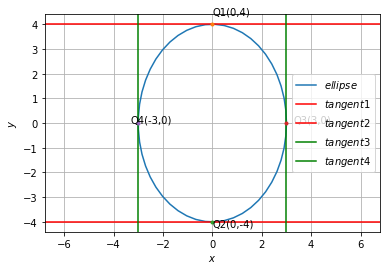
\includegraphics[width=\columnwidth]{./solutions/conics/1/16/ellipse.png}
	\caption{Figure depicting point of contact of tangents of ellipse parallel to x-axis and y-axis}
	\label{eq:solutions/1/16/fig1}
\end{figure}

%
\item Triangles on the same base (or equal bases) and between the same parallels are equal in area.
\\
\solution

General equation of conics is 
\begin{align}
    \vec{x}^T\vec{V}\vec{x}+ 2\vec{u}^T\vec{x}+f = 0
    \label{eq:solutions/1/16/eq:1}
\end{align}
Comparing with the equation given,
\begin{align}
\vec{V}=\myvec{\frac{1}{9} & 0 \\ 0 & \frac{1}{16}}\\
\vec{u}=\vec{0}\\
f=-1\\
\mydet{\vec{v}}=\mydet{\myvec{\frac{1}{9} & 0 \\ 0 & \frac{1}{16}}}>0
\end{align}
$\because \abs{\vec{V}}>0$, the given equation is of ellipse.\\
a)The tangents are parallel to the x-axis, hence, their direction and normal vectors, $\vec{m_1}$ and $\vec{n_1}$ are respectively,
\begin{align}
\vec{m_1}=\myvec{1\\0}\\
\vec{n_1}=\myvec{0\\1}
\end{align}
For an ellipse, given the normal vector $\vec{n}$, the tangent points of contact to the ellipse are given by
\begin{align}
    \vec{q}=\vec{V}^{-1}(\kappa \vec{n}-\vec{u})
    \label{eq:solutions/1/16/eq:2}
    =\vec{V}^{-1}\kappa \vec{n}
\end{align}
where
\begin{align}
    \kappa=\pm \sqrt{\frac{\vec{u^T}\vec{V}^{-1}\vec{u}-f}{\vec{n^T}\vec{V}^{-1}\vec{n}}}
    \label{eq:solutions/1/16/eq:2.0.9}\\
   =\pm \sqrt{\frac{-f}{\vec{n^T}\vec{V}^{-1}\vec{n}}}\\
    \vec{V}^{-1}=\myvec{9 & 0 \\ 0 & 16}\\
    \kappa_1=\pm \sqrt{\frac{-(-1)}{\myvec{0 & 1}\myvec{9 & 0 \\ 0 & 16} \myvec{0\\1}}}\\
 \implies \kappa_1=\pm \sqrt{\frac{1}{16}}\\
    \implies \kappa_1=\pm \frac{1}{4}      
\end{align}
From \eqref{eq:solutions/1/16/eq:2} , the point of contact $\vec{q_i}$ are,
\begin{align}
    \vec{q_1}=\myvec{9 & 0 \\ 0 & 16}\frac{1}{4}\myvec{0\\1}\\
    =\myvec{9 & 0 \\ 0 & 16}\myvec{0\\\frac{1}{4}}\\
    =\myvec{0\\4}\\
    \vec{q_2}=\myvec{9 & 0 \\ 0 & 16}\left(-\frac{1}{4}\right)\ \myvec{0\\1}\\
    =\myvec{9 & 0 \\ 0 & 16}\myvec{0\\-\frac{1}{4}}\\
    =\myvec{0\\-4}
\end{align}
b) The tangents are parallel to the y-axis, hence, their direction and normal vectors, $\vec{m_2}$ and $\vec{n_2}$ are respectively,
\begin{align}
\vec{m_2}=\myvec{0\\1}\\
\vec{n_2}=\myvec{1\\0}
\end{align}
Using equation \eqref{eq:solutions/1/16/eq:2.0.9}, the values of $\kappa$ for this case are
\begin{align}
     \kappa_2=\pm \sqrt{\frac{-(-1)}{\myvec{1 & 0}\myvec{9 & 0 \\ 0 & 16} \myvec{1\\0}}}\\
 \implies \kappa_2=\pm \sqrt{\frac{1}{9}}\\
    \implies \kappa_2=\pm \frac{1}{3} 
\end{align}
and from \eqref{eq:solutions/1/16/eq:2} , the point of contact $\vec{q_i}$ are,
\begin{align}
\vec{q_3}=\myvec{9 & 0 \\ 0 & 16}\frac{1}{3}\myvec{1\\0}\\
    =\myvec{9 & 0 \\ 0 & 16}\myvec{\frac{1}{3}\\0}\\
    =\myvec{3\\0}\\
\vec{q_4}=\myvec{9 & 0 \\ 0 & 16}\left(-\frac{1}{3}\right)\ \myvec{1\\0}\\
    =\myvec{9 & 0 \\ 0 & 16}\myvec{-\frac{1}{3}\\0}\\
    =\myvec{-3\\0}
\end{align}
 \begin{figure}[h!]
	\centering
	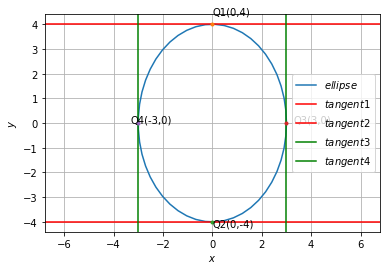
\includegraphics[width=\columnwidth]{./solutions/conics/1/16/ellipse.png}
	\caption{Figure depicting point of contact of tangents of ellipse parallel to x-axis and y-axis}
	\label{eq:solutions/1/16/fig1}
\end{figure}

\item Triangles on the same base (or equal bases) and having equal areas lie between the same parallels.
\\
\solution

General equation of conics is 
\begin{align}
    \vec{x}^T\vec{V}\vec{x}+ 2\vec{u}^T\vec{x}+f = 0
    \label{eq:solutions/1/16/eq:1}
\end{align}
Comparing with the equation given,
\begin{align}
\vec{V}=\myvec{\frac{1}{9} & 0 \\ 0 & \frac{1}{16}}\\
\vec{u}=\vec{0}\\
f=-1\\
\mydet{\vec{v}}=\mydet{\myvec{\frac{1}{9} & 0 \\ 0 & \frac{1}{16}}}>0
\end{align}
$\because \abs{\vec{V}}>0$, the given equation is of ellipse.\\
a)The tangents are parallel to the x-axis, hence, their direction and normal vectors, $\vec{m_1}$ and $\vec{n_1}$ are respectively,
\begin{align}
\vec{m_1}=\myvec{1\\0}\\
\vec{n_1}=\myvec{0\\1}
\end{align}
For an ellipse, given the normal vector $\vec{n}$, the tangent points of contact to the ellipse are given by
\begin{align}
    \vec{q}=\vec{V}^{-1}(\kappa \vec{n}-\vec{u})
    \label{eq:solutions/1/16/eq:2}
    =\vec{V}^{-1}\kappa \vec{n}
\end{align}
where
\begin{align}
    \kappa=\pm \sqrt{\frac{\vec{u^T}\vec{V}^{-1}\vec{u}-f}{\vec{n^T}\vec{V}^{-1}\vec{n}}}
    \label{eq:solutions/1/16/eq:2.0.9}\\
   =\pm \sqrt{\frac{-f}{\vec{n^T}\vec{V}^{-1}\vec{n}}}\\
    \vec{V}^{-1}=\myvec{9 & 0 \\ 0 & 16}\\
    \kappa_1=\pm \sqrt{\frac{-(-1)}{\myvec{0 & 1}\myvec{9 & 0 \\ 0 & 16} \myvec{0\\1}}}\\
 \implies \kappa_1=\pm \sqrt{\frac{1}{16}}\\
    \implies \kappa_1=\pm \frac{1}{4}      
\end{align}
From \eqref{eq:solutions/1/16/eq:2} , the point of contact $\vec{q_i}$ are,
\begin{align}
    \vec{q_1}=\myvec{9 & 0 \\ 0 & 16}\frac{1}{4}\myvec{0\\1}\\
    =\myvec{9 & 0 \\ 0 & 16}\myvec{0\\\frac{1}{4}}\\
    =\myvec{0\\4}\\
    \vec{q_2}=\myvec{9 & 0 \\ 0 & 16}\left(-\frac{1}{4}\right)\ \myvec{0\\1}\\
    =\myvec{9 & 0 \\ 0 & 16}\myvec{0\\-\frac{1}{4}}\\
    =\myvec{0\\-4}
\end{align}
b) The tangents are parallel to the y-axis, hence, their direction and normal vectors, $\vec{m_2}$ and $\vec{n_2}$ are respectively,
\begin{align}
\vec{m_2}=\myvec{0\\1}\\
\vec{n_2}=\myvec{1\\0}
\end{align}
Using equation \eqref{eq:solutions/1/16/eq:2.0.9}, the values of $\kappa$ for this case are
\begin{align}
     \kappa_2=\pm \sqrt{\frac{-(-1)}{\myvec{1 & 0}\myvec{9 & 0 \\ 0 & 16} \myvec{1\\0}}}\\
 \implies \kappa_2=\pm \sqrt{\frac{1}{9}}\\
    \implies \kappa_2=\pm \frac{1}{3} 
\end{align}
and from \eqref{eq:solutions/1/16/eq:2} , the point of contact $\vec{q_i}$ are,
\begin{align}
\vec{q_3}=\myvec{9 & 0 \\ 0 & 16}\frac{1}{3}\myvec{1\\0}\\
    =\myvec{9 & 0 \\ 0 & 16}\myvec{\frac{1}{3}\\0}\\
    =\myvec{3\\0}\\
\vec{q_4}=\myvec{9 & 0 \\ 0 & 16}\left(-\frac{1}{3}\right)\ \myvec{1\\0}\\
    =\myvec{9 & 0 \\ 0 & 16}\myvec{-\frac{1}{3}\\0}\\
    =\myvec{-3\\0}
\end{align}
 \begin{figure}[h!]
	\centering
	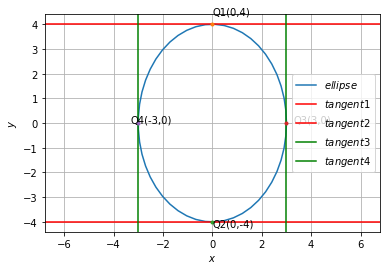
\includegraphics[width=\columnwidth]{./solutions/conics/1/16/ellipse.png}
	\caption{Figure depicting point of contact of tangents of ellipse parallel to x-axis and y-axis}
	\label{eq:solutions/1/16/fig1}
\end{figure}

\item In $\triangle ABC, D, E$ and $F$ are respectively the mid-points of sides $AB, BC$ and $CA $. Show that $\triangle ABC$ is divided into four congruent triangles by joining $D, E$ and $F$.
\\
\solution

General equation of conics is 
\begin{align}
    \vec{x}^T\vec{V}\vec{x}+ 2\vec{u}^T\vec{x}+f = 0
    \label{eq:solutions/1/16/eq:1}
\end{align}
Comparing with the equation given,
\begin{align}
\vec{V}=\myvec{\frac{1}{9} & 0 \\ 0 & \frac{1}{16}}\\
\vec{u}=\vec{0}\\
f=-1\\
\mydet{\vec{v}}=\mydet{\myvec{\frac{1}{9} & 0 \\ 0 & \frac{1}{16}}}>0
\end{align}
$\because \abs{\vec{V}}>0$, the given equation is of ellipse.\\
a)The tangents are parallel to the x-axis, hence, their direction and normal vectors, $\vec{m_1}$ and $\vec{n_1}$ are respectively,
\begin{align}
\vec{m_1}=\myvec{1\\0}\\
\vec{n_1}=\myvec{0\\1}
\end{align}
For an ellipse, given the normal vector $\vec{n}$, the tangent points of contact to the ellipse are given by
\begin{align}
    \vec{q}=\vec{V}^{-1}(\kappa \vec{n}-\vec{u})
    \label{eq:solutions/1/16/eq:2}
    =\vec{V}^{-1}\kappa \vec{n}
\end{align}
where
\begin{align}
    \kappa=\pm \sqrt{\frac{\vec{u^T}\vec{V}^{-1}\vec{u}-f}{\vec{n^T}\vec{V}^{-1}\vec{n}}}
    \label{eq:solutions/1/16/eq:2.0.9}\\
   =\pm \sqrt{\frac{-f}{\vec{n^T}\vec{V}^{-1}\vec{n}}}\\
    \vec{V}^{-1}=\myvec{9 & 0 \\ 0 & 16}\\
    \kappa_1=\pm \sqrt{\frac{-(-1)}{\myvec{0 & 1}\myvec{9 & 0 \\ 0 & 16} \myvec{0\\1}}}\\
 \implies \kappa_1=\pm \sqrt{\frac{1}{16}}\\
    \implies \kappa_1=\pm \frac{1}{4}      
\end{align}
From \eqref{eq:solutions/1/16/eq:2} , the point of contact $\vec{q_i}$ are,
\begin{align}
    \vec{q_1}=\myvec{9 & 0 \\ 0 & 16}\frac{1}{4}\myvec{0\\1}\\
    =\myvec{9 & 0 \\ 0 & 16}\myvec{0\\\frac{1}{4}}\\
    =\myvec{0\\4}\\
    \vec{q_2}=\myvec{9 & 0 \\ 0 & 16}\left(-\frac{1}{4}\right)\ \myvec{0\\1}\\
    =\myvec{9 & 0 \\ 0 & 16}\myvec{0\\-\frac{1}{4}}\\
    =\myvec{0\\-4}
\end{align}
b) The tangents are parallel to the y-axis, hence, their direction and normal vectors, $\vec{m_2}$ and $\vec{n_2}$ are respectively,
\begin{align}
\vec{m_2}=\myvec{0\\1}\\
\vec{n_2}=\myvec{1\\0}
\end{align}
Using equation \eqref{eq:solutions/1/16/eq:2.0.9}, the values of $\kappa$ for this case are
\begin{align}
     \kappa_2=\pm \sqrt{\frac{-(-1)}{\myvec{1 & 0}\myvec{9 & 0 \\ 0 & 16} \myvec{1\\0}}}\\
 \implies \kappa_2=\pm \sqrt{\frac{1}{9}}\\
    \implies \kappa_2=\pm \frac{1}{3} 
\end{align}
and from \eqref{eq:solutions/1/16/eq:2} , the point of contact $\vec{q_i}$ are,
\begin{align}
\vec{q_3}=\myvec{9 & 0 \\ 0 & 16}\frac{1}{3}\myvec{1\\0}\\
    =\myvec{9 & 0 \\ 0 & 16}\myvec{\frac{1}{3}\\0}\\
    =\myvec{3\\0}\\
\vec{q_4}=\myvec{9 & 0 \\ 0 & 16}\left(-\frac{1}{3}\right)\ \myvec{1\\0}\\
    =\myvec{9 & 0 \\ 0 & 16}\myvec{-\frac{1}{3}\\0}\\
    =\myvec{-3\\0}
\end{align}
 \begin{figure}[h!]
	\centering
	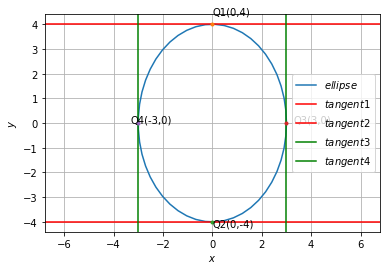
\includegraphics[width=\columnwidth]{./solutions/conics/1/16/ellipse.png}
	\caption{Figure depicting point of contact of tangents of ellipse parallel to x-axis and y-axis}
	\label{eq:solutions/1/16/fig1}
\end{figure}

\item  The line-segment joining the mid-points of any two sides of a triangle is parallel to the third side and is half of it.
\label{prob:tri_mid_similar}
\\
\solution

General equation of conics is 
\begin{align}
    \vec{x}^T\vec{V}\vec{x}+ 2\vec{u}^T\vec{x}+f = 0
    \label{eq:solutions/1/16/eq:1}
\end{align}
Comparing with the equation given,
\begin{align}
\vec{V}=\myvec{\frac{1}{9} & 0 \\ 0 & \frac{1}{16}}\\
\vec{u}=\vec{0}\\
f=-1\\
\mydet{\vec{v}}=\mydet{\myvec{\frac{1}{9} & 0 \\ 0 & \frac{1}{16}}}>0
\end{align}
$\because \abs{\vec{V}}>0$, the given equation is of ellipse.\\
a)The tangents are parallel to the x-axis, hence, their direction and normal vectors, $\vec{m_1}$ and $\vec{n_1}$ are respectively,
\begin{align}
\vec{m_1}=\myvec{1\\0}\\
\vec{n_1}=\myvec{0\\1}
\end{align}
For an ellipse, given the normal vector $\vec{n}$, the tangent points of contact to the ellipse are given by
\begin{align}
    \vec{q}=\vec{V}^{-1}(\kappa \vec{n}-\vec{u})
    \label{eq:solutions/1/16/eq:2}
    =\vec{V}^{-1}\kappa \vec{n}
\end{align}
where
\begin{align}
    \kappa=\pm \sqrt{\frac{\vec{u^T}\vec{V}^{-1}\vec{u}-f}{\vec{n^T}\vec{V}^{-1}\vec{n}}}
    \label{eq:solutions/1/16/eq:2.0.9}\\
   =\pm \sqrt{\frac{-f}{\vec{n^T}\vec{V}^{-1}\vec{n}}}\\
    \vec{V}^{-1}=\myvec{9 & 0 \\ 0 & 16}\\
    \kappa_1=\pm \sqrt{\frac{-(-1)}{\myvec{0 & 1}\myvec{9 & 0 \\ 0 & 16} \myvec{0\\1}}}\\
 \implies \kappa_1=\pm \sqrt{\frac{1}{16}}\\
    \implies \kappa_1=\pm \frac{1}{4}      
\end{align}
From \eqref{eq:solutions/1/16/eq:2} , the point of contact $\vec{q_i}$ are,
\begin{align}
    \vec{q_1}=\myvec{9 & 0 \\ 0 & 16}\frac{1}{4}\myvec{0\\1}\\
    =\myvec{9 & 0 \\ 0 & 16}\myvec{0\\\frac{1}{4}}\\
    =\myvec{0\\4}\\
    \vec{q_2}=\myvec{9 & 0 \\ 0 & 16}\left(-\frac{1}{4}\right)\ \myvec{0\\1}\\
    =\myvec{9 & 0 \\ 0 & 16}\myvec{0\\-\frac{1}{4}}\\
    =\myvec{0\\-4}
\end{align}
b) The tangents are parallel to the y-axis, hence, their direction and normal vectors, $\vec{m_2}$ and $\vec{n_2}$ are respectively,
\begin{align}
\vec{m_2}=\myvec{0\\1}\\
\vec{n_2}=\myvec{1\\0}
\end{align}
Using equation \eqref{eq:solutions/1/16/eq:2.0.9}, the values of $\kappa$ for this case are
\begin{align}
     \kappa_2=\pm \sqrt{\frac{-(-1)}{\myvec{1 & 0}\myvec{9 & 0 \\ 0 & 16} \myvec{1\\0}}}\\
 \implies \kappa_2=\pm \sqrt{\frac{1}{9}}\\
    \implies \kappa_2=\pm \frac{1}{3} 
\end{align}
and from \eqref{eq:solutions/1/16/eq:2} , the point of contact $\vec{q_i}$ are,
\begin{align}
\vec{q_3}=\myvec{9 & 0 \\ 0 & 16}\frac{1}{3}\myvec{1\\0}\\
    =\myvec{9 & 0 \\ 0 & 16}\myvec{\frac{1}{3}\\0}\\
    =\myvec{3\\0}\\
\vec{q_4}=\myvec{9 & 0 \\ 0 & 16}\left(-\frac{1}{3}\right)\ \myvec{1\\0}\\
    =\myvec{9 & 0 \\ 0 & 16}\myvec{-\frac{1}{3}\\0}\\
    =\myvec{-3\\0}
\end{align}
 \begin{figure}[h!]
	\centering
	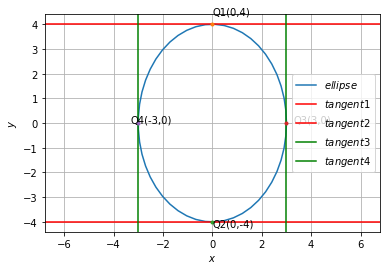
\includegraphics[width=\columnwidth]{./solutions/conics/1/16/ellipse.png}
	\caption{Figure depicting point of contact of tangents of ellipse parallel to x-axis and y-axis}
	\label{eq:solutions/1/16/fig1}
\end{figure}

%\label{prob:quad_similar}
%%
%\\
%\solution If $DE$ is the lie joining he mid points of $\triangle ABC$,  use cosine formula to find the lengths of $DE$ and $BC$. Then use cosine formula to show that all angles of $\triangle ADE$ are equal to the corresponding angles of $\triangle ABC$.
%
\item  A line through the mid-point of a side of a triangle parallel to another side 
bisects the third side.
\\
\solution

General equation of conics is 
\begin{align}
    \vec{x}^T\vec{V}\vec{x}+ 2\vec{u}^T\vec{x}+f = 0
    \label{eq:solutions/1/16/eq:1}
\end{align}
Comparing with the equation given,
\begin{align}
\vec{V}=\myvec{\frac{1}{9} & 0 \\ 0 & \frac{1}{16}}\\
\vec{u}=\vec{0}\\
f=-1\\
\mydet{\vec{v}}=\mydet{\myvec{\frac{1}{9} & 0 \\ 0 & \frac{1}{16}}}>0
\end{align}
$\because \abs{\vec{V}}>0$, the given equation is of ellipse.\\
a)The tangents are parallel to the x-axis, hence, their direction and normal vectors, $\vec{m_1}$ and $\vec{n_1}$ are respectively,
\begin{align}
\vec{m_1}=\myvec{1\\0}\\
\vec{n_1}=\myvec{0\\1}
\end{align}
For an ellipse, given the normal vector $\vec{n}$, the tangent points of contact to the ellipse are given by
\begin{align}
    \vec{q}=\vec{V}^{-1}(\kappa \vec{n}-\vec{u})
    \label{eq:solutions/1/16/eq:2}
    =\vec{V}^{-1}\kappa \vec{n}
\end{align}
where
\begin{align}
    \kappa=\pm \sqrt{\frac{\vec{u^T}\vec{V}^{-1}\vec{u}-f}{\vec{n^T}\vec{V}^{-1}\vec{n}}}
    \label{eq:solutions/1/16/eq:2.0.9}\\
   =\pm \sqrt{\frac{-f}{\vec{n^T}\vec{V}^{-1}\vec{n}}}\\
    \vec{V}^{-1}=\myvec{9 & 0 \\ 0 & 16}\\
    \kappa_1=\pm \sqrt{\frac{-(-1)}{\myvec{0 & 1}\myvec{9 & 0 \\ 0 & 16} \myvec{0\\1}}}\\
 \implies \kappa_1=\pm \sqrt{\frac{1}{16}}\\
    \implies \kappa_1=\pm \frac{1}{4}      
\end{align}
From \eqref{eq:solutions/1/16/eq:2} , the point of contact $\vec{q_i}$ are,
\begin{align}
    \vec{q_1}=\myvec{9 & 0 \\ 0 & 16}\frac{1}{4}\myvec{0\\1}\\
    =\myvec{9 & 0 \\ 0 & 16}\myvec{0\\\frac{1}{4}}\\
    =\myvec{0\\4}\\
    \vec{q_2}=\myvec{9 & 0 \\ 0 & 16}\left(-\frac{1}{4}\right)\ \myvec{0\\1}\\
    =\myvec{9 & 0 \\ 0 & 16}\myvec{0\\-\frac{1}{4}}\\
    =\myvec{0\\-4}
\end{align}
b) The tangents are parallel to the y-axis, hence, their direction and normal vectors, $\vec{m_2}$ and $\vec{n_2}$ are respectively,
\begin{align}
\vec{m_2}=\myvec{0\\1}\\
\vec{n_2}=\myvec{1\\0}
\end{align}
Using equation \eqref{eq:solutions/1/16/eq:2.0.9}, the values of $\kappa$ for this case are
\begin{align}
     \kappa_2=\pm \sqrt{\frac{-(-1)}{\myvec{1 & 0}\myvec{9 & 0 \\ 0 & 16} \myvec{1\\0}}}\\
 \implies \kappa_2=\pm \sqrt{\frac{1}{9}}\\
    \implies \kappa_2=\pm \frac{1}{3} 
\end{align}
and from \eqref{eq:solutions/1/16/eq:2} , the point of contact $\vec{q_i}$ are,
\begin{align}
\vec{q_3}=\myvec{9 & 0 \\ 0 & 16}\frac{1}{3}\myvec{1\\0}\\
    =\myvec{9 & 0 \\ 0 & 16}\myvec{\frac{1}{3}\\0}\\
    =\myvec{3\\0}\\
\vec{q_4}=\myvec{9 & 0 \\ 0 & 16}\left(-\frac{1}{3}\right)\ \myvec{1\\0}\\
    =\myvec{9 & 0 \\ 0 & 16}\myvec{-\frac{1}{3}\\0}\\
    =\myvec{-3\\0}
\end{align}
 \begin{figure}[h!]
	\centering
	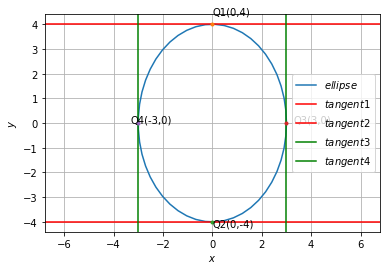
\includegraphics[width=\columnwidth]{./solutions/conics/1/16/ellipse.png}
	\caption{Figure depicting point of contact of tangents of ellipse parallel to x-axis and y-axis}
	\label{eq:solutions/1/16/fig1}
\end{figure}

%\\
%\solution Use cosine formula.

\item ABC is a triangle right angled at $C$. A line through the mid-point $M$ of hypotenuse $AB$ and parallel to $BC$ intersects $AC$ at $D$. Show that (i) $D$ is the mid-point of $AC$
(ii) $MD \perp AC$ (iii) $CM = MA = \frac{1}{2}AB$
\\
\solution

General equation of conics is 
\begin{align}
    \vec{x}^T\vec{V}\vec{x}+ 2\vec{u}^T\vec{x}+f = 0
    \label{eq:solutions/1/16/eq:1}
\end{align}
Comparing with the equation given,
\begin{align}
\vec{V}=\myvec{\frac{1}{9} & 0 \\ 0 & \frac{1}{16}}\\
\vec{u}=\vec{0}\\
f=-1\\
\mydet{\vec{v}}=\mydet{\myvec{\frac{1}{9} & 0 \\ 0 & \frac{1}{16}}}>0
\end{align}
$\because \abs{\vec{V}}>0$, the given equation is of ellipse.\\
a)The tangents are parallel to the x-axis, hence, their direction and normal vectors, $\vec{m_1}$ and $\vec{n_1}$ are respectively,
\begin{align}
\vec{m_1}=\myvec{1\\0}\\
\vec{n_1}=\myvec{0\\1}
\end{align}
For an ellipse, given the normal vector $\vec{n}$, the tangent points of contact to the ellipse are given by
\begin{align}
    \vec{q}=\vec{V}^{-1}(\kappa \vec{n}-\vec{u})
    \label{eq:solutions/1/16/eq:2}
    =\vec{V}^{-1}\kappa \vec{n}
\end{align}
where
\begin{align}
    \kappa=\pm \sqrt{\frac{\vec{u^T}\vec{V}^{-1}\vec{u}-f}{\vec{n^T}\vec{V}^{-1}\vec{n}}}
    \label{eq:solutions/1/16/eq:2.0.9}\\
   =\pm \sqrt{\frac{-f}{\vec{n^T}\vec{V}^{-1}\vec{n}}}\\
    \vec{V}^{-1}=\myvec{9 & 0 \\ 0 & 16}\\
    \kappa_1=\pm \sqrt{\frac{-(-1)}{\myvec{0 & 1}\myvec{9 & 0 \\ 0 & 16} \myvec{0\\1}}}\\
 \implies \kappa_1=\pm \sqrt{\frac{1}{16}}\\
    \implies \kappa_1=\pm \frac{1}{4}      
\end{align}
From \eqref{eq:solutions/1/16/eq:2} , the point of contact $\vec{q_i}$ are,
\begin{align}
    \vec{q_1}=\myvec{9 & 0 \\ 0 & 16}\frac{1}{4}\myvec{0\\1}\\
    =\myvec{9 & 0 \\ 0 & 16}\myvec{0\\\frac{1}{4}}\\
    =\myvec{0\\4}\\
    \vec{q_2}=\myvec{9 & 0 \\ 0 & 16}\left(-\frac{1}{4}\right)\ \myvec{0\\1}\\
    =\myvec{9 & 0 \\ 0 & 16}\myvec{0\\-\frac{1}{4}}\\
    =\myvec{0\\-4}
\end{align}
b) The tangents are parallel to the y-axis, hence, their direction and normal vectors, $\vec{m_2}$ and $\vec{n_2}$ are respectively,
\begin{align}
\vec{m_2}=\myvec{0\\1}\\
\vec{n_2}=\myvec{1\\0}
\end{align}
Using equation \eqref{eq:solutions/1/16/eq:2.0.9}, the values of $\kappa$ for this case are
\begin{align}
     \kappa_2=\pm \sqrt{\frac{-(-1)}{\myvec{1 & 0}\myvec{9 & 0 \\ 0 & 16} \myvec{1\\0}}}\\
 \implies \kappa_2=\pm \sqrt{\frac{1}{9}}\\
    \implies \kappa_2=\pm \frac{1}{3} 
\end{align}
and from \eqref{eq:solutions/1/16/eq:2} , the point of contact $\vec{q_i}$ are,
\begin{align}
\vec{q_3}=\myvec{9 & 0 \\ 0 & 16}\frac{1}{3}\myvec{1\\0}\\
    =\myvec{9 & 0 \\ 0 & 16}\myvec{\frac{1}{3}\\0}\\
    =\myvec{3\\0}\\
\vec{q_4}=\myvec{9 & 0 \\ 0 & 16}\left(-\frac{1}{3}\right)\ \myvec{1\\0}\\
    =\myvec{9 & 0 \\ 0 & 16}\myvec{-\frac{1}{3}\\0}\\
    =\myvec{-3\\0}
\end{align}
 \begin{figure}[h!]
	\centering
	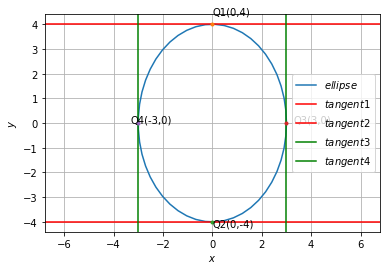
\includegraphics[width=\columnwidth]{./solutions/conics/1/16/ellipse.png}
	\caption{Figure depicting point of contact of tangents of ellipse parallel to x-axis and y-axis}
	\label{eq:solutions/1/16/fig1}
\end{figure}


\item  Sides opposite to equal angles of a triangle are equal. 
\\
\solution

General equation of conics is 
\begin{align}
    \vec{x}^T\vec{V}\vec{x}+ 2\vec{u}^T\vec{x}+f = 0
    \label{eq:solutions/1/16/eq:1}
\end{align}
Comparing with the equation given,
\begin{align}
\vec{V}=\myvec{\frac{1}{9} & 0 \\ 0 & \frac{1}{16}}\\
\vec{u}=\vec{0}\\
f=-1\\
\mydet{\vec{v}}=\mydet{\myvec{\frac{1}{9} & 0 \\ 0 & \frac{1}{16}}}>0
\end{align}
$\because \abs{\vec{V}}>0$, the given equation is of ellipse.\\
a)The tangents are parallel to the x-axis, hence, their direction and normal vectors, $\vec{m_1}$ and $\vec{n_1}$ are respectively,
\begin{align}
\vec{m_1}=\myvec{1\\0}\\
\vec{n_1}=\myvec{0\\1}
\end{align}
For an ellipse, given the normal vector $\vec{n}$, the tangent points of contact to the ellipse are given by
\begin{align}
    \vec{q}=\vec{V}^{-1}(\kappa \vec{n}-\vec{u})
    \label{eq:solutions/1/16/eq:2}
    =\vec{V}^{-1}\kappa \vec{n}
\end{align}
where
\begin{align}
    \kappa=\pm \sqrt{\frac{\vec{u^T}\vec{V}^{-1}\vec{u}-f}{\vec{n^T}\vec{V}^{-1}\vec{n}}}
    \label{eq:solutions/1/16/eq:2.0.9}\\
   =\pm \sqrt{\frac{-f}{\vec{n^T}\vec{V}^{-1}\vec{n}}}\\
    \vec{V}^{-1}=\myvec{9 & 0 \\ 0 & 16}\\
    \kappa_1=\pm \sqrt{\frac{-(-1)}{\myvec{0 & 1}\myvec{9 & 0 \\ 0 & 16} \myvec{0\\1}}}\\
 \implies \kappa_1=\pm \sqrt{\frac{1}{16}}\\
    \implies \kappa_1=\pm \frac{1}{4}      
\end{align}
From \eqref{eq:solutions/1/16/eq:2} , the point of contact $\vec{q_i}$ are,
\begin{align}
    \vec{q_1}=\myvec{9 & 0 \\ 0 & 16}\frac{1}{4}\myvec{0\\1}\\
    =\myvec{9 & 0 \\ 0 & 16}\myvec{0\\\frac{1}{4}}\\
    =\myvec{0\\4}\\
    \vec{q_2}=\myvec{9 & 0 \\ 0 & 16}\left(-\frac{1}{4}\right)\ \myvec{0\\1}\\
    =\myvec{9 & 0 \\ 0 & 16}\myvec{0\\-\frac{1}{4}}\\
    =\myvec{0\\-4}
\end{align}
b) The tangents are parallel to the y-axis, hence, their direction and normal vectors, $\vec{m_2}$ and $\vec{n_2}$ are respectively,
\begin{align}
\vec{m_2}=\myvec{0\\1}\\
\vec{n_2}=\myvec{1\\0}
\end{align}
Using equation \eqref{eq:solutions/1/16/eq:2.0.9}, the values of $\kappa$ for this case are
\begin{align}
     \kappa_2=\pm \sqrt{\frac{-(-1)}{\myvec{1 & 0}\myvec{9 & 0 \\ 0 & 16} \myvec{1\\0}}}\\
 \implies \kappa_2=\pm \sqrt{\frac{1}{9}}\\
    \implies \kappa_2=\pm \frac{1}{3} 
\end{align}
and from \eqref{eq:solutions/1/16/eq:2} , the point of contact $\vec{q_i}$ are,
\begin{align}
\vec{q_3}=\myvec{9 & 0 \\ 0 & 16}\frac{1}{3}\myvec{1\\0}\\
    =\myvec{9 & 0 \\ 0 & 16}\myvec{\frac{1}{3}\\0}\\
    =\myvec{3\\0}\\
\vec{q_4}=\myvec{9 & 0 \\ 0 & 16}\left(-\frac{1}{3}\right)\ \myvec{1\\0}\\
    =\myvec{9 & 0 \\ 0 & 16}\myvec{-\frac{1}{3}\\0}\\
    =\myvec{-3\\0}
\end{align}
 \begin{figure}[h!]
	\centering
	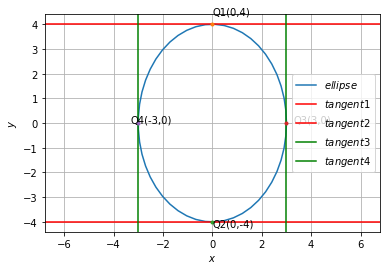
\includegraphics[width=\columnwidth]{./solutions/conics/1/16/ellipse.png}
	\caption{Figure depicting point of contact of tangents of ellipse parallel to x-axis and y-axis}
	\label{eq:solutions/1/16/fig1}
\end{figure}

%\\
%\solution Use \eqref{eq:tri_sin_form} and the argument in Problem \ref{prob:tri_ang_side_eq}
%
\item $AB$ is a line-segment. $P$ and $Q$ are points on opposite sides of $AB$ such that each of them is equidistant from the points $A$ and $B$. Show that the line $PQ $ is the perpendicular bisector of $AB$.
\\
\solution

General equation of conics is 
\begin{align}
    \vec{x}^T\vec{V}\vec{x}+ 2\vec{u}^T\vec{x}+f = 0
    \label{eq:solutions/1/16/eq:1}
\end{align}
Comparing with the equation given,
\begin{align}
\vec{V}=\myvec{\frac{1}{9} & 0 \\ 0 & \frac{1}{16}}\\
\vec{u}=\vec{0}\\
f=-1\\
\mydet{\vec{v}}=\mydet{\myvec{\frac{1}{9} & 0 \\ 0 & \frac{1}{16}}}>0
\end{align}
$\because \abs{\vec{V}}>0$, the given equation is of ellipse.\\
a)The tangents are parallel to the x-axis, hence, their direction and normal vectors, $\vec{m_1}$ and $\vec{n_1}$ are respectively,
\begin{align}
\vec{m_1}=\myvec{1\\0}\\
\vec{n_1}=\myvec{0\\1}
\end{align}
For an ellipse, given the normal vector $\vec{n}$, the tangent points of contact to the ellipse are given by
\begin{align}
    \vec{q}=\vec{V}^{-1}(\kappa \vec{n}-\vec{u})
    \label{eq:solutions/1/16/eq:2}
    =\vec{V}^{-1}\kappa \vec{n}
\end{align}
where
\begin{align}
    \kappa=\pm \sqrt{\frac{\vec{u^T}\vec{V}^{-1}\vec{u}-f}{\vec{n^T}\vec{V}^{-1}\vec{n}}}
    \label{eq:solutions/1/16/eq:2.0.9}\\
   =\pm \sqrt{\frac{-f}{\vec{n^T}\vec{V}^{-1}\vec{n}}}\\
    \vec{V}^{-1}=\myvec{9 & 0 \\ 0 & 16}\\
    \kappa_1=\pm \sqrt{\frac{-(-1)}{\myvec{0 & 1}\myvec{9 & 0 \\ 0 & 16} \myvec{0\\1}}}\\
 \implies \kappa_1=\pm \sqrt{\frac{1}{16}}\\
    \implies \kappa_1=\pm \frac{1}{4}      
\end{align}
From \eqref{eq:solutions/1/16/eq:2} , the point of contact $\vec{q_i}$ are,
\begin{align}
    \vec{q_1}=\myvec{9 & 0 \\ 0 & 16}\frac{1}{4}\myvec{0\\1}\\
    =\myvec{9 & 0 \\ 0 & 16}\myvec{0\\\frac{1}{4}}\\
    =\myvec{0\\4}\\
    \vec{q_2}=\myvec{9 & 0 \\ 0 & 16}\left(-\frac{1}{4}\right)\ \myvec{0\\1}\\
    =\myvec{9 & 0 \\ 0 & 16}\myvec{0\\-\frac{1}{4}}\\
    =\myvec{0\\-4}
\end{align}
b) The tangents are parallel to the y-axis, hence, their direction and normal vectors, $\vec{m_2}$ and $\vec{n_2}$ are respectively,
\begin{align}
\vec{m_2}=\myvec{0\\1}\\
\vec{n_2}=\myvec{1\\0}
\end{align}
Using equation \eqref{eq:solutions/1/16/eq:2.0.9}, the values of $\kappa$ for this case are
\begin{align}
     \kappa_2=\pm \sqrt{\frac{-(-1)}{\myvec{1 & 0}\myvec{9 & 0 \\ 0 & 16} \myvec{1\\0}}}\\
 \implies \kappa_2=\pm \sqrt{\frac{1}{9}}\\
    \implies \kappa_2=\pm \frac{1}{3} 
\end{align}
and from \eqref{eq:solutions/1/16/eq:2} , the point of contact $\vec{q_i}$ are,
\begin{align}
\vec{q_3}=\myvec{9 & 0 \\ 0 & 16}\frac{1}{3}\myvec{1\\0}\\
    =\myvec{9 & 0 \\ 0 & 16}\myvec{\frac{1}{3}\\0}\\
    =\myvec{3\\0}\\
\vec{q_4}=\myvec{9 & 0 \\ 0 & 16}\left(-\frac{1}{3}\right)\ \myvec{1\\0}\\
    =\myvec{9 & 0 \\ 0 & 16}\myvec{-\frac{1}{3}\\0}\\
    =\myvec{-3\\0}
\end{align}
 \begin{figure}[h!]
	\centering
	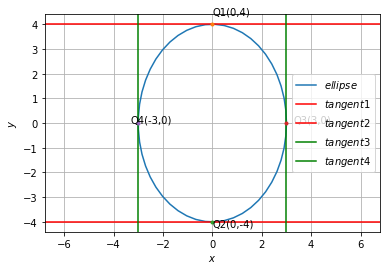
\includegraphics[width=\columnwidth]{./solutions/conics/1/16/ellipse.png}
	\caption{Figure depicting point of contact of tangents of ellipse parallel to x-axis and y-axis}
	\label{eq:solutions/1/16/fig1}
\end{figure}

%\\
%\solution In an equilateral $\triangle$, 
%%
%\begin{align}
%A=B=C.&
%\\
%\because A+B+C = 180\degree, 3A = 180\degree&
%\\
%\implies A = 60\degree&
%\end{align}
%
\item Show that $\cos 60\degree = \frac{1}{2} $.  
\\
\solution

General equation of conics is 
\begin{align}
    \vec{x}^T\vec{V}\vec{x}+ 2\vec{u}^T\vec{x}+f = 0
    \label{eq:solutions/1/16/eq:1}
\end{align}
Comparing with the equation given,
\begin{align}
\vec{V}=\myvec{\frac{1}{9} & 0 \\ 0 & \frac{1}{16}}\\
\vec{u}=\vec{0}\\
f=-1\\
\mydet{\vec{v}}=\mydet{\myvec{\frac{1}{9} & 0 \\ 0 & \frac{1}{16}}}>0
\end{align}
$\because \abs{\vec{V}}>0$, the given equation is of ellipse.\\
a)The tangents are parallel to the x-axis, hence, their direction and normal vectors, $\vec{m_1}$ and $\vec{n_1}$ are respectively,
\begin{align}
\vec{m_1}=\myvec{1\\0}\\
\vec{n_1}=\myvec{0\\1}
\end{align}
For an ellipse, given the normal vector $\vec{n}$, the tangent points of contact to the ellipse are given by
\begin{align}
    \vec{q}=\vec{V}^{-1}(\kappa \vec{n}-\vec{u})
    \label{eq:solutions/1/16/eq:2}
    =\vec{V}^{-1}\kappa \vec{n}
\end{align}
where
\begin{align}
    \kappa=\pm \sqrt{\frac{\vec{u^T}\vec{V}^{-1}\vec{u}-f}{\vec{n^T}\vec{V}^{-1}\vec{n}}}
    \label{eq:solutions/1/16/eq:2.0.9}\\
   =\pm \sqrt{\frac{-f}{\vec{n^T}\vec{V}^{-1}\vec{n}}}\\
    \vec{V}^{-1}=\myvec{9 & 0 \\ 0 & 16}\\
    \kappa_1=\pm \sqrt{\frac{-(-1)}{\myvec{0 & 1}\myvec{9 & 0 \\ 0 & 16} \myvec{0\\1}}}\\
 \implies \kappa_1=\pm \sqrt{\frac{1}{16}}\\
    \implies \kappa_1=\pm \frac{1}{4}      
\end{align}
From \eqref{eq:solutions/1/16/eq:2} , the point of contact $\vec{q_i}$ are,
\begin{align}
    \vec{q_1}=\myvec{9 & 0 \\ 0 & 16}\frac{1}{4}\myvec{0\\1}\\
    =\myvec{9 & 0 \\ 0 & 16}\myvec{0\\\frac{1}{4}}\\
    =\myvec{0\\4}\\
    \vec{q_2}=\myvec{9 & 0 \\ 0 & 16}\left(-\frac{1}{4}\right)\ \myvec{0\\1}\\
    =\myvec{9 & 0 \\ 0 & 16}\myvec{0\\-\frac{1}{4}}\\
    =\myvec{0\\-4}
\end{align}
b) The tangents are parallel to the y-axis, hence, their direction and normal vectors, $\vec{m_2}$ and $\vec{n_2}$ are respectively,
\begin{align}
\vec{m_2}=\myvec{0\\1}\\
\vec{n_2}=\myvec{1\\0}
\end{align}
Using equation \eqref{eq:solutions/1/16/eq:2.0.9}, the values of $\kappa$ for this case are
\begin{align}
     \kappa_2=\pm \sqrt{\frac{-(-1)}{\myvec{1 & 0}\myvec{9 & 0 \\ 0 & 16} \myvec{1\\0}}}\\
 \implies \kappa_2=\pm \sqrt{\frac{1}{9}}\\
    \implies \kappa_2=\pm \frac{1}{3} 
\end{align}
and from \eqref{eq:solutions/1/16/eq:2} , the point of contact $\vec{q_i}$ are,
\begin{align}
\vec{q_3}=\myvec{9 & 0 \\ 0 & 16}\frac{1}{3}\myvec{1\\0}\\
    =\myvec{9 & 0 \\ 0 & 16}\myvec{\frac{1}{3}\\0}\\
    =\myvec{3\\0}\\
\vec{q_4}=\myvec{9 & 0 \\ 0 & 16}\left(-\frac{1}{3}\right)\ \myvec{1\\0}\\
    =\myvec{9 & 0 \\ 0 & 16}\myvec{-\frac{1}{3}\\0}\\
    =\myvec{-3\\0}
\end{align}
 \begin{figure}[h!]
	\centering
	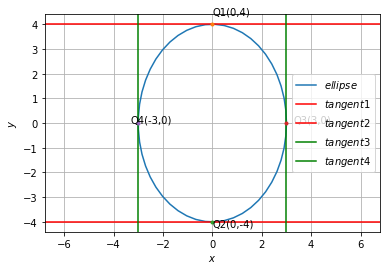
\includegraphics[width=\columnwidth]{./solutions/conics/1/16/ellipse.png}
	\caption{Figure depicting point of contact of tangents of ellipse parallel to x-axis and y-axis}
	\label{eq:solutions/1/16/fig1}
\end{figure}

\item Show that $\sin 60\degree = \frac{\sqrt{3}}{2} $.
\\
\solution

General equation of conics is 
\begin{align}
    \vec{x}^T\vec{V}\vec{x}+ 2\vec{u}^T\vec{x}+f = 0
    \label{eq:solutions/1/16/eq:1}
\end{align}
Comparing with the equation given,
\begin{align}
\vec{V}=\myvec{\frac{1}{9} & 0 \\ 0 & \frac{1}{16}}\\
\vec{u}=\vec{0}\\
f=-1\\
\mydet{\vec{v}}=\mydet{\myvec{\frac{1}{9} & 0 \\ 0 & \frac{1}{16}}}>0
\end{align}
$\because \abs{\vec{V}}>0$, the given equation is of ellipse.\\
a)The tangents are parallel to the x-axis, hence, their direction and normal vectors, $\vec{m_1}$ and $\vec{n_1}$ are respectively,
\begin{align}
\vec{m_1}=\myvec{1\\0}\\
\vec{n_1}=\myvec{0\\1}
\end{align}
For an ellipse, given the normal vector $\vec{n}$, the tangent points of contact to the ellipse are given by
\begin{align}
    \vec{q}=\vec{V}^{-1}(\kappa \vec{n}-\vec{u})
    \label{eq:solutions/1/16/eq:2}
    =\vec{V}^{-1}\kappa \vec{n}
\end{align}
where
\begin{align}
    \kappa=\pm \sqrt{\frac{\vec{u^T}\vec{V}^{-1}\vec{u}-f}{\vec{n^T}\vec{V}^{-1}\vec{n}}}
    \label{eq:solutions/1/16/eq:2.0.9}\\
   =\pm \sqrt{\frac{-f}{\vec{n^T}\vec{V}^{-1}\vec{n}}}\\
    \vec{V}^{-1}=\myvec{9 & 0 \\ 0 & 16}\\
    \kappa_1=\pm \sqrt{\frac{-(-1)}{\myvec{0 & 1}\myvec{9 & 0 \\ 0 & 16} \myvec{0\\1}}}\\
 \implies \kappa_1=\pm \sqrt{\frac{1}{16}}\\
    \implies \kappa_1=\pm \frac{1}{4}      
\end{align}
From \eqref{eq:solutions/1/16/eq:2} , the point of contact $\vec{q_i}$ are,
\begin{align}
    \vec{q_1}=\myvec{9 & 0 \\ 0 & 16}\frac{1}{4}\myvec{0\\1}\\
    =\myvec{9 & 0 \\ 0 & 16}\myvec{0\\\frac{1}{4}}\\
    =\myvec{0\\4}\\
    \vec{q_2}=\myvec{9 & 0 \\ 0 & 16}\left(-\frac{1}{4}\right)\ \myvec{0\\1}\\
    =\myvec{9 & 0 \\ 0 & 16}\myvec{0\\-\frac{1}{4}}\\
    =\myvec{0\\-4}
\end{align}
b) The tangents are parallel to the y-axis, hence, their direction and normal vectors, $\vec{m_2}$ and $\vec{n_2}$ are respectively,
\begin{align}
\vec{m_2}=\myvec{0\\1}\\
\vec{n_2}=\myvec{1\\0}
\end{align}
Using equation \eqref{eq:solutions/1/16/eq:2.0.9}, the values of $\kappa$ for this case are
\begin{align}
     \kappa_2=\pm \sqrt{\frac{-(-1)}{\myvec{1 & 0}\myvec{9 & 0 \\ 0 & 16} \myvec{1\\0}}}\\
 \implies \kappa_2=\pm \sqrt{\frac{1}{9}}\\
    \implies \kappa_2=\pm \frac{1}{3} 
\end{align}
and from \eqref{eq:solutions/1/16/eq:2} , the point of contact $\vec{q_i}$ are,
\begin{align}
\vec{q_3}=\myvec{9 & 0 \\ 0 & 16}\frac{1}{3}\myvec{1\\0}\\
    =\myvec{9 & 0 \\ 0 & 16}\myvec{\frac{1}{3}\\0}\\
    =\myvec{3\\0}\\
\vec{q_4}=\myvec{9 & 0 \\ 0 & 16}\left(-\frac{1}{3}\right)\ \myvec{1\\0}\\
    =\myvec{9 & 0 \\ 0 & 16}\myvec{-\frac{1}{3}\\0}\\
    =\myvec{-3\\0}
\end{align}
 \begin{figure}[h!]
	\centering
	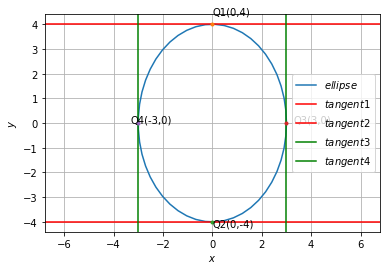
\includegraphics[width=\columnwidth]{./solutions/conics/1/16/ellipse.png}
	\caption{Figure depicting point of contact of tangents of ellipse parallel to x-axis and y-axis}
	\label{eq:solutions/1/16/fig1}
\end{figure}

\item Find  $\sin 30\degree$ and  $\cos 30\degree$.
\\
\solution

General equation of conics is 
\begin{align}
    \vec{x}^T\vec{V}\vec{x}+ 2\vec{u}^T\vec{x}+f = 0
    \label{eq:solutions/1/16/eq:1}
\end{align}
Comparing with the equation given,
\begin{align}
\vec{V}=\myvec{\frac{1}{9} & 0 \\ 0 & \frac{1}{16}}\\
\vec{u}=\vec{0}\\
f=-1\\
\mydet{\vec{v}}=\mydet{\myvec{\frac{1}{9} & 0 \\ 0 & \frac{1}{16}}}>0
\end{align}
$\because \abs{\vec{V}}>0$, the given equation is of ellipse.\\
a)The tangents are parallel to the x-axis, hence, their direction and normal vectors, $\vec{m_1}$ and $\vec{n_1}$ are respectively,
\begin{align}
\vec{m_1}=\myvec{1\\0}\\
\vec{n_1}=\myvec{0\\1}
\end{align}
For an ellipse, given the normal vector $\vec{n}$, the tangent points of contact to the ellipse are given by
\begin{align}
    \vec{q}=\vec{V}^{-1}(\kappa \vec{n}-\vec{u})
    \label{eq:solutions/1/16/eq:2}
    =\vec{V}^{-1}\kappa \vec{n}
\end{align}
where
\begin{align}
    \kappa=\pm \sqrt{\frac{\vec{u^T}\vec{V}^{-1}\vec{u}-f}{\vec{n^T}\vec{V}^{-1}\vec{n}}}
    \label{eq:solutions/1/16/eq:2.0.9}\\
   =\pm \sqrt{\frac{-f}{\vec{n^T}\vec{V}^{-1}\vec{n}}}\\
    \vec{V}^{-1}=\myvec{9 & 0 \\ 0 & 16}\\
    \kappa_1=\pm \sqrt{\frac{-(-1)}{\myvec{0 & 1}\myvec{9 & 0 \\ 0 & 16} \myvec{0\\1}}}\\
 \implies \kappa_1=\pm \sqrt{\frac{1}{16}}\\
    \implies \kappa_1=\pm \frac{1}{4}      
\end{align}
From \eqref{eq:solutions/1/16/eq:2} , the point of contact $\vec{q_i}$ are,
\begin{align}
    \vec{q_1}=\myvec{9 & 0 \\ 0 & 16}\frac{1}{4}\myvec{0\\1}\\
    =\myvec{9 & 0 \\ 0 & 16}\myvec{0\\\frac{1}{4}}\\
    =\myvec{0\\4}\\
    \vec{q_2}=\myvec{9 & 0 \\ 0 & 16}\left(-\frac{1}{4}\right)\ \myvec{0\\1}\\
    =\myvec{9 & 0 \\ 0 & 16}\myvec{0\\-\frac{1}{4}}\\
    =\myvec{0\\-4}
\end{align}
b) The tangents are parallel to the y-axis, hence, their direction and normal vectors, $\vec{m_2}$ and $\vec{n_2}$ are respectively,
\begin{align}
\vec{m_2}=\myvec{0\\1}\\
\vec{n_2}=\myvec{1\\0}
\end{align}
Using equation \eqref{eq:solutions/1/16/eq:2.0.9}, the values of $\kappa$ for this case are
\begin{align}
     \kappa_2=\pm \sqrt{\frac{-(-1)}{\myvec{1 & 0}\myvec{9 & 0 \\ 0 & 16} \myvec{1\\0}}}\\
 \implies \kappa_2=\pm \sqrt{\frac{1}{9}}\\
    \implies \kappa_2=\pm \frac{1}{3} 
\end{align}
and from \eqref{eq:solutions/1/16/eq:2} , the point of contact $\vec{q_i}$ are,
\begin{align}
\vec{q_3}=\myvec{9 & 0 \\ 0 & 16}\frac{1}{3}\myvec{1\\0}\\
    =\myvec{9 & 0 \\ 0 & 16}\myvec{\frac{1}{3}\\0}\\
    =\myvec{3\\0}\\
\vec{q_4}=\myvec{9 & 0 \\ 0 & 16}\left(-\frac{1}{3}\right)\ \myvec{1\\0}\\
    =\myvec{9 & 0 \\ 0 & 16}\myvec{-\frac{1}{3}\\0}\\
    =\myvec{-3\\0}
\end{align}
 \begin{figure}[h!]
	\centering
	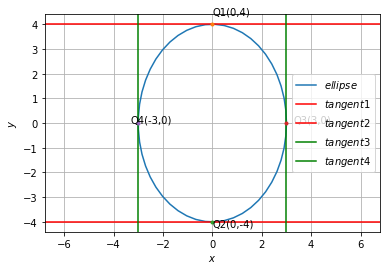
\includegraphics[width=\columnwidth]{./solutions/conics/1/16/ellipse.png}
	\caption{Figure depicting point of contact of tangents of ellipse parallel to x-axis and y-axis}
	\label{eq:solutions/1/16/fig1}
\end{figure}

%\subsection{Problem}
\item Triangles on the same base (or equal bases) and between the same parallels are equal in area.
\\
\solution

General equation of conics is 
\begin{align}
    \vec{x}^T\vec{V}\vec{x}+ 2\vec{u}^T\vec{x}+f = 0
    \label{eq:solutions/1/16/eq:1}
\end{align}
Comparing with the equation given,
\begin{align}
\vec{V}=\myvec{\frac{1}{9} & 0 \\ 0 & \frac{1}{16}}\\
\vec{u}=\vec{0}\\
f=-1\\
\mydet{\vec{v}}=\mydet{\myvec{\frac{1}{9} & 0 \\ 0 & \frac{1}{16}}}>0
\end{align}
$\because \abs{\vec{V}}>0$, the given equation is of ellipse.\\
a)The tangents are parallel to the x-axis, hence, their direction and normal vectors, $\vec{m_1}$ and $\vec{n_1}$ are respectively,
\begin{align}
\vec{m_1}=\myvec{1\\0}\\
\vec{n_1}=\myvec{0\\1}
\end{align}
For an ellipse, given the normal vector $\vec{n}$, the tangent points of contact to the ellipse are given by
\begin{align}
    \vec{q}=\vec{V}^{-1}(\kappa \vec{n}-\vec{u})
    \label{eq:solutions/1/16/eq:2}
    =\vec{V}^{-1}\kappa \vec{n}
\end{align}
where
\begin{align}
    \kappa=\pm \sqrt{\frac{\vec{u^T}\vec{V}^{-1}\vec{u}-f}{\vec{n^T}\vec{V}^{-1}\vec{n}}}
    \label{eq:solutions/1/16/eq:2.0.9}\\
   =\pm \sqrt{\frac{-f}{\vec{n^T}\vec{V}^{-1}\vec{n}}}\\
    \vec{V}^{-1}=\myvec{9 & 0 \\ 0 & 16}\\
    \kappa_1=\pm \sqrt{\frac{-(-1)}{\myvec{0 & 1}\myvec{9 & 0 \\ 0 & 16} \myvec{0\\1}}}\\
 \implies \kappa_1=\pm \sqrt{\frac{1}{16}}\\
    \implies \kappa_1=\pm \frac{1}{4}      
\end{align}
From \eqref{eq:solutions/1/16/eq:2} , the point of contact $\vec{q_i}$ are,
\begin{align}
    \vec{q_1}=\myvec{9 & 0 \\ 0 & 16}\frac{1}{4}\myvec{0\\1}\\
    =\myvec{9 & 0 \\ 0 & 16}\myvec{0\\\frac{1}{4}}\\
    =\myvec{0\\4}\\
    \vec{q_2}=\myvec{9 & 0 \\ 0 & 16}\left(-\frac{1}{4}\right)\ \myvec{0\\1}\\
    =\myvec{9 & 0 \\ 0 & 16}\myvec{0\\-\frac{1}{4}}\\
    =\myvec{0\\-4}
\end{align}
b) The tangents are parallel to the y-axis, hence, their direction and normal vectors, $\vec{m_2}$ and $\vec{n_2}$ are respectively,
\begin{align}
\vec{m_2}=\myvec{0\\1}\\
\vec{n_2}=\myvec{1\\0}
\end{align}
Using equation \eqref{eq:solutions/1/16/eq:2.0.9}, the values of $\kappa$ for this case are
\begin{align}
     \kappa_2=\pm \sqrt{\frac{-(-1)}{\myvec{1 & 0}\myvec{9 & 0 \\ 0 & 16} \myvec{1\\0}}}\\
 \implies \kappa_2=\pm \sqrt{\frac{1}{9}}\\
    \implies \kappa_2=\pm \frac{1}{3} 
\end{align}
and from \eqref{eq:solutions/1/16/eq:2} , the point of contact $\vec{q_i}$ are,
\begin{align}
\vec{q_3}=\myvec{9 & 0 \\ 0 & 16}\frac{1}{3}\myvec{1\\0}\\
    =\myvec{9 & 0 \\ 0 & 16}\myvec{\frac{1}{3}\\0}\\
    =\myvec{3\\0}\\
\vec{q_4}=\myvec{9 & 0 \\ 0 & 16}\left(-\frac{1}{3}\right)\ \myvec{1\\0}\\
    =\myvec{9 & 0 \\ 0 & 16}\myvec{-\frac{1}{3}\\0}\\
    =\myvec{-3\\0}
\end{align}
 \begin{figure}[h!]
	\centering
	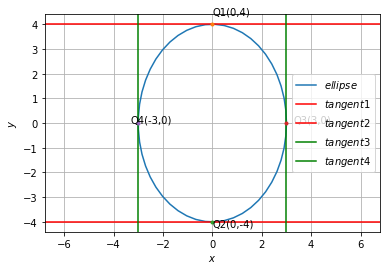
\includegraphics[width=\columnwidth]{./solutions/conics/1/16/ellipse.png}
	\caption{Figure depicting point of contact of tangents of ellipse parallel to x-axis and y-axis}
	\label{eq:solutions/1/16/fig1}
\end{figure}

\item Triangles on the same base (or equal bases) and having equal areas lie between the same parallels.
\\
\solution

General equation of conics is 
\begin{align}
    \vec{x}^T\vec{V}\vec{x}+ 2\vec{u}^T\vec{x}+f = 0
    \label{eq:solutions/1/16/eq:1}
\end{align}
Comparing with the equation given,
\begin{align}
\vec{V}=\myvec{\frac{1}{9} & 0 \\ 0 & \frac{1}{16}}\\
\vec{u}=\vec{0}\\
f=-1\\
\mydet{\vec{v}}=\mydet{\myvec{\frac{1}{9} & 0 \\ 0 & \frac{1}{16}}}>0
\end{align}
$\because \abs{\vec{V}}>0$, the given equation is of ellipse.\\
a)The tangents are parallel to the x-axis, hence, their direction and normal vectors, $\vec{m_1}$ and $\vec{n_1}$ are respectively,
\begin{align}
\vec{m_1}=\myvec{1\\0}\\
\vec{n_1}=\myvec{0\\1}
\end{align}
For an ellipse, given the normal vector $\vec{n}$, the tangent points of contact to the ellipse are given by
\begin{align}
    \vec{q}=\vec{V}^{-1}(\kappa \vec{n}-\vec{u})
    \label{eq:solutions/1/16/eq:2}
    =\vec{V}^{-1}\kappa \vec{n}
\end{align}
where
\begin{align}
    \kappa=\pm \sqrt{\frac{\vec{u^T}\vec{V}^{-1}\vec{u}-f}{\vec{n^T}\vec{V}^{-1}\vec{n}}}
    \label{eq:solutions/1/16/eq:2.0.9}\\
   =\pm \sqrt{\frac{-f}{\vec{n^T}\vec{V}^{-1}\vec{n}}}\\
    \vec{V}^{-1}=\myvec{9 & 0 \\ 0 & 16}\\
    \kappa_1=\pm \sqrt{\frac{-(-1)}{\myvec{0 & 1}\myvec{9 & 0 \\ 0 & 16} \myvec{0\\1}}}\\
 \implies \kappa_1=\pm \sqrt{\frac{1}{16}}\\
    \implies \kappa_1=\pm \frac{1}{4}      
\end{align}
From \eqref{eq:solutions/1/16/eq:2} , the point of contact $\vec{q_i}$ are,
\begin{align}
    \vec{q_1}=\myvec{9 & 0 \\ 0 & 16}\frac{1}{4}\myvec{0\\1}\\
    =\myvec{9 & 0 \\ 0 & 16}\myvec{0\\\frac{1}{4}}\\
    =\myvec{0\\4}\\
    \vec{q_2}=\myvec{9 & 0 \\ 0 & 16}\left(-\frac{1}{4}\right)\ \myvec{0\\1}\\
    =\myvec{9 & 0 \\ 0 & 16}\myvec{0\\-\frac{1}{4}}\\
    =\myvec{0\\-4}
\end{align}
b) The tangents are parallel to the y-axis, hence, their direction and normal vectors, $\vec{m_2}$ and $\vec{n_2}$ are respectively,
\begin{align}
\vec{m_2}=\myvec{0\\1}\\
\vec{n_2}=\myvec{1\\0}
\end{align}
Using equation \eqref{eq:solutions/1/16/eq:2.0.9}, the values of $\kappa$ for this case are
\begin{align}
     \kappa_2=\pm \sqrt{\frac{-(-1)}{\myvec{1 & 0}\myvec{9 & 0 \\ 0 & 16} \myvec{1\\0}}}\\
 \implies \kappa_2=\pm \sqrt{\frac{1}{9}}\\
    \implies \kappa_2=\pm \frac{1}{3} 
\end{align}
and from \eqref{eq:solutions/1/16/eq:2} , the point of contact $\vec{q_i}$ are,
\begin{align}
\vec{q_3}=\myvec{9 & 0 \\ 0 & 16}\frac{1}{3}\myvec{1\\0}\\
    =\myvec{9 & 0 \\ 0 & 16}\myvec{\frac{1}{3}\\0}\\
    =\myvec{3\\0}\\
\vec{q_4}=\myvec{9 & 0 \\ 0 & 16}\left(-\frac{1}{3}\right)\ \myvec{1\\0}\\
    =\myvec{9 & 0 \\ 0 & 16}\myvec{-\frac{1}{3}\\0}\\
    =\myvec{-3\\0}
\end{align}
 \begin{figure}[h!]
	\centering
	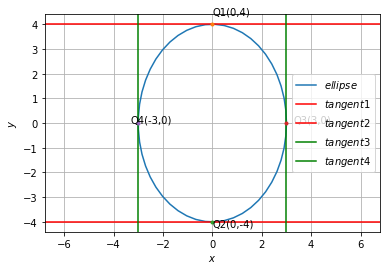
\includegraphics[width=\columnwidth]{./solutions/conics/1/16/ellipse.png}
	\caption{Figure depicting point of contact of tangents of ellipse parallel to x-axis and y-axis}
	\label{eq:solutions/1/16/fig1}
\end{figure}

\item In $\triangle ABC$, the bisector $AD$ of $\angle  A$ is perpendicular to side $BC$. Show that $AB = AC$ and $\triangle ABC$ is isosceles.
\\
\solution

General equation of conics is 
\begin{align}
    \vec{x}^T\vec{V}\vec{x}+ 2\vec{u}^T\vec{x}+f = 0
    \label{eq:solutions/1/16/eq:1}
\end{align}
Comparing with the equation given,
\begin{align}
\vec{V}=\myvec{\frac{1}{9} & 0 \\ 0 & \frac{1}{16}}\\
\vec{u}=\vec{0}\\
f=-1\\
\mydet{\vec{v}}=\mydet{\myvec{\frac{1}{9} & 0 \\ 0 & \frac{1}{16}}}>0
\end{align}
$\because \abs{\vec{V}}>0$, the given equation is of ellipse.\\
a)The tangents are parallel to the x-axis, hence, their direction and normal vectors, $\vec{m_1}$ and $\vec{n_1}$ are respectively,
\begin{align}
\vec{m_1}=\myvec{1\\0}\\
\vec{n_1}=\myvec{0\\1}
\end{align}
For an ellipse, given the normal vector $\vec{n}$, the tangent points of contact to the ellipse are given by
\begin{align}
    \vec{q}=\vec{V}^{-1}(\kappa \vec{n}-\vec{u})
    \label{eq:solutions/1/16/eq:2}
    =\vec{V}^{-1}\kappa \vec{n}
\end{align}
where
\begin{align}
    \kappa=\pm \sqrt{\frac{\vec{u^T}\vec{V}^{-1}\vec{u}-f}{\vec{n^T}\vec{V}^{-1}\vec{n}}}
    \label{eq:solutions/1/16/eq:2.0.9}\\
   =\pm \sqrt{\frac{-f}{\vec{n^T}\vec{V}^{-1}\vec{n}}}\\
    \vec{V}^{-1}=\myvec{9 & 0 \\ 0 & 16}\\
    \kappa_1=\pm \sqrt{\frac{-(-1)}{\myvec{0 & 1}\myvec{9 & 0 \\ 0 & 16} \myvec{0\\1}}}\\
 \implies \kappa_1=\pm \sqrt{\frac{1}{16}}\\
    \implies \kappa_1=\pm \frac{1}{4}      
\end{align}
From \eqref{eq:solutions/1/16/eq:2} , the point of contact $\vec{q_i}$ are,
\begin{align}
    \vec{q_1}=\myvec{9 & 0 \\ 0 & 16}\frac{1}{4}\myvec{0\\1}\\
    =\myvec{9 & 0 \\ 0 & 16}\myvec{0\\\frac{1}{4}}\\
    =\myvec{0\\4}\\
    \vec{q_2}=\myvec{9 & 0 \\ 0 & 16}\left(-\frac{1}{4}\right)\ \myvec{0\\1}\\
    =\myvec{9 & 0 \\ 0 & 16}\myvec{0\\-\frac{1}{4}}\\
    =\myvec{0\\-4}
\end{align}
b) The tangents are parallel to the y-axis, hence, their direction and normal vectors, $\vec{m_2}$ and $\vec{n_2}$ are respectively,
\begin{align}
\vec{m_2}=\myvec{0\\1}\\
\vec{n_2}=\myvec{1\\0}
\end{align}
Using equation \eqref{eq:solutions/1/16/eq:2.0.9}, the values of $\kappa$ for this case are
\begin{align}
     \kappa_2=\pm \sqrt{\frac{-(-1)}{\myvec{1 & 0}\myvec{9 & 0 \\ 0 & 16} \myvec{1\\0}}}\\
 \implies \kappa_2=\pm \sqrt{\frac{1}{9}}\\
    \implies \kappa_2=\pm \frac{1}{3} 
\end{align}
and from \eqref{eq:solutions/1/16/eq:2} , the point of contact $\vec{q_i}$ are,
\begin{align}
\vec{q_3}=\myvec{9 & 0 \\ 0 & 16}\frac{1}{3}\myvec{1\\0}\\
    =\myvec{9 & 0 \\ 0 & 16}\myvec{\frac{1}{3}\\0}\\
    =\myvec{3\\0}\\
\vec{q_4}=\myvec{9 & 0 \\ 0 & 16}\left(-\frac{1}{3}\right)\ \myvec{1\\0}\\
    =\myvec{9 & 0 \\ 0 & 16}\myvec{-\frac{1}{3}\\0}\\
    =\myvec{-3\\0}
\end{align}
 \begin{figure}[h!]
	\centering
	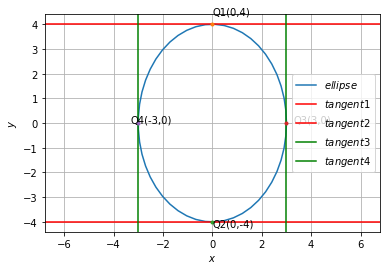
\includegraphics[width=\columnwidth]{./solutions/conics/1/16/ellipse.png}
	\caption{Figure depicting point of contact of tangents of ellipse parallel to x-axis and y-axis}
	\label{eq:solutions/1/16/fig1}
\end{figure}

\item $E$ and $F$ are respectively the mid-points of equal sides $AB$ and AC of $\triangle ABC$. Show that $BF = CE$. \\
\solution

General equation of conics is 
\begin{align}
    \vec{x}^T\vec{V}\vec{x}+ 2\vec{u}^T\vec{x}+f = 0
    \label{eq:solutions/1/16/eq:1}
\end{align}
Comparing with the equation given,
\begin{align}
\vec{V}=\myvec{\frac{1}{9} & 0 \\ 0 & \frac{1}{16}}\\
\vec{u}=\vec{0}\\
f=-1\\
\mydet{\vec{v}}=\mydet{\myvec{\frac{1}{9} & 0 \\ 0 & \frac{1}{16}}}>0
\end{align}
$\because \abs{\vec{V}}>0$, the given equation is of ellipse.\\
a)The tangents are parallel to the x-axis, hence, their direction and normal vectors, $\vec{m_1}$ and $\vec{n_1}$ are respectively,
\begin{align}
\vec{m_1}=\myvec{1\\0}\\
\vec{n_1}=\myvec{0\\1}
\end{align}
For an ellipse, given the normal vector $\vec{n}$, the tangent points of contact to the ellipse are given by
\begin{align}
    \vec{q}=\vec{V}^{-1}(\kappa \vec{n}-\vec{u})
    \label{eq:solutions/1/16/eq:2}
    =\vec{V}^{-1}\kappa \vec{n}
\end{align}
where
\begin{align}
    \kappa=\pm \sqrt{\frac{\vec{u^T}\vec{V}^{-1}\vec{u}-f}{\vec{n^T}\vec{V}^{-1}\vec{n}}}
    \label{eq:solutions/1/16/eq:2.0.9}\\
   =\pm \sqrt{\frac{-f}{\vec{n^T}\vec{V}^{-1}\vec{n}}}\\
    \vec{V}^{-1}=\myvec{9 & 0 \\ 0 & 16}\\
    \kappa_1=\pm \sqrt{\frac{-(-1)}{\myvec{0 & 1}\myvec{9 & 0 \\ 0 & 16} \myvec{0\\1}}}\\
 \implies \kappa_1=\pm \sqrt{\frac{1}{16}}\\
    \implies \kappa_1=\pm \frac{1}{4}      
\end{align}
From \eqref{eq:solutions/1/16/eq:2} , the point of contact $\vec{q_i}$ are,
\begin{align}
    \vec{q_1}=\myvec{9 & 0 \\ 0 & 16}\frac{1}{4}\myvec{0\\1}\\
    =\myvec{9 & 0 \\ 0 & 16}\myvec{0\\\frac{1}{4}}\\
    =\myvec{0\\4}\\
    \vec{q_2}=\myvec{9 & 0 \\ 0 & 16}\left(-\frac{1}{4}\right)\ \myvec{0\\1}\\
    =\myvec{9 & 0 \\ 0 & 16}\myvec{0\\-\frac{1}{4}}\\
    =\myvec{0\\-4}
\end{align}
b) The tangents are parallel to the y-axis, hence, their direction and normal vectors, $\vec{m_2}$ and $\vec{n_2}$ are respectively,
\begin{align}
\vec{m_2}=\myvec{0\\1}\\
\vec{n_2}=\myvec{1\\0}
\end{align}
Using equation \eqref{eq:solutions/1/16/eq:2.0.9}, the values of $\kappa$ for this case are
\begin{align}
     \kappa_2=\pm \sqrt{\frac{-(-1)}{\myvec{1 & 0}\myvec{9 & 0 \\ 0 & 16} \myvec{1\\0}}}\\
 \implies \kappa_2=\pm \sqrt{\frac{1}{9}}\\
    \implies \kappa_2=\pm \frac{1}{3} 
\end{align}
and from \eqref{eq:solutions/1/16/eq:2} , the point of contact $\vec{q_i}$ are,
\begin{align}
\vec{q_3}=\myvec{9 & 0 \\ 0 & 16}\frac{1}{3}\myvec{1\\0}\\
    =\myvec{9 & 0 \\ 0 & 16}\myvec{\frac{1}{3}\\0}\\
    =\myvec{3\\0}\\
\vec{q_4}=\myvec{9 & 0 \\ 0 & 16}\left(-\frac{1}{3}\right)\ \myvec{1\\0}\\
    =\myvec{9 & 0 \\ 0 & 16}\myvec{-\frac{1}{3}\\0}\\
    =\myvec{-3\\0}
\end{align}
 \begin{figure}[h!]
	\centering
	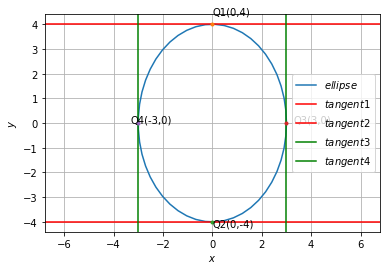
\includegraphics[width=\columnwidth]{./solutions/conics/1/16/ellipse.png}
	\caption{Figure depicting point of contact of tangents of ellipse parallel to x-axis and y-axis}
	\label{eq:solutions/1/16/fig1}
\end{figure}


\item In an isosceles $\triangle ABC$ with $AB$ = AC, D and E are points on $BC$ such that $BE = CD$. Show that $AD = AE$. 
%
\\
\solution

General equation of conics is 
\begin{align}
    \vec{x}^T\vec{V}\vec{x}+ 2\vec{u}^T\vec{x}+f = 0
    \label{eq:solutions/1/16/eq:1}
\end{align}
Comparing with the equation given,
\begin{align}
\vec{V}=\myvec{\frac{1}{9} & 0 \\ 0 & \frac{1}{16}}\\
\vec{u}=\vec{0}\\
f=-1\\
\mydet{\vec{v}}=\mydet{\myvec{\frac{1}{9} & 0 \\ 0 & \frac{1}{16}}}>0
\end{align}
$\because \abs{\vec{V}}>0$, the given equation is of ellipse.\\
a)The tangents are parallel to the x-axis, hence, their direction and normal vectors, $\vec{m_1}$ and $\vec{n_1}$ are respectively,
\begin{align}
\vec{m_1}=\myvec{1\\0}\\
\vec{n_1}=\myvec{0\\1}
\end{align}
For an ellipse, given the normal vector $\vec{n}$, the tangent points of contact to the ellipse are given by
\begin{align}
    \vec{q}=\vec{V}^{-1}(\kappa \vec{n}-\vec{u})
    \label{eq:solutions/1/16/eq:2}
    =\vec{V}^{-1}\kappa \vec{n}
\end{align}
where
\begin{align}
    \kappa=\pm \sqrt{\frac{\vec{u^T}\vec{V}^{-1}\vec{u}-f}{\vec{n^T}\vec{V}^{-1}\vec{n}}}
    \label{eq:solutions/1/16/eq:2.0.9}\\
   =\pm \sqrt{\frac{-f}{\vec{n^T}\vec{V}^{-1}\vec{n}}}\\
    \vec{V}^{-1}=\myvec{9 & 0 \\ 0 & 16}\\
    \kappa_1=\pm \sqrt{\frac{-(-1)}{\myvec{0 & 1}\myvec{9 & 0 \\ 0 & 16} \myvec{0\\1}}}\\
 \implies \kappa_1=\pm \sqrt{\frac{1}{16}}\\
    \implies \kappa_1=\pm \frac{1}{4}      
\end{align}
From \eqref{eq:solutions/1/16/eq:2} , the point of contact $\vec{q_i}$ are,
\begin{align}
    \vec{q_1}=\myvec{9 & 0 \\ 0 & 16}\frac{1}{4}\myvec{0\\1}\\
    =\myvec{9 & 0 \\ 0 & 16}\myvec{0\\\frac{1}{4}}\\
    =\myvec{0\\4}\\
    \vec{q_2}=\myvec{9 & 0 \\ 0 & 16}\left(-\frac{1}{4}\right)\ \myvec{0\\1}\\
    =\myvec{9 & 0 \\ 0 & 16}\myvec{0\\-\frac{1}{4}}\\
    =\myvec{0\\-4}
\end{align}
b) The tangents are parallel to the y-axis, hence, their direction and normal vectors, $\vec{m_2}$ and $\vec{n_2}$ are respectively,
\begin{align}
\vec{m_2}=\myvec{0\\1}\\
\vec{n_2}=\myvec{1\\0}
\end{align}
Using equation \eqref{eq:solutions/1/16/eq:2.0.9}, the values of $\kappa$ for this case are
\begin{align}
     \kappa_2=\pm \sqrt{\frac{-(-1)}{\myvec{1 & 0}\myvec{9 & 0 \\ 0 & 16} \myvec{1\\0}}}\\
 \implies \kappa_2=\pm \sqrt{\frac{1}{9}}\\
    \implies \kappa_2=\pm \frac{1}{3} 
\end{align}
and from \eqref{eq:solutions/1/16/eq:2} , the point of contact $\vec{q_i}$ are,
\begin{align}
\vec{q_3}=\myvec{9 & 0 \\ 0 & 16}\frac{1}{3}\myvec{1\\0}\\
    =\myvec{9 & 0 \\ 0 & 16}\myvec{\frac{1}{3}\\0}\\
    =\myvec{3\\0}\\
\vec{q_4}=\myvec{9 & 0 \\ 0 & 16}\left(-\frac{1}{3}\right)\ \myvec{1\\0}\\
    =\myvec{9 & 0 \\ 0 & 16}\myvec{-\frac{1}{3}\\0}\\
    =\myvec{-3\\0}
\end{align}
 \begin{figure}[h!]
	\centering
	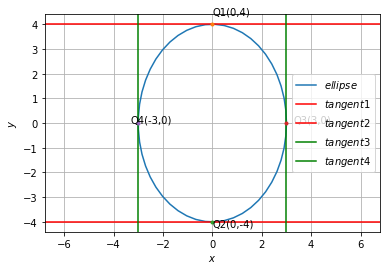
\includegraphics[width=\columnwidth]{./solutions/conics/1/16/ellipse.png}
	\caption{Figure depicting point of contact of tangents of ellipse parallel to x-axis and y-axis}
	\label{eq:solutions/1/16/fig1}
\end{figure}

%
\item $P$ is a point equidistant from two lines $l$ and $m$ intersecting at point $A$.  Show that the line  $AP$  bisects the angle between them.
%
\\
\solution

General equation of conics is 
\begin{align}
    \vec{x}^T\vec{V}\vec{x}+ 2\vec{u}^T\vec{x}+f = 0
    \label{eq:solutions/1/16/eq:1}
\end{align}
Comparing with the equation given,
\begin{align}
\vec{V}=\myvec{\frac{1}{9} & 0 \\ 0 & \frac{1}{16}}\\
\vec{u}=\vec{0}\\
f=-1\\
\mydet{\vec{v}}=\mydet{\myvec{\frac{1}{9} & 0 \\ 0 & \frac{1}{16}}}>0
\end{align}
$\because \abs{\vec{V}}>0$, the given equation is of ellipse.\\
a)The tangents are parallel to the x-axis, hence, their direction and normal vectors, $\vec{m_1}$ and $\vec{n_1}$ are respectively,
\begin{align}
\vec{m_1}=\myvec{1\\0}\\
\vec{n_1}=\myvec{0\\1}
\end{align}
For an ellipse, given the normal vector $\vec{n}$, the tangent points of contact to the ellipse are given by
\begin{align}
    \vec{q}=\vec{V}^{-1}(\kappa \vec{n}-\vec{u})
    \label{eq:solutions/1/16/eq:2}
    =\vec{V}^{-1}\kappa \vec{n}
\end{align}
where
\begin{align}
    \kappa=\pm \sqrt{\frac{\vec{u^T}\vec{V}^{-1}\vec{u}-f}{\vec{n^T}\vec{V}^{-1}\vec{n}}}
    \label{eq:solutions/1/16/eq:2.0.9}\\
   =\pm \sqrt{\frac{-f}{\vec{n^T}\vec{V}^{-1}\vec{n}}}\\
    \vec{V}^{-1}=\myvec{9 & 0 \\ 0 & 16}\\
    \kappa_1=\pm \sqrt{\frac{-(-1)}{\myvec{0 & 1}\myvec{9 & 0 \\ 0 & 16} \myvec{0\\1}}}\\
 \implies \kappa_1=\pm \sqrt{\frac{1}{16}}\\
    \implies \kappa_1=\pm \frac{1}{4}      
\end{align}
From \eqref{eq:solutions/1/16/eq:2} , the point of contact $\vec{q_i}$ are,
\begin{align}
    \vec{q_1}=\myvec{9 & 0 \\ 0 & 16}\frac{1}{4}\myvec{0\\1}\\
    =\myvec{9 & 0 \\ 0 & 16}\myvec{0\\\frac{1}{4}}\\
    =\myvec{0\\4}\\
    \vec{q_2}=\myvec{9 & 0 \\ 0 & 16}\left(-\frac{1}{4}\right)\ \myvec{0\\1}\\
    =\myvec{9 & 0 \\ 0 & 16}\myvec{0\\-\frac{1}{4}}\\
    =\myvec{0\\-4}
\end{align}
b) The tangents are parallel to the y-axis, hence, their direction and normal vectors, $\vec{m_2}$ and $\vec{n_2}$ are respectively,
\begin{align}
\vec{m_2}=\myvec{0\\1}\\
\vec{n_2}=\myvec{1\\0}
\end{align}
Using equation \eqref{eq:solutions/1/16/eq:2.0.9}, the values of $\kappa$ for this case are
\begin{align}
     \kappa_2=\pm \sqrt{\frac{-(-1)}{\myvec{1 & 0}\myvec{9 & 0 \\ 0 & 16} \myvec{1\\0}}}\\
 \implies \kappa_2=\pm \sqrt{\frac{1}{9}}\\
    \implies \kappa_2=\pm \frac{1}{3} 
\end{align}
and from \eqref{eq:solutions/1/16/eq:2} , the point of contact $\vec{q_i}$ are,
\begin{align}
\vec{q_3}=\myvec{9 & 0 \\ 0 & 16}\frac{1}{3}\myvec{1\\0}\\
    =\myvec{9 & 0 \\ 0 & 16}\myvec{\frac{1}{3}\\0}\\
    =\myvec{3\\0}\\
\vec{q_4}=\myvec{9 & 0 \\ 0 & 16}\left(-\frac{1}{3}\right)\ \myvec{1\\0}\\
    =\myvec{9 & 0 \\ 0 & 16}\myvec{-\frac{1}{3}\\0}\\
    =\myvec{-3\\0}
\end{align}
 \begin{figure}[h!]
	\centering
	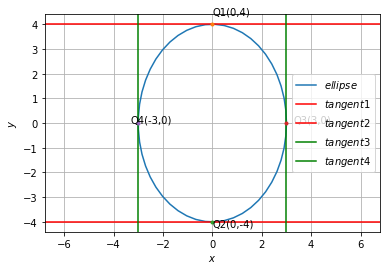
\includegraphics[width=\columnwidth]{./solutions/conics/1/16/ellipse.png}
	\caption{Figure depicting point of contact of tangents of ellipse parallel to x-axis and y-axis}
	\label{eq:solutions/1/16/fig1}
\end{figure}

\item $D$ is a point on side $BC$ of $\triangle  ABC$ such that $AD = AC$. Show that $AB > AD$
\\
\solution

General equation of conics is 
\begin{align}
    \vec{x}^T\vec{V}\vec{x}+ 2\vec{u}^T\vec{x}+f = 0
    \label{eq:solutions/1/16/eq:1}
\end{align}
Comparing with the equation given,
\begin{align}
\vec{V}=\myvec{\frac{1}{9} & 0 \\ 0 & \frac{1}{16}}\\
\vec{u}=\vec{0}\\
f=-1\\
\mydet{\vec{v}}=\mydet{\myvec{\frac{1}{9} & 0 \\ 0 & \frac{1}{16}}}>0
\end{align}
$\because \abs{\vec{V}}>0$, the given equation is of ellipse.\\
a)The tangents are parallel to the x-axis, hence, their direction and normal vectors, $\vec{m_1}$ and $\vec{n_1}$ are respectively,
\begin{align}
\vec{m_1}=\myvec{1\\0}\\
\vec{n_1}=\myvec{0\\1}
\end{align}
For an ellipse, given the normal vector $\vec{n}$, the tangent points of contact to the ellipse are given by
\begin{align}
    \vec{q}=\vec{V}^{-1}(\kappa \vec{n}-\vec{u})
    \label{eq:solutions/1/16/eq:2}
    =\vec{V}^{-1}\kappa \vec{n}
\end{align}
where
\begin{align}
    \kappa=\pm \sqrt{\frac{\vec{u^T}\vec{V}^{-1}\vec{u}-f}{\vec{n^T}\vec{V}^{-1}\vec{n}}}
    \label{eq:solutions/1/16/eq:2.0.9}\\
   =\pm \sqrt{\frac{-f}{\vec{n^T}\vec{V}^{-1}\vec{n}}}\\
    \vec{V}^{-1}=\myvec{9 & 0 \\ 0 & 16}\\
    \kappa_1=\pm \sqrt{\frac{-(-1)}{\myvec{0 & 1}\myvec{9 & 0 \\ 0 & 16} \myvec{0\\1}}}\\
 \implies \kappa_1=\pm \sqrt{\frac{1}{16}}\\
    \implies \kappa_1=\pm \frac{1}{4}      
\end{align}
From \eqref{eq:solutions/1/16/eq:2} , the point of contact $\vec{q_i}$ are,
\begin{align}
    \vec{q_1}=\myvec{9 & 0 \\ 0 & 16}\frac{1}{4}\myvec{0\\1}\\
    =\myvec{9 & 0 \\ 0 & 16}\myvec{0\\\frac{1}{4}}\\
    =\myvec{0\\4}\\
    \vec{q_2}=\myvec{9 & 0 \\ 0 & 16}\left(-\frac{1}{4}\right)\ \myvec{0\\1}\\
    =\myvec{9 & 0 \\ 0 & 16}\myvec{0\\-\frac{1}{4}}\\
    =\myvec{0\\-4}
\end{align}
b) The tangents are parallel to the y-axis, hence, their direction and normal vectors, $\vec{m_2}$ and $\vec{n_2}$ are respectively,
\begin{align}
\vec{m_2}=\myvec{0\\1}\\
\vec{n_2}=\myvec{1\\0}
\end{align}
Using equation \eqref{eq:solutions/1/16/eq:2.0.9}, the values of $\kappa$ for this case are
\begin{align}
     \kappa_2=\pm \sqrt{\frac{-(-1)}{\myvec{1 & 0}\myvec{9 & 0 \\ 0 & 16} \myvec{1\\0}}}\\
 \implies \kappa_2=\pm \sqrt{\frac{1}{9}}\\
    \implies \kappa_2=\pm \frac{1}{3} 
\end{align}
and from \eqref{eq:solutions/1/16/eq:2} , the point of contact $\vec{q_i}$ are,
\begin{align}
\vec{q_3}=\myvec{9 & 0 \\ 0 & 16}\frac{1}{3}\myvec{1\\0}\\
    =\myvec{9 & 0 \\ 0 & 16}\myvec{\frac{1}{3}\\0}\\
    =\myvec{3\\0}\\
\vec{q_4}=\myvec{9 & 0 \\ 0 & 16}\left(-\frac{1}{3}\right)\ \myvec{1\\0}\\
    =\myvec{9 & 0 \\ 0 & 16}\myvec{-\frac{1}{3}\\0}\\
    =\myvec{-3\\0}
\end{align}
 \begin{figure}[h!]
	\centering
	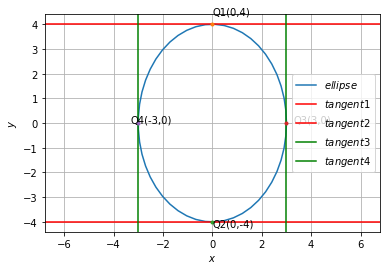
\includegraphics[width=\columnwidth]{./solutions/conics/1/16/ellipse.png}
	\caption{Figure depicting point of contact of tangents of ellipse parallel to x-axis and y-axis}
	\label{eq:solutions/1/16/fig1}
\end{figure}


%
\item $AB$ is a line segment and line $l$ is its perpendicular bisector. If a point $P$ lies on $l$, show that $P$ is equidistant from $A$ and $B$.
\\
\solution

General equation of conics is 
\begin{align}
    \vec{x}^T\vec{V}\vec{x}+ 2\vec{u}^T\vec{x}+f = 0
    \label{eq:solutions/1/16/eq:1}
\end{align}
Comparing with the equation given,
\begin{align}
\vec{V}=\myvec{\frac{1}{9} & 0 \\ 0 & \frac{1}{16}}\\
\vec{u}=\vec{0}\\
f=-1\\
\mydet{\vec{v}}=\mydet{\myvec{\frac{1}{9} & 0 \\ 0 & \frac{1}{16}}}>0
\end{align}
$\because \abs{\vec{V}}>0$, the given equation is of ellipse.\\
a)The tangents are parallel to the x-axis, hence, their direction and normal vectors, $\vec{m_1}$ and $\vec{n_1}$ are respectively,
\begin{align}
\vec{m_1}=\myvec{1\\0}\\
\vec{n_1}=\myvec{0\\1}
\end{align}
For an ellipse, given the normal vector $\vec{n}$, the tangent points of contact to the ellipse are given by
\begin{align}
    \vec{q}=\vec{V}^{-1}(\kappa \vec{n}-\vec{u})
    \label{eq:solutions/1/16/eq:2}
    =\vec{V}^{-1}\kappa \vec{n}
\end{align}
where
\begin{align}
    \kappa=\pm \sqrt{\frac{\vec{u^T}\vec{V}^{-1}\vec{u}-f}{\vec{n^T}\vec{V}^{-1}\vec{n}}}
    \label{eq:solutions/1/16/eq:2.0.9}\\
   =\pm \sqrt{\frac{-f}{\vec{n^T}\vec{V}^{-1}\vec{n}}}\\
    \vec{V}^{-1}=\myvec{9 & 0 \\ 0 & 16}\\
    \kappa_1=\pm \sqrt{\frac{-(-1)}{\myvec{0 & 1}\myvec{9 & 0 \\ 0 & 16} \myvec{0\\1}}}\\
 \implies \kappa_1=\pm \sqrt{\frac{1}{16}}\\
    \implies \kappa_1=\pm \frac{1}{4}      
\end{align}
From \eqref{eq:solutions/1/16/eq:2} , the point of contact $\vec{q_i}$ are,
\begin{align}
    \vec{q_1}=\myvec{9 & 0 \\ 0 & 16}\frac{1}{4}\myvec{0\\1}\\
    =\myvec{9 & 0 \\ 0 & 16}\myvec{0\\\frac{1}{4}}\\
    =\myvec{0\\4}\\
    \vec{q_2}=\myvec{9 & 0 \\ 0 & 16}\left(-\frac{1}{4}\right)\ \myvec{0\\1}\\
    =\myvec{9 & 0 \\ 0 & 16}\myvec{0\\-\frac{1}{4}}\\
    =\myvec{0\\-4}
\end{align}
b) The tangents are parallel to the y-axis, hence, their direction and normal vectors, $\vec{m_2}$ and $\vec{n_2}$ are respectively,
\begin{align}
\vec{m_2}=\myvec{0\\1}\\
\vec{n_2}=\myvec{1\\0}
\end{align}
Using equation \eqref{eq:solutions/1/16/eq:2.0.9}, the values of $\kappa$ for this case are
\begin{align}
     \kappa_2=\pm \sqrt{\frac{-(-1)}{\myvec{1 & 0}\myvec{9 & 0 \\ 0 & 16} \myvec{1\\0}}}\\
 \implies \kappa_2=\pm \sqrt{\frac{1}{9}}\\
    \implies \kappa_2=\pm \frac{1}{3} 
\end{align}
and from \eqref{eq:solutions/1/16/eq:2} , the point of contact $\vec{q_i}$ are,
\begin{align}
\vec{q_3}=\myvec{9 & 0 \\ 0 & 16}\frac{1}{3}\myvec{1\\0}\\
    =\myvec{9 & 0 \\ 0 & 16}\myvec{\frac{1}{3}\\0}\\
    =\myvec{3\\0}\\
\vec{q_4}=\myvec{9 & 0 \\ 0 & 16}\left(-\frac{1}{3}\right)\ \myvec{1\\0}\\
    =\myvec{9 & 0 \\ 0 & 16}\myvec{-\frac{1}{3}\\0}\\
    =\myvec{-3\\0}
\end{align}
 \begin{figure}[h!]
	\centering
	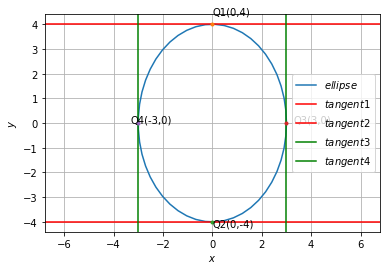
\includegraphics[width=\columnwidth]{./solutions/conics/1/16/ellipse.png}
	\caption{Figure depicting point of contact of tangents of ellipse parallel to x-axis and y-axis}
	\label{eq:solutions/1/16/fig1}
\end{figure}

\item Line-segment $AB$ is parallel to another line-segment $CD$. $O$ is the mid-point of $AD$. Show that 
\begin{enumerate}
\item  $\triangle AOB \cong \triangle DOC$ 
\item  $O$ is also the mid-point of $BC$.
\end{enumerate}
%
\item In quadrilateral $ACBD, AC = AD$ and $AB$ bisects $\angle  A$. Show that $\triangle  ABC \cong \triangle  ABD$. What can you say about $BC$ and $BD$?
\label{prob:8.1.23}
%\begin{enumerate}
%\renewcommand{\theequation}{\theenumi}
\begin{enumerate}[label=\thesection.\arabic*.,ref=\thesection.\theenumi]
\numberwithin{equation}{enumi}

\item The vertices of $\triangle ABC$ are taken as follows:
\label{const:table1}
\\
\solution See Table. \ref{table:table1} 
%
\begin{table}[ht!]
\centering
%%%%%%%%%%%%%%%%%%%%%%%%%%%%%%%%%%%%%%%%%%%%%%%%%%%%%%%%%%%%%%%%%%%%%%
%%                                                                  %%
%%  This is the header of a LaTeX2e file exported from Gnumeric.    %%
%%                                                                  %%
%%  This file can be compiled as it stands or included in another   %%
%%  LaTeX document. The table is based on the longtable package so  %%
%%  the longtable options (headers, footers...) can be set in the   %%
%%  preamble section below (see PRAMBLE).                           %%
%%                                                                  %%
%%  To include the file in another, the following two lines must be %%
%%  in the including file:                                          %%
%%        \def\inputGnumericTable{}                                 %%
%%  at the beginning of the file and:                               %%
%%        \input{name-of-this-file.tex}                             %%
%%  where the table is to be placed. Note also that the including   %%
%%  file must use the following packages for the table to be        %%
%%  rendered correctly:                                             %%
%%    \usepackage[latin1]{inputenc}                                 %%
%%    \usepackage{color}                                            %%
%%    \usepackage{array}                                            %%
%%    \usepackage{longtable}                                        %%
%%    \usepackage{calc}                                             %%
%%    \usepackage{multirow}                                         %%
%%    \usepackage{hhline}                                           %%
%%    \usepackage{ifthen}                                           %%
%%  optionally (for landscape tables embedded in another document): %%
%%    \usepackage{lscape}                                           %%
%%                                                                  %%
%%%%%%%%%%%%%%%%%%%%%%%%%%%%%%%%%%%%%%%%%%%%%%%%%%%%%%%%%%%%%%%%%%%%%%



%%  This section checks if we are begin input into another file or  %%
%%  the file will be compiled alone. First use a macro taken from   %%
%%  the TeXbook ex 7.7 (suggestion of Han-Wen Nienhuys).            %%
\def\ifundefined#1{\expandafter\ifx\csname#1\endcsname\relax}


%%  Check for the \def token for inputed files. If it is not        %%
%%  defined, the file will be processed as a standalone and the     %%
%%  preamble will be used.                                          %%
\ifundefined{inputGnumericTable}

%%  We must be able to close or not the document at the end.        %%
	\def\gnumericTableEnd{\end{document}}


%%%%%%%%%%%%%%%%%%%%%%%%%%%%%%%%%%%%%%%%%%%%%%%%%%%%%%%%%%%%%%%%%%%%%%
%%                                                                  %%
%%  This is the PREAMBLE. Change these values to get the right      %%
%%  paper size and other niceties.                                  %%
%%                                                                  %%
%%%%%%%%%%%%%%%%%%%%%%%%%%%%%%%%%%%%%%%%%%%%%%%%%%%%%%%%%%%%%%%%%%%%%%

	\documentclass[12pt%
			  %,landscape%
                    ]{report}
       \usepackage[latin1]{inputenc}
       \usepackage{fullpage}
       \usepackage{color}
       \usepackage{array}
       \usepackage{longtable}
       \usepackage{calc}
       \usepackage{multirow}
       \usepackage{hhline}
       \usepackage{ifthen}

	\begin{document}


%%  End of the preamble for the standalone. The next section is for %%
%%  documents which are included into other LaTeX2e files.          %%
\else

%%  We are not a stand alone document. For a regular table, we will %%
%%  have no preamble and only define the closing to mean nothing.   %%
    \def\gnumericTableEnd{}

%%  If we want landscape mode in an embedded document, comment out  %%
%%  the line above and uncomment the two below. The table will      %%
%%  begin on a new page and run in landscape mode.                  %%
%       \def\gnumericTableEnd{\end{landscape}}
%       \begin{landscape}


%%  End of the else clause for this file being \input.              %%
\fi

%%%%%%%%%%%%%%%%%%%%%%%%%%%%%%%%%%%%%%%%%%%%%%%%%%%%%%%%%%%%%%%%%%%%%%
%%                                                                  %%
%%  The rest is the gnumeric table, except for the closing          %%
%%  statement. Changes below will alter the table's appearance.     %%
%%                                                                  %%
%%%%%%%%%%%%%%%%%%%%%%%%%%%%%%%%%%%%%%%%%%%%%%%%%%%%%%%%%%%%%%%%%%%%%%

\providecommand{\gnumericmathit}[1]{#1} 
%%  Uncomment the next line if you would like your numbers to be in %%
%%  italics if they are italizised in the gnumeric table.           %%
%\renewcommand{\gnumericmathit}[1]{\mathit{#1}}
\providecommand{\gnumericPB}[1]%
{\let\gnumericTemp=\\#1\let\\=\gnumericTemp\hspace{0pt}}
 \ifundefined{gnumericTableWidthDefined}
        \newlength{\gnumericTableWidth}
        \newlength{\gnumericTableWidthComplete}
        \newlength{\gnumericMultiRowLength}
        \global\def\gnumericTableWidthDefined{}
 \fi
%% The following setting protects this code from babel shorthands.  %%
 \ifthenelse{\isundefined{\languageshorthands}}{}{\languageshorthands{english}}
%%  The default table format retains the relative column widths of  %%
%%  gnumeric. They can easily be changed to c, r or l. In that case %%
%%  you may want to comment out the next line and uncomment the one %%
%%  thereafter                                                      %%
\providecommand\gnumbox{\makebox[0pt]}
%%\providecommand\gnumbox[1][]{\makebox}

%% to adjust positions in multirow situations                       %%
\setlength{\bigstrutjot}{\jot}
\setlength{\extrarowheight}{\doublerulesep}

%%  The \setlongtables command keeps column widths the same across  %%
%%  pages. Simply comment out next line for varying column widths.  %%
\setlongtables

\setlength\gnumericTableWidth{%
	53pt+%
	53pt+%
0pt}
\def\gumericNumCols{2}
\setlength\gnumericTableWidthComplete{\gnumericTableWidth+%
         \tabcolsep*\gumericNumCols*2+\arrayrulewidth*\gumericNumCols}
\ifthenelse{\lengthtest{\gnumericTableWidthComplete > \linewidth}}%
         {\def\gnumericScale{\ratio{\linewidth-%
                        \tabcolsep*\gumericNumCols*2-%
                        \arrayrulewidth*\gumericNumCols}%
{\gnumericTableWidth}}}%
{\def\gnumericScale{1}}

%%%%%%%%%%%%%%%%%%%%%%%%%%%%%%%%%%%%%%%%%%%%%%%%%%%%%%%%%%%%%%%%%%%%%%
%%                                                                  %%
%% The following are the widths of the various columns. We are      %%
%% defining them here because then they are easier to change.       %%
%% Depending on the cell formats we may use them more than once.    %%
%%                                                                  %%
%%%%%%%%%%%%%%%%%%%%%%%%%%%%%%%%%%%%%%%%%%%%%%%%%%%%%%%%%%%%%%%%%%%%%%

\ifthenelse{\isundefined{\gnumericColA}}{\newlength{\gnumericColA}}{}\settowidth{\gnumericColA}{\begin{tabular}{@{}p{53pt*\gnumericScale}@{}}x\end{tabular}}
\ifthenelse{\isundefined{\gnumericColB}}{\newlength{\gnumericColB}}{}\settowidth{\gnumericColB}{\begin{tabular}{@{}p{53pt*\gnumericScale}@{}}x\end{tabular}}

\begin{tabular}[c]{%
	b{\gnumericColA}%
	b{\gnumericColB}%
	}

%%%%%%%%%%%%%%%%%%%%%%%%%%%%%%%%%%%%%%%%%%%%%%%%%%%%%%%%%%%%%%%%%%%%%%
%%  The longtable options. (Caption, headers... see Goosens, p.124) %%
%	\caption{The Table Caption.}             \\	%
% \hline	% Across the top of the table.
%%  The rest of these options are table rows which are placed on    %%
%%  the first, last or every page. Use \multicolumn if you want.    %%

%%  Header for the first page.                                      %%
%	\multicolumn{2}{c}{The First Header} \\ \hline 
%	\multicolumn{1}{c}{colTag}	%Column 1
%	&\multicolumn{1}{c}{colTag}	\\ \hline %Last column
%	\endfirsthead

%%  The running header definition.                                  %%
%	\hline
%	\multicolumn{2}{l}{\ldots\small\slshape continued} \\ \hline
%	\multicolumn{1}{c}{colTag}	%Column 1
%	&\multicolumn{1}{c}{colTag}	\\ \hline %Last column
%	\endhead

%%  The running footer definition.                                  %%
%	\hline
%	\multicolumn{2}{r}{\small\slshape continued\ldots} \\
%	\endfoot

%%  The ending footer definition.                                   %%
%	\multicolumn{2}{c}{That's all folks} \\ \hline 
%	\endlastfoot
%%%%%%%%%%%%%%%%%%%%%%%%%%%%%%%%%%%%%%%%%%%%%%%%%%%%%%%%%%%%%%%%%%%%%%

\hhline{|--}
	 \multicolumn{2}{|p{	\gnumericColA+%
	\gnumericColB+%
	\tabcolsep*2*1}|}%
	{\gnumericPB{\centering}\gnumbox{\textbf{Initial Input Values}}}
\\
\hhline{|-|-|}
	 \multicolumn{1}{|p{\gnumericColA}|}%
	{\gnumericPB{\centering}\gnumbox{\textbf{Parameter}}}
	&\multicolumn{1}{p{\gnumericColB}|}%
	{\gnumericPB{\centering}\gnumbox{\textbf{Value}}}
\\
\hhline{|--|}
	 \multicolumn{1}{|p{\gnumericColA}|}%
	{\gnumericPB{\centering}\gnumbox{\textbf{a}}}
	&\multicolumn{1}{p{\gnumericColB}|}%
	{\gnumericPB{\centering}\gnumbox{\textbf{4}}}
\\
\hhline{|--|}
	 \multicolumn{1}{|p{\gnumericColA}|}%
	{\gnumericPB{\centering}\gnumbox{\textbf{b}}}
	&\multicolumn{1}{p{\gnumericColB}|}%
	{\gnumericPB{\centering}\gnumbox{\textbf{4}}}
\\
\hhline{|--|}
	 \multicolumn{1}{|p{\gnumericColA}|}%
	{\gnumericPB{\centering}\gnumbox{\textbf{c}}}
	&\multicolumn{1}{p{\gnumericColB}|}%
	{\gnumericPB{\centering}\gnumbox{\textbf{4}}}
\\
\hhline{|-|-|}
\end{tabular}

\ifthenelse{\isundefined{\languageshorthands}}{}{\languageshorthands{\languagename}}
\gnumericTableEnd

\caption{To construct triangle ABC}
\label{table:table1}	
\end{table}

%\item

\item The midpoints of sides are given as
\begin{align}
\vec{D} &= \frac{\vec{B}+\vec{C}}{2}
\label{eq:pointd}
\\
\vec{E} &= \frac{\vec{A}+\vec{C}}{2}
\\
\vec{F} &= \frac{\vec{A}+\vec{B}}{2}
\end{align}
\item Also Centroid divides median in ratio 2:1.So by section formulae $\vec{O}$ is given as
\begin{align}
\vec{O} &= \frac{2\vec{D}+\vec{A}}{3}
\label{eq:centr}
\end{align}

The derived coordinates are listed in \ref{table:table2}. 
%
\begin{table}[ht!]
\centering
%%%%%%%%%%%%%%%%%%%%%%%%%%%%%%%%%%%%%%%%%%%%%%%%%%%%%%%%%%%%%%%%%%%%%%
%%                                                                  %%
%%  This is the header of a LaTeX2e file exported from Gnumeric.    %%
%%                                                                  %%
%%  This file can be compiled as it stands or included in another   %%
%%  LaTeX document. The table is based on the longtable package so  %%
%%  the longtable options (headers, footers...) can be set in the   %%
%%  preamble section below (see PRAMBLE).                           %%
%%                                                                  %%
%%  To include the file in another, the following two lines must be %%
%%  in the including file:                                          %%
%%        \def\inputGnumericTable{}                                 %%
%%  at the beginning of the file and:                               %%
%%        \input{name-of-this-file.tex}                             %%
%%  where the table is to be placed. Note also that the including   %%
%%  file must use the following packages for the table to be        %%
%%  rendered correctly:                                             %%
%%    \usepackage[latin1]{inputenc}                                 %%
%%    \usepackage{color}                                            %%
%%    \usepackage{array}                                            %%
%%    \usepackage{longtable}                                        %%
%%    \usepackage{calc}                                             %%
%%    \usepackage{multirow}                                         %%
%%    \usepackage{hhline}                                           %%
%%    \usepackage{ifthen}                                           %%
%%  optionally (for landscape tables embedded in another document): %%
%%    \usepackage{lscape}                                           %%
%%                                                                  %%
%%%%%%%%%%%%%%%%%%%%%%%%%%%%%%%%%%%%%%%%%%%%%%%%%%%%%%%%%%%%%%%%%%%%%%



%%  This section checks if we are begin input into another file or  %%
%%  the file will be compiled alone. First use a macro taken from   %%
%%  the TeXbook ex 7.7 (suggestion of Han-Wen Nienhuys).            %%
\def\ifundefined#1{\expandafter\ifx\csname#1\endcsname\relax}


%%  Check for the \def token for inputed files. If it is not        %%
%%  defined, the file will be processed as a standalone and the     %%
%%  preamble will be used.                                          %%
\ifundefined{inputGnumericTable}

%%  We must be able to close or not the document at the end.        %%
	\def\gnumericTableEnd{\end{document}}


%%%%%%%%%%%%%%%%%%%%%%%%%%%%%%%%%%%%%%%%%%%%%%%%%%%%%%%%%%%%%%%%%%%%%%
%%                                                                  %%
%%  This is the PREAMBLE. Change these values to get the right      %%
%%  paper size and other niceties.                                  %%
%%                                                                  %%
%%%%%%%%%%%%%%%%%%%%%%%%%%%%%%%%%%%%%%%%%%%%%%%%%%%%%%%%%%%%%%%%%%%%%%

	\documentclass[12pt%
			  %,landscape%
                    ]{report}
       \usepackage[latin1]{inputenc}
       \usepackage{fullpage}
       \usepackage{color}
       \usepackage{array}
       \usepackage{longtable}
       \usepackage{calc}
       \usepackage{multirow}
       \usepackage{hhline}
       \usepackage{ifthen}

	\begin{document}


%%  End of the preamble for the standalone. The next section is for %%
%%  documents which are included into other LaTeX2e files.          %%
\else

%%  We are not a stand alone document. For a regular table, we will %%
%%  have no preamble and only define the closing to mean nothing.   %%
    \def\gnumericTableEnd{}

%%  If we want landscape mode in an embedded document, comment out  %%
%%  the line above and uncomment the two below. The table will      %%
%%  begin on a new page and run in landscape mode.                  %%
%       \def\gnumericTableEnd{\end{landscape}}
%       \begin{landscape}


%%  End of the else clause for this file being \input.              %%
\fi

%%%%%%%%%%%%%%%%%%%%%%%%%%%%%%%%%%%%%%%%%%%%%%%%%%%%%%%%%%%%%%%%%%%%%%
%%                                                                  %%
%%  The rest is the gnumeric table, except for the closing          %%
%%  statement. Changes below will alter the table's appearance.     %%
%%                                                                  %%
%%%%%%%%%%%%%%%%%%%%%%%%%%%%%%%%%%%%%%%%%%%%%%%%%%%%%%%%%%%%%%%%%%%%%%

\providecommand{\gnumericmathit}[1]{#1} 
%%  Uncomment the next line if you would like your numbers to be in %%
%%  italics if they are italizised in the gnumeric table.           %%
%\renewcommand{\gnumericmathit}[1]{\mathit{#1}}
\providecommand{\gnumericPB}[1]%
{\let\gnumericTemp=\\#1\let\\=\gnumericTemp\hspace{0pt}}
 \ifundefined{gnumericTableWidthDefined}
        \newlength{\gnumericTableWidth}
        \newlength{\gnumericTableWidthComplete}
        \newlength{\gnumericMultiRowLength}
        \global\def\gnumericTableWidthDefined{}
 \fi
%% The following setting protects this code from babel shorthands.  %%
 \ifthenelse{\isundefined{\languageshorthands}}{}{\languageshorthands{english}}
%%  The default table format retains the relative column widths of  %%
%%  gnumeric. They can easily be changed to c, r or l. In that case %%
%%  you may want to comment out the next line and uncomment the one %%
%%  thereafter                                                      %%
\providecommand\gnumbox{\makebox[0pt]}
%%\providecommand\gnumbox[1][]{\makebox}

%% to adjust positions in multirow situations                       %%
\setlength{\bigstrutjot}{\jot}
\setlength{\extrarowheight}{\doublerulesep}

%%  The \setlongtables command keeps column widths the same across  %%
%%  pages. Simply comment out next line for varying column widths.  %%
\setlongtables

\setlength\gnumericTableWidth{%
	50pt+%
	75pt+%
0pt}
\def\gumericNumCols{2}
\setlength\gnumericTableWidthComplete{\gnumericTableWidth+%
         \tabcolsep*\gumericNumCols*2+\arrayrulewidth*\gumericNumCols}
\ifthenelse{\lengthtest{\gnumericTableWidthComplete > \linewidth}}%
         {\def\gnumericScale{\ratio{\linewidth-%
                        \tabcolsep*\gumericNumCols*2-%
                        \arrayrulewidth*\gumericNumCols}%
{\gnumericTableWidth}}}%
{\def\gnumericScale{1}}

%%%%%%%%%%%%%%%%%%%%%%%%%%%%%%%%%%%%%%%%%%%%%%%%%%%%%%%%%%%%%%%%%%%%%%
%%                                                                  %%
%% The following are the widths of the various columns. We are      %%
%% defining them here because then they are easier to change.       %%
%% Depending on the cell formats we may use them more than once.    %%
%%                                                                  %%
%%%%%%%%%%%%%%%%%%%%%%%%%%%%%%%%%%%%%%%%%%%%%%%%%%%%%%%%%%%%%%%%%%%%%%

\ifthenelse{\isundefined{\gnumericColA}}{\newlength{\gnumericColA}}{}\settowidth{\gnumericColA}{\begin{tabular}{@{}p{50pt*\gnumericScale}@{}}x\end{tabular}}
\ifthenelse{\isundefined{\gnumericColB}}{\newlength{\gnumericColB}}{}\settowidth{\gnumericColB}{\begin{tabular}{@{}p{75pt*\gnumericScale}@{}}x\end{tabular}}

\begin{tabular}[c]{%
	b{\gnumericColA}%
	b{\gnumericColB}%
	}

%%%%%%%%%%%%%%%%%%%%%%%%%%%%%%%%%%%%%%%%%%%%%%%%%%%%%%%%%%%%%%%%%%%%%%
%%  The longtable options. (Caption, headers... see Goosens, p.124) %%
%	\caption{The Table Caption.}             \\	%
% \hline	% Across the top of the table.
%%  The rest of these options are table rows which are placed on    %%
%%  the first, last or every page. Use \multicolumn if you want.    %%

%%  Header for the first page.                                      %%
%	\multicolumn{2}{c}{The First Header} \\ \hline 
%	\multicolumn{1}{c}{colTag}	%Column 1
%	&\multicolumn{1}{c}{colTag}	\\ \hline %Last column
%	\endfirsthead

%%  The running header definition.                                  %%
%	\hline
%	\multicolumn{2}{l}{\ldots\small\slshape continued} \\ \hline
%	\multicolumn{1}{c}{colTag}	%Column 1
%	&\multicolumn{1}{c}{colTag}	\\ \hline %Last column
%	\endhead

%%  The running footer definition.                                  %%
%	\hline
%	\multicolumn{2}{r}{\small\slshape continued\ldots} \\
%	\endfoot

%%  The ending footer definition.                                   %%
%	\multicolumn{2}{c}{That's all folks} \\ \hline 
%	\endlastfoot
%%%%%%%%%%%%%%%%%%%%%%%%%%%%%%%%%%%%%%%%%%%%%%%%%%%%%%%%%%%%%%%%%%%%%%

\hhline{|-|-}
	 \multicolumn{1}{|p{\gnumericColA}|}%
	{\gnumericPB{\raggedright}\gnumbox[l]{Vector}}
	&\multicolumn{1}{p{\gnumericColB}|}%
	{\gnumericPB{\raggedright}\gnumbox[l]{Coordinates}}
\\
\hhline{|--|}
	 \multicolumn{1}{|p{\gnumericColA}|}%
	{\gnumericPB{\centering}\gnumbox{\textbf{D}}}
	&\multicolumn{1}{p{\gnumericColB}|}%
	{\gnumericPB{\centering}\gnumbox{$\myvec{3\\1}$}}
\\
\hhline{|--|}
	 \multicolumn{1}{|p{\gnumericColA}|}%
	{\gnumericPB{\centering}\gnumbox{\textbf{E}}}
	&\multicolumn{1}{p{\gnumericColB}|}%
	{\gnumericPB{\centering}\gnumbox{$\myvec{2\\0}$}}
\\
\hhline{|--|}
	 \multicolumn{1}{|p{\gnumericColA}|}%
	{\gnumericPB{\centering}\gnumbox{\textbf{F}}}
	&\multicolumn{1}{p{\gnumericColB}|}%
	{\gnumericPB{\centering}\gnumbox{$\myvec{1\\1}$}}
\\
\hhline{|--|}
	 \multicolumn{1}{|p{\gnumericColA}|}%
	{\gnumericPB{\centering}\gnumbox{\textbf{O}}}
	&\multicolumn{1}{p{\gnumericColB}|}%
	{\gnumericPB{\centering}\gnumbox{$\myvec{3\\\frac{2}{3}}$}}
\\
\hhline{|-|-|}
\end{tabular}

\ifthenelse{\isundefined{\languageshorthands}}{}{\languageshorthands{\languagename}}
\gnumericTableEnd

\caption{Derived coordinates of triangle ABC}
\label{table:table2}	
\end{table}

\end{enumerate}

%
General equation of conics is 
\begin{align}
    \vec{x}^T\vec{V}\vec{x}+ 2\vec{u}^T\vec{x}+f = 0
    \label{eq:solutions/1/16/eq:1}
\end{align}
Comparing with the equation given,
\begin{align}
\vec{V}=\myvec{\frac{1}{9} & 0 \\ 0 & \frac{1}{16}}\\
\vec{u}=\vec{0}\\
f=-1\\
\mydet{\vec{v}}=\mydet{\myvec{\frac{1}{9} & 0 \\ 0 & \frac{1}{16}}}>0
\end{align}
$\because \abs{\vec{V}}>0$, the given equation is of ellipse.\\
a)The tangents are parallel to the x-axis, hence, their direction and normal vectors, $\vec{m_1}$ and $\vec{n_1}$ are respectively,
\begin{align}
\vec{m_1}=\myvec{1\\0}\\
\vec{n_1}=\myvec{0\\1}
\end{align}
For an ellipse, given the normal vector $\vec{n}$, the tangent points of contact to the ellipse are given by
\begin{align}
    \vec{q}=\vec{V}^{-1}(\kappa \vec{n}-\vec{u})
    \label{eq:solutions/1/16/eq:2}
    =\vec{V}^{-1}\kappa \vec{n}
\end{align}
where
\begin{align}
    \kappa=\pm \sqrt{\frac{\vec{u^T}\vec{V}^{-1}\vec{u}-f}{\vec{n^T}\vec{V}^{-1}\vec{n}}}
    \label{eq:solutions/1/16/eq:2.0.9}\\
   =\pm \sqrt{\frac{-f}{\vec{n^T}\vec{V}^{-1}\vec{n}}}\\
    \vec{V}^{-1}=\myvec{9 & 0 \\ 0 & 16}\\
    \kappa_1=\pm \sqrt{\frac{-(-1)}{\myvec{0 & 1}\myvec{9 & 0 \\ 0 & 16} \myvec{0\\1}}}\\
 \implies \kappa_1=\pm \sqrt{\frac{1}{16}}\\
    \implies \kappa_1=\pm \frac{1}{4}      
\end{align}
From \eqref{eq:solutions/1/16/eq:2} , the point of contact $\vec{q_i}$ are,
\begin{align}
    \vec{q_1}=\myvec{9 & 0 \\ 0 & 16}\frac{1}{4}\myvec{0\\1}\\
    =\myvec{9 & 0 \\ 0 & 16}\myvec{0\\\frac{1}{4}}\\
    =\myvec{0\\4}\\
    \vec{q_2}=\myvec{9 & 0 \\ 0 & 16}\left(-\frac{1}{4}\right)\ \myvec{0\\1}\\
    =\myvec{9 & 0 \\ 0 & 16}\myvec{0\\-\frac{1}{4}}\\
    =\myvec{0\\-4}
\end{align}
b) The tangents are parallel to the y-axis, hence, their direction and normal vectors, $\vec{m_2}$ and $\vec{n_2}$ are respectively,
\begin{align}
\vec{m_2}=\myvec{0\\1}\\
\vec{n_2}=\myvec{1\\0}
\end{align}
Using equation \eqref{eq:solutions/1/16/eq:2.0.9}, the values of $\kappa$ for this case are
\begin{align}
     \kappa_2=\pm \sqrt{\frac{-(-1)}{\myvec{1 & 0}\myvec{9 & 0 \\ 0 & 16} \myvec{1\\0}}}\\
 \implies \kappa_2=\pm \sqrt{\frac{1}{9}}\\
    \implies \kappa_2=\pm \frac{1}{3} 
\end{align}
and from \eqref{eq:solutions/1/16/eq:2} , the point of contact $\vec{q_i}$ are,
\begin{align}
\vec{q_3}=\myvec{9 & 0 \\ 0 & 16}\frac{1}{3}\myvec{1\\0}\\
    =\myvec{9 & 0 \\ 0 & 16}\myvec{\frac{1}{3}\\0}\\
    =\myvec{3\\0}\\
\vec{q_4}=\myvec{9 & 0 \\ 0 & 16}\left(-\frac{1}{3}\right)\ \myvec{1\\0}\\
    =\myvec{9 & 0 \\ 0 & 16}\myvec{-\frac{1}{3}\\0}\\
    =\myvec{-3\\0}
\end{align}
 \begin{figure}[h!]
	\centering
	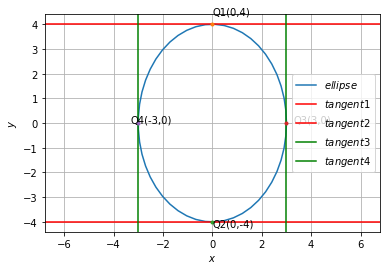
\includegraphics[width=\columnwidth]{./solutions/conics/1/16/ellipse.png}
	\caption{Figure depicting point of contact of tangents of ellipse parallel to x-axis and y-axis}
	\label{eq:solutions/1/16/fig1}
\end{figure}

%\end{enumerate}

%
\item $ABCD$ is a quadrilateral in which $AD = BC$ and $\angle  DAB = \angle  CBA$ . Prove that
\begin{enumerate}
\item  $\triangle  ABD \cong  \triangle  BAC $
\item $ BD = AC $
\item  $\angle  ABD = \angle  BAC$.
\end{enumerate}
%
\solution

General equation of conics is 
\begin{align}
    \vec{x}^T\vec{V}\vec{x}+ 2\vec{u}^T\vec{x}+f = 0
    \label{eq:solutions/1/16/eq:1}
\end{align}
Comparing with the equation given,
\begin{align}
\vec{V}=\myvec{\frac{1}{9} & 0 \\ 0 & \frac{1}{16}}\\
\vec{u}=\vec{0}\\
f=-1\\
\mydet{\vec{v}}=\mydet{\myvec{\frac{1}{9} & 0 \\ 0 & \frac{1}{16}}}>0
\end{align}
$\because \abs{\vec{V}}>0$, the given equation is of ellipse.\\
a)The tangents are parallel to the x-axis, hence, their direction and normal vectors, $\vec{m_1}$ and $\vec{n_1}$ are respectively,
\begin{align}
\vec{m_1}=\myvec{1\\0}\\
\vec{n_1}=\myvec{0\\1}
\end{align}
For an ellipse, given the normal vector $\vec{n}$, the tangent points of contact to the ellipse are given by
\begin{align}
    \vec{q}=\vec{V}^{-1}(\kappa \vec{n}-\vec{u})
    \label{eq:solutions/1/16/eq:2}
    =\vec{V}^{-1}\kappa \vec{n}
\end{align}
where
\begin{align}
    \kappa=\pm \sqrt{\frac{\vec{u^T}\vec{V}^{-1}\vec{u}-f}{\vec{n^T}\vec{V}^{-1}\vec{n}}}
    \label{eq:solutions/1/16/eq:2.0.9}\\
   =\pm \sqrt{\frac{-f}{\vec{n^T}\vec{V}^{-1}\vec{n}}}\\
    \vec{V}^{-1}=\myvec{9 & 0 \\ 0 & 16}\\
    \kappa_1=\pm \sqrt{\frac{-(-1)}{\myvec{0 & 1}\myvec{9 & 0 \\ 0 & 16} \myvec{0\\1}}}\\
 \implies \kappa_1=\pm \sqrt{\frac{1}{16}}\\
    \implies \kappa_1=\pm \frac{1}{4}      
\end{align}
From \eqref{eq:solutions/1/16/eq:2} , the point of contact $\vec{q_i}$ are,
\begin{align}
    \vec{q_1}=\myvec{9 & 0 \\ 0 & 16}\frac{1}{4}\myvec{0\\1}\\
    =\myvec{9 & 0 \\ 0 & 16}\myvec{0\\\frac{1}{4}}\\
    =\myvec{0\\4}\\
    \vec{q_2}=\myvec{9 & 0 \\ 0 & 16}\left(-\frac{1}{4}\right)\ \myvec{0\\1}\\
    =\myvec{9 & 0 \\ 0 & 16}\myvec{0\\-\frac{1}{4}}\\
    =\myvec{0\\-4}
\end{align}
b) The tangents are parallel to the y-axis, hence, their direction and normal vectors, $\vec{m_2}$ and $\vec{n_2}$ are respectively,
\begin{align}
\vec{m_2}=\myvec{0\\1}\\
\vec{n_2}=\myvec{1\\0}
\end{align}
Using equation \eqref{eq:solutions/1/16/eq:2.0.9}, the values of $\kappa$ for this case are
\begin{align}
     \kappa_2=\pm \sqrt{\frac{-(-1)}{\myvec{1 & 0}\myvec{9 & 0 \\ 0 & 16} \myvec{1\\0}}}\\
 \implies \kappa_2=\pm \sqrt{\frac{1}{9}}\\
    \implies \kappa_2=\pm \frac{1}{3} 
\end{align}
and from \eqref{eq:solutions/1/16/eq:2} , the point of contact $\vec{q_i}$ are,
\begin{align}
\vec{q_3}=\myvec{9 & 0 \\ 0 & 16}\frac{1}{3}\myvec{1\\0}\\
    =\myvec{9 & 0 \\ 0 & 16}\myvec{\frac{1}{3}\\0}\\
    =\myvec{3\\0}\\
\vec{q_4}=\myvec{9 & 0 \\ 0 & 16}\left(-\frac{1}{3}\right)\ \myvec{1\\0}\\
    =\myvec{9 & 0 \\ 0 & 16}\myvec{-\frac{1}{3}\\0}\\
    =\myvec{-3\\0}
\end{align}
 \begin{figure}[h!]
	\centering
	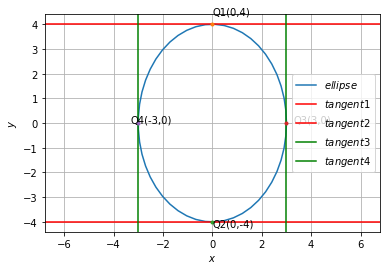
\includegraphics[width=\columnwidth]{./solutions/conics/1/16/ellipse.png}
	\caption{Figure depicting point of contact of tangents of ellipse parallel to x-axis and y-axis}
	\label{eq:solutions/1/16/fig1}
\end{figure}

\item $l$ and $m$ are two parallel lines intersected by another pair of parallel lines p and q 
to form the quadrilateral $ABCD$. Show that $\triangle  ABC \cong  \triangle  CDA$.
%
\item Line $l$ is the bisector of $ \angle  A$ and $B$ is any point on $l$. $BP$ and $BQ$ are perpendiculars from $B$ to the arms of $\angle  A$. Show that: 
\begin{enumerate}
\item  $\triangle  APB \cong  \triangle  AQB$ 
\item  $BP = BQ$ or $B$ is equidistant from the arms of $\angle  A$.
\end{enumerate}
\solution

General equation of conics is 
\begin{align}
    \vec{x}^T\vec{V}\vec{x}+ 2\vec{u}^T\vec{x}+f = 0
    \label{eq:solutions/1/16/eq:1}
\end{align}
Comparing with the equation given,
\begin{align}
\vec{V}=\myvec{\frac{1}{9} & 0 \\ 0 & \frac{1}{16}}\\
\vec{u}=\vec{0}\\
f=-1\\
\mydet{\vec{v}}=\mydet{\myvec{\frac{1}{9} & 0 \\ 0 & \frac{1}{16}}}>0
\end{align}
$\because \abs{\vec{V}}>0$, the given equation is of ellipse.\\
a)The tangents are parallel to the x-axis, hence, their direction and normal vectors, $\vec{m_1}$ and $\vec{n_1}$ are respectively,
\begin{align}
\vec{m_1}=\myvec{1\\0}\\
\vec{n_1}=\myvec{0\\1}
\end{align}
For an ellipse, given the normal vector $\vec{n}$, the tangent points of contact to the ellipse are given by
\begin{align}
    \vec{q}=\vec{V}^{-1}(\kappa \vec{n}-\vec{u})
    \label{eq:solutions/1/16/eq:2}
    =\vec{V}^{-1}\kappa \vec{n}
\end{align}
where
\begin{align}
    \kappa=\pm \sqrt{\frac{\vec{u^T}\vec{V}^{-1}\vec{u}-f}{\vec{n^T}\vec{V}^{-1}\vec{n}}}
    \label{eq:solutions/1/16/eq:2.0.9}\\
   =\pm \sqrt{\frac{-f}{\vec{n^T}\vec{V}^{-1}\vec{n}}}\\
    \vec{V}^{-1}=\myvec{9 & 0 \\ 0 & 16}\\
    \kappa_1=\pm \sqrt{\frac{-(-1)}{\myvec{0 & 1}\myvec{9 & 0 \\ 0 & 16} \myvec{0\\1}}}\\
 \implies \kappa_1=\pm \sqrt{\frac{1}{16}}\\
    \implies \kappa_1=\pm \frac{1}{4}      
\end{align}
From \eqref{eq:solutions/1/16/eq:2} , the point of contact $\vec{q_i}$ are,
\begin{align}
    \vec{q_1}=\myvec{9 & 0 \\ 0 & 16}\frac{1}{4}\myvec{0\\1}\\
    =\myvec{9 & 0 \\ 0 & 16}\myvec{0\\\frac{1}{4}}\\
    =\myvec{0\\4}\\
    \vec{q_2}=\myvec{9 & 0 \\ 0 & 16}\left(-\frac{1}{4}\right)\ \myvec{0\\1}\\
    =\myvec{9 & 0 \\ 0 & 16}\myvec{0\\-\frac{1}{4}}\\
    =\myvec{0\\-4}
\end{align}
b) The tangents are parallel to the y-axis, hence, their direction and normal vectors, $\vec{m_2}$ and $\vec{n_2}$ are respectively,
\begin{align}
\vec{m_2}=\myvec{0\\1}\\
\vec{n_2}=\myvec{1\\0}
\end{align}
Using equation \eqref{eq:solutions/1/16/eq:2.0.9}, the values of $\kappa$ for this case are
\begin{align}
     \kappa_2=\pm \sqrt{\frac{-(-1)}{\myvec{1 & 0}\myvec{9 & 0 \\ 0 & 16} \myvec{1\\0}}}\\
 \implies \kappa_2=\pm \sqrt{\frac{1}{9}}\\
    \implies \kappa_2=\pm \frac{1}{3} 
\end{align}
and from \eqref{eq:solutions/1/16/eq:2} , the point of contact $\vec{q_i}$ are,
\begin{align}
\vec{q_3}=\myvec{9 & 0 \\ 0 & 16}\frac{1}{3}\myvec{1\\0}\\
    =\myvec{9 & 0 \\ 0 & 16}\myvec{\frac{1}{3}\\0}\\
    =\myvec{3\\0}\\
\vec{q_4}=\myvec{9 & 0 \\ 0 & 16}\left(-\frac{1}{3}\right)\ \myvec{1\\0}\\
    =\myvec{9 & 0 \\ 0 & 16}\myvec{-\frac{1}{3}\\0}\\
    =\myvec{-3\\0}
\end{align}
 \begin{figure}[h!]
	\centering
	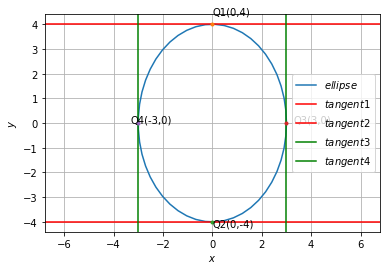
\includegraphics[width=\columnwidth]{./solutions/conics/1/16/ellipse.png}
	\caption{Figure depicting point of contact of tangents of ellipse parallel to x-axis and y-axis}
	\label{eq:solutions/1/16/fig1}
\end{figure}

%
%\begin{enumerate}
%
%\renewcommand{\thefigure}{\theenumi.\arabic{figure}}
\begin{figure}[!ht]
\centering
\resizebox{\columnwidth}{!}{\renewcommand{\theequation}{\theenumi}
\begin{enumerate}[label=\thesection.\arabic*.,ref=\thesection.\theenumi]
\numberwithin{equation}{enumi}
\item  Find the centre and radius of the circle 
\begin{align}
x^2+y^2+8x+10y-8 = 0
\label{eq:circ_basic}
\end{align}
\solution
\eqref{eq:circ_basic} can be expressed as 
\begin{align}
\vec{x}^T\vec{x}+ 2\myvec{4 & 5}\vec{x} -8 = 0
\end{align}
which is of the form \eqref{eq:conic_quad_form} with
\begin{align}
\label{eq:circ_basic_uf}
\vec{u} = \myvec{4\\5}, f = -8
\end{align}
From  Table \ref{table:conics}, the center and radius are given by 
\begin{align}
\vec{c} = -\vec{u} = \myvec{-4\\-5},
r = \sqrt{\norm{u}^2-f} = 7
\end{align}
\item Find the equation of a circle which passes through the points $\vec{P} = \myvec{2\\-2}$ and $\vec{Q} = \myvec{3\\4}$ and whose centre lies on the line  
%\cite{eleven}
\begin{align}
\label{eq:circ_ex1_line}
\myvec{1 & 1} \vec{x} = 2
\end{align}
\solution From \eqref{eq:conic_quad_form} and Table \ref{table:conics}, the equation of a circle can be expressed as
\begin{align}
\label{eq:circ_conic}
\vec{x}^T\vec{x}-2\vec{c}^T\vec{x}+f = 0
\end{align}
where $\vec{c}$ is the centre.
Substituting the given points in 
\eqref{eq:circ_conic} and using 
\eqref{eq:circ_ex1_line}, the following equations are obtained
\begin{align}
2\myvec{2 & -2}\vec{c} -  f &= 8
\\
2\myvec{3 & 4}\vec{c} -  f &= 25
\\
\myvec{1 & 1}\vec{c}  &= 2
\end{align}
which can be expressed as the matrix equation
\begin{align}
\myvec{
1 & 1 & 0
\\
4 & -4 & -1 
\\ 
6 & 8 & -1  
}
\myvec{\vec{c}\\f} = \myvec{2\\8\\25}
\end{align}
Row reducing the augmented matrix
\begin{align}
\myvec{
1 & 1 & 0 & 2
\\
4 & -4 & -1 & 8
\\ 
6 & 8 & -1  & 25
}
\\
\xleftrightarrow[R_3 \leftarrow R_3 -6R_1]{R_2 \leftarrow -R_2+4R_1}
\myvec{
1 & 1 & 0 & 2
\\
0 & 8 & 1 & 0
\\ 
0 & 2 & -1  & 13
}
\\
\xleftrightarrow[R_3 \leftarrow -\frac{4R_3 -R_2}{2}]{R_1 \leftarrow 8R_1-R_3}
\myvec{
8 & 0 & -1 & 16
\\
0 & 8 & 1 & 0
\\ 
0 & 0 & 5  & -52
}
\\
\xleftrightarrow[R_2 \leftarrow \frac{5R_2 -R_3}{4}]{R_1 \leftarrow \frac{5R_1+R_3}{4}}
\myvec{
10 & 0 & 0 & 7
\\
0 & 10 & 0 & 13
\\ 
0 & 0 & 5  & -52
}
\end{align}
Thus, 
\begin{align}
\vec{c} &= \frac{1}{10}\myvec{7\\13}
\\
f &=-\frac{52}{5}
\end{align}
which give the desired equation of the circle.
From Table \ref{table:conics},
%
\begin{align}
 r =  \sqrt{\norm{\vec{c}}^2-f} = \frac{1}{10}\sqrt{1258}
\end{align}
Fig. \ref{fig:CircOr}	verifies the above results.

\begin{figure}[!ht]
\centering
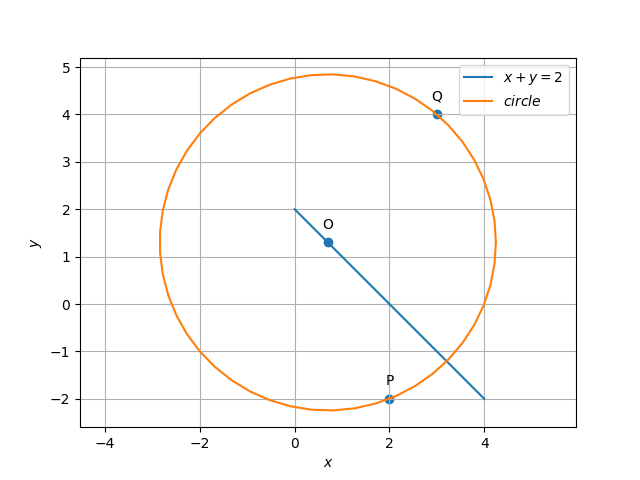
\includegraphics[width=\columnwidth]{./figs/circex/CircOr.eps}
\caption{Circle passing through $\myvec{2\\-2},\myvec{3\\4}$. Center is on line $\myvec{1 & 1}\vec{x}=2$. }
\label{fig:CircOr}	
\end{figure}

\item 
Find the points on the curve  
%\cite{twelve_one}
\begin{align}
x^2+y^2-2x-3 = 0
\label{eq:circle_tangent_prob}
\end{align}
at which the tangents are parallel to the $x$-axis.
\\
\solution \eqref{eq:circle_tangent_prob} can be expressed as
\begin{align}
\vec{x}^T\vec{x}+\myvec{-2 & 0}\vec{x}-3 &= 0
\label{eq:circle_tangent_prob_vec}
\\
\implies \vec{V} = \vec{I}, \vec{u} = \myvec{-1 \\ 0}, f = -3
\label{eq:circle_tangent_prob_uf}
\end{align}
From Table \ref{table:conics}, the centre and radius are
\begin{align}
\vec{c} = -\vec{u} = \myvec{-1 \\ 0}, r =\sqrt{\norm{\vec{u}}^2-f} = 2
\end{align}
$\because$ the tangents are parallel to the $x$-axis, their direction and normal vectors are respectively,
\begin{align}
\vec{m} = \myvec{1\\0},
\vec{n} = \myvec{0\\1}.
\end{align}
From Table \ref{table:conics},
\begin{align}
\kappa = \pm \sqrt{\frac{\vec{u}^T\vec{u}-f}{\vec{n}^T\vec{n}}} = \pm \sqrt{\frac{4}{1}} = \pm 2
\end{align}
and the desired points of contact are 
\begin{align}
\vec{q}_1, \vec{q}_2 = \myvec{1\\0}\pm 2\myvec{0\\1} =  
\myvec{1 \\  2},
\myvec{1 \\  -2}
\end{align}
%
Fig. \ref{fig:CircOr}	verifies the above results.
\begin{figure}[!ht]
\centering
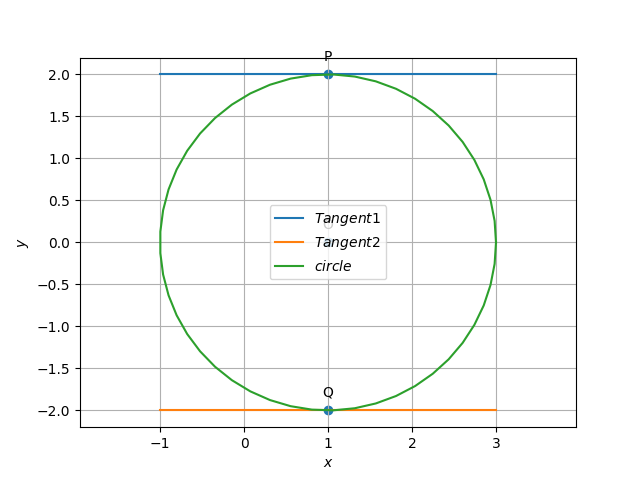
\includegraphics[width=\columnwidth]{./figs/circex/CircTangent.eps}
\caption{Tangents are parallel to the $x$-axis. }
\label{fig:CircTangent}	
\end{figure}

\end{enumerate}
}
\caption{}
\label{fig:8.5.16_circle_latex}	
\end{figure}
%
%
%\renewcommand{\thefigure}{\theenumi}
%
\item {\em Construction: }In Fig. \ref{fig:8.5.16_circle_latex} the known parameters are
%\label{}
\\
%
%\solution From the given information, 
%$\triangle ABC$ are 
\begin{align}
\vec{O} &= \myvec{0\\0} ,
\\
\vec{A} &= \myvec{r\\0} ,
\label{eq:8.5.16_constr_a}
\\
 \vec{B} &= \myvec{-r\\0} 
\label{eq:8.5.16_constr_b}
\\
\vec{C}&= r\myvec{\cos\theta\\\sin\theta}
\label{eq:8.5.16_constr_cgen}
\end{align}
%
Let 
\begin{align}
\vec{D} & = r\myvec{\cos\theta_1\\\sin\theta_1} 
\label{eq:8.5.16_constr_dgen}
\end{align}
From the given information,
\begin{align}
 \norm{\vec{D} - \vec{C}} &= r
\\
\implies \brak{\vec{D} - \vec{C}}^T\brak{\vec{D} - \vec{C}} &= r^2\\
 \label{eq:8.5.16_dist_formula}
\\
\implies  \norm{D} ^2 - 2\vec{D}^T\vec{C} +  \norm{C}^2 &=r^2 
\end{align}
In the above, 
\begin{align}
\because \norm{D} &= \norm{\vec{C}} = r,
\\
\frac{\vec{D}^T\vec{C}}{\norm{D}\norm{C}}  &= \frac{1}{2}
\\
\implies \cos \brak{\theta_1-\theta} &= 60 \degree
\label{eq:8.5.16_theta_diff}
\end{align}
using the definition of the inner product.  $\because \theta$ is known, we get $\theta_1$ from \eqref{eq:8.5.16_theta_diff}
and $\vec{D}$ from 
\eqref{eq:8.5.16_constr_dgen}. 
%
\subitem Thus,
\begin{align}
BD: \vec{x} &= \vec{B} + \lambda_1 \brak{\vec{B}-\vec{D}}
\\
AC: \vec{x} &= \vec{A} + \lambda_2 \brak{\vec{A}-\vec{C}}
\end{align}
%
which can be used to obtain $\vec{E}$.


%
General equation of conics is 
\begin{align}
    \vec{x}^T\vec{V}\vec{x}+ 2\vec{u}^T\vec{x}+f = 0
    \label{eq:solutions/1/16/eq:1}
\end{align}
Comparing with the equation given,
\begin{align}
\vec{V}=\myvec{\frac{1}{9} & 0 \\ 0 & \frac{1}{16}}\\
\vec{u}=\vec{0}\\
f=-1\\
\mydet{\vec{v}}=\mydet{\myvec{\frac{1}{9} & 0 \\ 0 & \frac{1}{16}}}>0
\end{align}
$\because \abs{\vec{V}}>0$, the given equation is of ellipse.\\
a)The tangents are parallel to the x-axis, hence, their direction and normal vectors, $\vec{m_1}$ and $\vec{n_1}$ are respectively,
\begin{align}
\vec{m_1}=\myvec{1\\0}\\
\vec{n_1}=\myvec{0\\1}
\end{align}
For an ellipse, given the normal vector $\vec{n}$, the tangent points of contact to the ellipse are given by
\begin{align}
    \vec{q}=\vec{V}^{-1}(\kappa \vec{n}-\vec{u})
    \label{eq:solutions/1/16/eq:2}
    =\vec{V}^{-1}\kappa \vec{n}
\end{align}
where
\begin{align}
    \kappa=\pm \sqrt{\frac{\vec{u^T}\vec{V}^{-1}\vec{u}-f}{\vec{n^T}\vec{V}^{-1}\vec{n}}}
    \label{eq:solutions/1/16/eq:2.0.9}\\
   =\pm \sqrt{\frac{-f}{\vec{n^T}\vec{V}^{-1}\vec{n}}}\\
    \vec{V}^{-1}=\myvec{9 & 0 \\ 0 & 16}\\
    \kappa_1=\pm \sqrt{\frac{-(-1)}{\myvec{0 & 1}\myvec{9 & 0 \\ 0 & 16} \myvec{0\\1}}}\\
 \implies \kappa_1=\pm \sqrt{\frac{1}{16}}\\
    \implies \kappa_1=\pm \frac{1}{4}      
\end{align}
From \eqref{eq:solutions/1/16/eq:2} , the point of contact $\vec{q_i}$ are,
\begin{align}
    \vec{q_1}=\myvec{9 & 0 \\ 0 & 16}\frac{1}{4}\myvec{0\\1}\\
    =\myvec{9 & 0 \\ 0 & 16}\myvec{0\\\frac{1}{4}}\\
    =\myvec{0\\4}\\
    \vec{q_2}=\myvec{9 & 0 \\ 0 & 16}\left(-\frac{1}{4}\right)\ \myvec{0\\1}\\
    =\myvec{9 & 0 \\ 0 & 16}\myvec{0\\-\frac{1}{4}}\\
    =\myvec{0\\-4}
\end{align}
b) The tangents are parallel to the y-axis, hence, their direction and normal vectors, $\vec{m_2}$ and $\vec{n_2}$ are respectively,
\begin{align}
\vec{m_2}=\myvec{0\\1}\\
\vec{n_2}=\myvec{1\\0}
\end{align}
Using equation \eqref{eq:solutions/1/16/eq:2.0.9}, the values of $\kappa$ for this case are
\begin{align}
     \kappa_2=\pm \sqrt{\frac{-(-1)}{\myvec{1 & 0}\myvec{9 & 0 \\ 0 & 16} \myvec{1\\0}}}\\
 \implies \kappa_2=\pm \sqrt{\frac{1}{9}}\\
    \implies \kappa_2=\pm \frac{1}{3} 
\end{align}
and from \eqref{eq:solutions/1/16/eq:2} , the point of contact $\vec{q_i}$ are,
\begin{align}
\vec{q_3}=\myvec{9 & 0 \\ 0 & 16}\frac{1}{3}\myvec{1\\0}\\
    =\myvec{9 & 0 \\ 0 & 16}\myvec{\frac{1}{3}\\0}\\
    =\myvec{3\\0}\\
\vec{q_4}=\myvec{9 & 0 \\ 0 & 16}\left(-\frac{1}{3}\right)\ \myvec{1\\0}\\
    =\myvec{9 & 0 \\ 0 & 16}\myvec{-\frac{1}{3}\\0}\\
    =\myvec{-3\\0}
\end{align}
 \begin{figure}[h!]
	\centering
	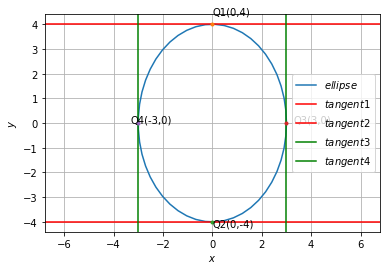
\includegraphics[width=\columnwidth]{./solutions/conics/1/16/ellipse.png}
	\caption{Figure depicting point of contact of tangents of ellipse parallel to x-axis and y-axis}
	\label{eq:solutions/1/16/fig1}
\end{figure}

%\end{enumerate}

\item $ABCE$ is a quadrilateral and $D$ is a point on $BC$ such that, $AC = AE, AB = AD$ and $\angle  BAD = \angle  EAC$. Show that $BC = DE$.
\\
\solution

General equation of conics is 
\begin{align}
    \vec{x}^T\vec{V}\vec{x}+ 2\vec{u}^T\vec{x}+f = 0
    \label{eq:solutions/1/16/eq:1}
\end{align}
Comparing with the equation given,
\begin{align}
\vec{V}=\myvec{\frac{1}{9} & 0 \\ 0 & \frac{1}{16}}\\
\vec{u}=\vec{0}\\
f=-1\\
\mydet{\vec{v}}=\mydet{\myvec{\frac{1}{9} & 0 \\ 0 & \frac{1}{16}}}>0
\end{align}
$\because \abs{\vec{V}}>0$, the given equation is of ellipse.\\
a)The tangents are parallel to the x-axis, hence, their direction and normal vectors, $\vec{m_1}$ and $\vec{n_1}$ are respectively,
\begin{align}
\vec{m_1}=\myvec{1\\0}\\
\vec{n_1}=\myvec{0\\1}
\end{align}
For an ellipse, given the normal vector $\vec{n}$, the tangent points of contact to the ellipse are given by
\begin{align}
    \vec{q}=\vec{V}^{-1}(\kappa \vec{n}-\vec{u})
    \label{eq:solutions/1/16/eq:2}
    =\vec{V}^{-1}\kappa \vec{n}
\end{align}
where
\begin{align}
    \kappa=\pm \sqrt{\frac{\vec{u^T}\vec{V}^{-1}\vec{u}-f}{\vec{n^T}\vec{V}^{-1}\vec{n}}}
    \label{eq:solutions/1/16/eq:2.0.9}\\
   =\pm \sqrt{\frac{-f}{\vec{n^T}\vec{V}^{-1}\vec{n}}}\\
    \vec{V}^{-1}=\myvec{9 & 0 \\ 0 & 16}\\
    \kappa_1=\pm \sqrt{\frac{-(-1)}{\myvec{0 & 1}\myvec{9 & 0 \\ 0 & 16} \myvec{0\\1}}}\\
 \implies \kappa_1=\pm \sqrt{\frac{1}{16}}\\
    \implies \kappa_1=\pm \frac{1}{4}      
\end{align}
From \eqref{eq:solutions/1/16/eq:2} , the point of contact $\vec{q_i}$ are,
\begin{align}
    \vec{q_1}=\myvec{9 & 0 \\ 0 & 16}\frac{1}{4}\myvec{0\\1}\\
    =\myvec{9 & 0 \\ 0 & 16}\myvec{0\\\frac{1}{4}}\\
    =\myvec{0\\4}\\
    \vec{q_2}=\myvec{9 & 0 \\ 0 & 16}\left(-\frac{1}{4}\right)\ \myvec{0\\1}\\
    =\myvec{9 & 0 \\ 0 & 16}\myvec{0\\-\frac{1}{4}}\\
    =\myvec{0\\-4}
\end{align}
b) The tangents are parallel to the y-axis, hence, their direction and normal vectors, $\vec{m_2}$ and $\vec{n_2}$ are respectively,
\begin{align}
\vec{m_2}=\myvec{0\\1}\\
\vec{n_2}=\myvec{1\\0}
\end{align}
Using equation \eqref{eq:solutions/1/16/eq:2.0.9}, the values of $\kappa$ for this case are
\begin{align}
     \kappa_2=\pm \sqrt{\frac{-(-1)}{\myvec{1 & 0}\myvec{9 & 0 \\ 0 & 16} \myvec{1\\0}}}\\
 \implies \kappa_2=\pm \sqrt{\frac{1}{9}}\\
    \implies \kappa_2=\pm \frac{1}{3} 
\end{align}
and from \eqref{eq:solutions/1/16/eq:2} , the point of contact $\vec{q_i}$ are,
\begin{align}
\vec{q_3}=\myvec{9 & 0 \\ 0 & 16}\frac{1}{3}\myvec{1\\0}\\
    =\myvec{9 & 0 \\ 0 & 16}\myvec{\frac{1}{3}\\0}\\
    =\myvec{3\\0}\\
\vec{q_4}=\myvec{9 & 0 \\ 0 & 16}\left(-\frac{1}{3}\right)\ \myvec{1\\0}\\
    =\myvec{9 & 0 \\ 0 & 16}\myvec{-\frac{1}{3}\\0}\\
    =\myvec{-3\\0}
\end{align}
 \begin{figure}[h!]
	\centering
	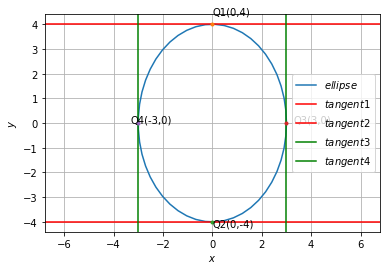
\includegraphics[width=\columnwidth]{./solutions/conics/1/16/ellipse.png}
	\caption{Figure depicting point of contact of tangents of ellipse parallel to x-axis and y-axis}
	\label{eq:solutions/1/16/fig1}
\end{figure}

%
\item In right triangle $ABC$, right angled at $C, M$ is the mid-point of hypotenuse $AB$. $C$ is joined to $M$ and produced to a point $D$ such that $DM = CM$. Point $D$ is joined to point $B$.
Show that: 
\begin{enumerate}
\item $ \triangle  AMC \cong  \triangle  BMD $
\item $\angle  DBC$ is a right angle. 
\item $\triangle  DBC \cong  \triangle  ACB$
\item $ CM = \frac{1}{ 2} AB$
\end{enumerate}
%
\solution

General equation of conics is 
\begin{align}
    \vec{x}^T\vec{V}\vec{x}+ 2\vec{u}^T\vec{x}+f = 0
    \label{eq:solutions/1/16/eq:1}
\end{align}
Comparing with the equation given,
\begin{align}
\vec{V}=\myvec{\frac{1}{9} & 0 \\ 0 & \frac{1}{16}}\\
\vec{u}=\vec{0}\\
f=-1\\
\mydet{\vec{v}}=\mydet{\myvec{\frac{1}{9} & 0 \\ 0 & \frac{1}{16}}}>0
\end{align}
$\because \abs{\vec{V}}>0$, the given equation is of ellipse.\\
a)The tangents are parallel to the x-axis, hence, their direction and normal vectors, $\vec{m_1}$ and $\vec{n_1}$ are respectively,
\begin{align}
\vec{m_1}=\myvec{1\\0}\\
\vec{n_1}=\myvec{0\\1}
\end{align}
For an ellipse, given the normal vector $\vec{n}$, the tangent points of contact to the ellipse are given by
\begin{align}
    \vec{q}=\vec{V}^{-1}(\kappa \vec{n}-\vec{u})
    \label{eq:solutions/1/16/eq:2}
    =\vec{V}^{-1}\kappa \vec{n}
\end{align}
where
\begin{align}
    \kappa=\pm \sqrt{\frac{\vec{u^T}\vec{V}^{-1}\vec{u}-f}{\vec{n^T}\vec{V}^{-1}\vec{n}}}
    \label{eq:solutions/1/16/eq:2.0.9}\\
   =\pm \sqrt{\frac{-f}{\vec{n^T}\vec{V}^{-1}\vec{n}}}\\
    \vec{V}^{-1}=\myvec{9 & 0 \\ 0 & 16}\\
    \kappa_1=\pm \sqrt{\frac{-(-1)}{\myvec{0 & 1}\myvec{9 & 0 \\ 0 & 16} \myvec{0\\1}}}\\
 \implies \kappa_1=\pm \sqrt{\frac{1}{16}}\\
    \implies \kappa_1=\pm \frac{1}{4}      
\end{align}
From \eqref{eq:solutions/1/16/eq:2} , the point of contact $\vec{q_i}$ are,
\begin{align}
    \vec{q_1}=\myvec{9 & 0 \\ 0 & 16}\frac{1}{4}\myvec{0\\1}\\
    =\myvec{9 & 0 \\ 0 & 16}\myvec{0\\\frac{1}{4}}\\
    =\myvec{0\\4}\\
    \vec{q_2}=\myvec{9 & 0 \\ 0 & 16}\left(-\frac{1}{4}\right)\ \myvec{0\\1}\\
    =\myvec{9 & 0 \\ 0 & 16}\myvec{0\\-\frac{1}{4}}\\
    =\myvec{0\\-4}
\end{align}
b) The tangents are parallel to the y-axis, hence, their direction and normal vectors, $\vec{m_2}$ and $\vec{n_2}$ are respectively,
\begin{align}
\vec{m_2}=\myvec{0\\1}\\
\vec{n_2}=\myvec{1\\0}
\end{align}
Using equation \eqref{eq:solutions/1/16/eq:2.0.9}, the values of $\kappa$ for this case are
\begin{align}
     \kappa_2=\pm \sqrt{\frac{-(-1)}{\myvec{1 & 0}\myvec{9 & 0 \\ 0 & 16} \myvec{1\\0}}}\\
 \implies \kappa_2=\pm \sqrt{\frac{1}{9}}\\
    \implies \kappa_2=\pm \frac{1}{3} 
\end{align}
and from \eqref{eq:solutions/1/16/eq:2} , the point of contact $\vec{q_i}$ are,
\begin{align}
\vec{q_3}=\myvec{9 & 0 \\ 0 & 16}\frac{1}{3}\myvec{1\\0}\\
    =\myvec{9 & 0 \\ 0 & 16}\myvec{\frac{1}{3}\\0}\\
    =\myvec{3\\0}\\
\vec{q_4}=\myvec{9 & 0 \\ 0 & 16}\left(-\frac{1}{3}\right)\ \myvec{1\\0}\\
    =\myvec{9 & 0 \\ 0 & 16}\myvec{-\frac{1}{3}\\0}\\
    =\myvec{-3\\0}
\end{align}
 \begin{figure}[h!]
	\centering
	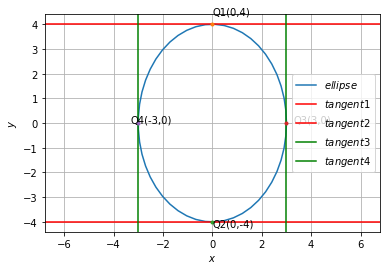
\includegraphics[width=\columnwidth]{./solutions/conics/1/16/ellipse.png}
	\caption{Figure depicting point of contact of tangents of ellipse parallel to x-axis and y-axis}
	\label{eq:solutions/1/16/fig1}
\end{figure}

%See  Fig. \ref{fig:8.1.28}.
%\solution 
%\begin{enumerate}
%
%\renewcommand{\thefigure}{\theenumi.\arabic{figure}}
\begin{figure}[!ht]
\centering
\resizebox{\columnwidth}{!}{\renewcommand{\theequation}{\theenumi}
\begin{enumerate}[label=\thesection.\arabic*.,ref=\thesection.\theenumi]
\numberwithin{equation}{enumi}
\item  Find the centre and radius of the circle 
\begin{align}
x^2+y^2+8x+10y-8 = 0
\label{eq:circ_basic}
\end{align}
\solution
\eqref{eq:circ_basic} can be expressed as 
\begin{align}
\vec{x}^T\vec{x}+ 2\myvec{4 & 5}\vec{x} -8 = 0
\end{align}
which is of the form \eqref{eq:conic_quad_form} with
\begin{align}
\label{eq:circ_basic_uf}
\vec{u} = \myvec{4\\5}, f = -8
\end{align}
From  Table \ref{table:conics}, the center and radius are given by 
\begin{align}
\vec{c} = -\vec{u} = \myvec{-4\\-5},
r = \sqrt{\norm{u}^2-f} = 7
\end{align}
\item Find the equation of a circle which passes through the points $\vec{P} = \myvec{2\\-2}$ and $\vec{Q} = \myvec{3\\4}$ and whose centre lies on the line  
%\cite{eleven}
\begin{align}
\label{eq:circ_ex1_line}
\myvec{1 & 1} \vec{x} = 2
\end{align}
\solution From \eqref{eq:conic_quad_form} and Table \ref{table:conics}, the equation of a circle can be expressed as
\begin{align}
\label{eq:circ_conic}
\vec{x}^T\vec{x}-2\vec{c}^T\vec{x}+f = 0
\end{align}
where $\vec{c}$ is the centre.
Substituting the given points in 
\eqref{eq:circ_conic} and using 
\eqref{eq:circ_ex1_line}, the following equations are obtained
\begin{align}
2\myvec{2 & -2}\vec{c} -  f &= 8
\\
2\myvec{3 & 4}\vec{c} -  f &= 25
\\
\myvec{1 & 1}\vec{c}  &= 2
\end{align}
which can be expressed as the matrix equation
\begin{align}
\myvec{
1 & 1 & 0
\\
4 & -4 & -1 
\\ 
6 & 8 & -1  
}
\myvec{\vec{c}\\f} = \myvec{2\\8\\25}
\end{align}
Row reducing the augmented matrix
\begin{align}
\myvec{
1 & 1 & 0 & 2
\\
4 & -4 & -1 & 8
\\ 
6 & 8 & -1  & 25
}
\\
\xleftrightarrow[R_3 \leftarrow R_3 -6R_1]{R_2 \leftarrow -R_2+4R_1}
\myvec{
1 & 1 & 0 & 2
\\
0 & 8 & 1 & 0
\\ 
0 & 2 & -1  & 13
}
\\
\xleftrightarrow[R_3 \leftarrow -\frac{4R_3 -R_2}{2}]{R_1 \leftarrow 8R_1-R_3}
\myvec{
8 & 0 & -1 & 16
\\
0 & 8 & 1 & 0
\\ 
0 & 0 & 5  & -52
}
\\
\xleftrightarrow[R_2 \leftarrow \frac{5R_2 -R_3}{4}]{R_1 \leftarrow \frac{5R_1+R_3}{4}}
\myvec{
10 & 0 & 0 & 7
\\
0 & 10 & 0 & 13
\\ 
0 & 0 & 5  & -52
}
\end{align}
Thus, 
\begin{align}
\vec{c} &= \frac{1}{10}\myvec{7\\13}
\\
f &=-\frac{52}{5}
\end{align}
which give the desired equation of the circle.
From Table \ref{table:conics},
%
\begin{align}
 r =  \sqrt{\norm{\vec{c}}^2-f} = \frac{1}{10}\sqrt{1258}
\end{align}
Fig. \ref{fig:CircOr}	verifies the above results.

\begin{figure}[!ht]
\centering
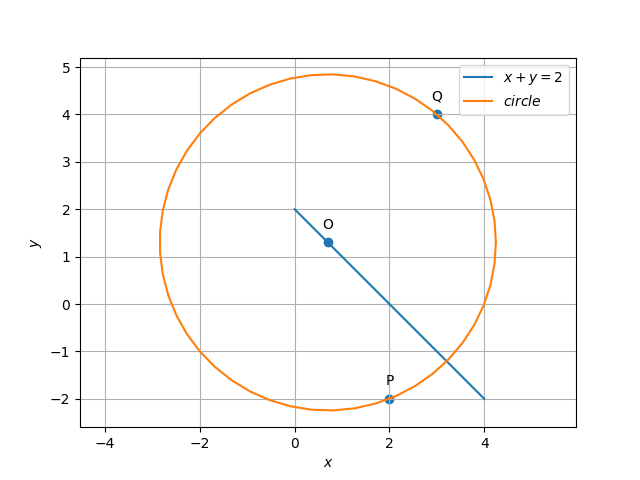
\includegraphics[width=\columnwidth]{./figs/circex/CircOr.eps}
\caption{Circle passing through $\myvec{2\\-2},\myvec{3\\4}$. Center is on line $\myvec{1 & 1}\vec{x}=2$. }
\label{fig:CircOr}	
\end{figure}

\item 
Find the points on the curve  
%\cite{twelve_one}
\begin{align}
x^2+y^2-2x-3 = 0
\label{eq:circle_tangent_prob}
\end{align}
at which the tangents are parallel to the $x$-axis.
\\
\solution \eqref{eq:circle_tangent_prob} can be expressed as
\begin{align}
\vec{x}^T\vec{x}+\myvec{-2 & 0}\vec{x}-3 &= 0
\label{eq:circle_tangent_prob_vec}
\\
\implies \vec{V} = \vec{I}, \vec{u} = \myvec{-1 \\ 0}, f = -3
\label{eq:circle_tangent_prob_uf}
\end{align}
From Table \ref{table:conics}, the centre and radius are
\begin{align}
\vec{c} = -\vec{u} = \myvec{-1 \\ 0}, r =\sqrt{\norm{\vec{u}}^2-f} = 2
\end{align}
$\because$ the tangents are parallel to the $x$-axis, their direction and normal vectors are respectively,
\begin{align}
\vec{m} = \myvec{1\\0},
\vec{n} = \myvec{0\\1}.
\end{align}
From Table \ref{table:conics},
\begin{align}
\kappa = \pm \sqrt{\frac{\vec{u}^T\vec{u}-f}{\vec{n}^T\vec{n}}} = \pm \sqrt{\frac{4}{1}} = \pm 2
\end{align}
and the desired points of contact are 
\begin{align}
\vec{q}_1, \vec{q}_2 = \myvec{1\\0}\pm 2\myvec{0\\1} =  
\myvec{1 \\  2},
\myvec{1 \\  -2}
\end{align}
%
Fig. \ref{fig:CircOr}	verifies the above results.
\begin{figure}[!ht]
\centering
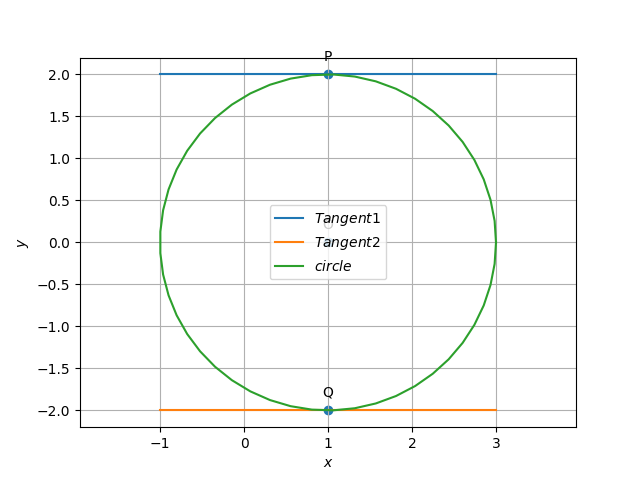
\includegraphics[width=\columnwidth]{./figs/circex/CircTangent.eps}
\caption{Tangents are parallel to the $x$-axis. }
\label{fig:CircTangent}	
\end{figure}

\end{enumerate}
}
\caption{}
\label{fig:8.5.16_circle_latex}	
\end{figure}
%
%
%\renewcommand{\thefigure}{\theenumi}
%
\item {\em Construction: }In Fig. \ref{fig:8.5.16_circle_latex} the known parameters are
%\label{}
\\
%
%\solution From the given information, 
%$\triangle ABC$ are 
\begin{align}
\vec{O} &= \myvec{0\\0} ,
\\
\vec{A} &= \myvec{r\\0} ,
\label{eq:8.5.16_constr_a}
\\
 \vec{B} &= \myvec{-r\\0} 
\label{eq:8.5.16_constr_b}
\\
\vec{C}&= r\myvec{\cos\theta\\\sin\theta}
\label{eq:8.5.16_constr_cgen}
\end{align}
%
Let 
\begin{align}
\vec{D} & = r\myvec{\cos\theta_1\\\sin\theta_1} 
\label{eq:8.5.16_constr_dgen}
\end{align}
From the given information,
\begin{align}
 \norm{\vec{D} - \vec{C}} &= r
\\
\implies \brak{\vec{D} - \vec{C}}^T\brak{\vec{D} - \vec{C}} &= r^2\\
 \label{eq:8.5.16_dist_formula}
\\
\implies  \norm{D} ^2 - 2\vec{D}^T\vec{C} +  \norm{C}^2 &=r^2 
\end{align}
In the above, 
\begin{align}
\because \norm{D} &= \norm{\vec{C}} = r,
\\
\frac{\vec{D}^T\vec{C}}{\norm{D}\norm{C}}  &= \frac{1}{2}
\\
\implies \cos \brak{\theta_1-\theta} &= 60 \degree
\label{eq:8.5.16_theta_diff}
\end{align}
using the definition of the inner product.  $\because \theta$ is known, we get $\theta_1$ from \eqref{eq:8.5.16_theta_diff}
and $\vec{D}$ from 
\eqref{eq:8.5.16_constr_dgen}. 
%
\subitem Thus,
\begin{align}
BD: \vec{x} &= \vec{B} + \lambda_1 \brak{\vec{B}-\vec{D}}
\\
AC: \vec{x} &= \vec{A} + \lambda_2 \brak{\vec{A}-\vec{C}}
\end{align}
%
which can be used to obtain $\vec{E}$.


%
General equation of conics is 
\begin{align}
    \vec{x}^T\vec{V}\vec{x}+ 2\vec{u}^T\vec{x}+f = 0
    \label{eq:solutions/1/16/eq:1}
\end{align}
Comparing with the equation given,
\begin{align}
\vec{V}=\myvec{\frac{1}{9} & 0 \\ 0 & \frac{1}{16}}\\
\vec{u}=\vec{0}\\
f=-1\\
\mydet{\vec{v}}=\mydet{\myvec{\frac{1}{9} & 0 \\ 0 & \frac{1}{16}}}>0
\end{align}
$\because \abs{\vec{V}}>0$, the given equation is of ellipse.\\
a)The tangents are parallel to the x-axis, hence, their direction and normal vectors, $\vec{m_1}$ and $\vec{n_1}$ are respectively,
\begin{align}
\vec{m_1}=\myvec{1\\0}\\
\vec{n_1}=\myvec{0\\1}
\end{align}
For an ellipse, given the normal vector $\vec{n}$, the tangent points of contact to the ellipse are given by
\begin{align}
    \vec{q}=\vec{V}^{-1}(\kappa \vec{n}-\vec{u})
    \label{eq:solutions/1/16/eq:2}
    =\vec{V}^{-1}\kappa \vec{n}
\end{align}
where
\begin{align}
    \kappa=\pm \sqrt{\frac{\vec{u^T}\vec{V}^{-1}\vec{u}-f}{\vec{n^T}\vec{V}^{-1}\vec{n}}}
    \label{eq:solutions/1/16/eq:2.0.9}\\
   =\pm \sqrt{\frac{-f}{\vec{n^T}\vec{V}^{-1}\vec{n}}}\\
    \vec{V}^{-1}=\myvec{9 & 0 \\ 0 & 16}\\
    \kappa_1=\pm \sqrt{\frac{-(-1)}{\myvec{0 & 1}\myvec{9 & 0 \\ 0 & 16} \myvec{0\\1}}}\\
 \implies \kappa_1=\pm \sqrt{\frac{1}{16}}\\
    \implies \kappa_1=\pm \frac{1}{4}      
\end{align}
From \eqref{eq:solutions/1/16/eq:2} , the point of contact $\vec{q_i}$ are,
\begin{align}
    \vec{q_1}=\myvec{9 & 0 \\ 0 & 16}\frac{1}{4}\myvec{0\\1}\\
    =\myvec{9 & 0 \\ 0 & 16}\myvec{0\\\frac{1}{4}}\\
    =\myvec{0\\4}\\
    \vec{q_2}=\myvec{9 & 0 \\ 0 & 16}\left(-\frac{1}{4}\right)\ \myvec{0\\1}\\
    =\myvec{9 & 0 \\ 0 & 16}\myvec{0\\-\frac{1}{4}}\\
    =\myvec{0\\-4}
\end{align}
b) The tangents are parallel to the y-axis, hence, their direction and normal vectors, $\vec{m_2}$ and $\vec{n_2}$ are respectively,
\begin{align}
\vec{m_2}=\myvec{0\\1}\\
\vec{n_2}=\myvec{1\\0}
\end{align}
Using equation \eqref{eq:solutions/1/16/eq:2.0.9}, the values of $\kappa$ for this case are
\begin{align}
     \kappa_2=\pm \sqrt{\frac{-(-1)}{\myvec{1 & 0}\myvec{9 & 0 \\ 0 & 16} \myvec{1\\0}}}\\
 \implies \kappa_2=\pm \sqrt{\frac{1}{9}}\\
    \implies \kappa_2=\pm \frac{1}{3} 
\end{align}
and from \eqref{eq:solutions/1/16/eq:2} , the point of contact $\vec{q_i}$ are,
\begin{align}
\vec{q_3}=\myvec{9 & 0 \\ 0 & 16}\frac{1}{3}\myvec{1\\0}\\
    =\myvec{9 & 0 \\ 0 & 16}\myvec{\frac{1}{3}\\0}\\
    =\myvec{3\\0}\\
\vec{q_4}=\myvec{9 & 0 \\ 0 & 16}\left(-\frac{1}{3}\right)\ \myvec{1\\0}\\
    =\myvec{9 & 0 \\ 0 & 16}\myvec{-\frac{1}{3}\\0}\\
    =\myvec{-3\\0}
\end{align}
 \begin{figure}[h!]
	\centering
	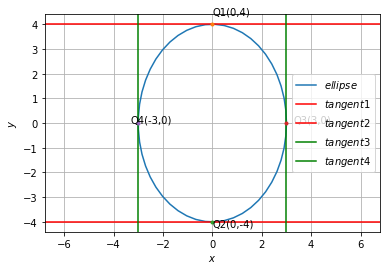
\includegraphics[width=\columnwidth]{./solutions/conics/1/16/ellipse.png}
	\caption{Figure depicting point of contact of tangents of ellipse parallel to x-axis and y-axis}
	\label{eq:solutions/1/16/fig1}
\end{figure}

%\end{enumerate}

\item In an isosceles $\triangle ABC$, with $AB = AC$, the bisectors of $\angle B$ and $\angle C$ intersect each other at $O$. Join $A$ to $O$. Show that :
\begin{enumerate} 
\item $OB = OC$ 
\item $AO$ bisects $\angle A$
\end{enumerate}
\item In $\triangle ABC$, $AD$ is the perpendicular bisector of $BC$. Show that $\triangle ABC$ is an isosceles triangle in which $AB = AC$.
\\
\solution 

General equation of conics is 
\begin{align}
    \vec{x}^T\vec{V}\vec{x}+ 2\vec{u}^T\vec{x}+f = 0
    \label{eq:solutions/1/16/eq:1}
\end{align}
Comparing with the equation given,
\begin{align}
\vec{V}=\myvec{\frac{1}{9} & 0 \\ 0 & \frac{1}{16}}\\
\vec{u}=\vec{0}\\
f=-1\\
\mydet{\vec{v}}=\mydet{\myvec{\frac{1}{9} & 0 \\ 0 & \frac{1}{16}}}>0
\end{align}
$\because \abs{\vec{V}}>0$, the given equation is of ellipse.\\
a)The tangents are parallel to the x-axis, hence, their direction and normal vectors, $\vec{m_1}$ and $\vec{n_1}$ are respectively,
\begin{align}
\vec{m_1}=\myvec{1\\0}\\
\vec{n_1}=\myvec{0\\1}
\end{align}
For an ellipse, given the normal vector $\vec{n}$, the tangent points of contact to the ellipse are given by
\begin{align}
    \vec{q}=\vec{V}^{-1}(\kappa \vec{n}-\vec{u})
    \label{eq:solutions/1/16/eq:2}
    =\vec{V}^{-1}\kappa \vec{n}
\end{align}
where
\begin{align}
    \kappa=\pm \sqrt{\frac{\vec{u^T}\vec{V}^{-1}\vec{u}-f}{\vec{n^T}\vec{V}^{-1}\vec{n}}}
    \label{eq:solutions/1/16/eq:2.0.9}\\
   =\pm \sqrt{\frac{-f}{\vec{n^T}\vec{V}^{-1}\vec{n}}}\\
    \vec{V}^{-1}=\myvec{9 & 0 \\ 0 & 16}\\
    \kappa_1=\pm \sqrt{\frac{-(-1)}{\myvec{0 & 1}\myvec{9 & 0 \\ 0 & 16} \myvec{0\\1}}}\\
 \implies \kappa_1=\pm \sqrt{\frac{1}{16}}\\
    \implies \kappa_1=\pm \frac{1}{4}      
\end{align}
From \eqref{eq:solutions/1/16/eq:2} , the point of contact $\vec{q_i}$ are,
\begin{align}
    \vec{q_1}=\myvec{9 & 0 \\ 0 & 16}\frac{1}{4}\myvec{0\\1}\\
    =\myvec{9 & 0 \\ 0 & 16}\myvec{0\\\frac{1}{4}}\\
    =\myvec{0\\4}\\
    \vec{q_2}=\myvec{9 & 0 \\ 0 & 16}\left(-\frac{1}{4}\right)\ \myvec{0\\1}\\
    =\myvec{9 & 0 \\ 0 & 16}\myvec{0\\-\frac{1}{4}}\\
    =\myvec{0\\-4}
\end{align}
b) The tangents are parallel to the y-axis, hence, their direction and normal vectors, $\vec{m_2}$ and $\vec{n_2}$ are respectively,
\begin{align}
\vec{m_2}=\myvec{0\\1}\\
\vec{n_2}=\myvec{1\\0}
\end{align}
Using equation \eqref{eq:solutions/1/16/eq:2.0.9}, the values of $\kappa$ for this case are
\begin{align}
     \kappa_2=\pm \sqrt{\frac{-(-1)}{\myvec{1 & 0}\myvec{9 & 0 \\ 0 & 16} \myvec{1\\0}}}\\
 \implies \kappa_2=\pm \sqrt{\frac{1}{9}}\\
    \implies \kappa_2=\pm \frac{1}{3} 
\end{align}
and from \eqref{eq:solutions/1/16/eq:2} , the point of contact $\vec{q_i}$ are,
\begin{align}
\vec{q_3}=\myvec{9 & 0 \\ 0 & 16}\frac{1}{3}\myvec{1\\0}\\
    =\myvec{9 & 0 \\ 0 & 16}\myvec{\frac{1}{3}\\0}\\
    =\myvec{3\\0}\\
\vec{q_4}=\myvec{9 & 0 \\ 0 & 16}\left(-\frac{1}{3}\right)\ \myvec{1\\0}\\
    =\myvec{9 & 0 \\ 0 & 16}\myvec{-\frac{1}{3}\\0}\\
    =\myvec{-3\\0}
\end{align}
 \begin{figure}[h!]
	\centering
	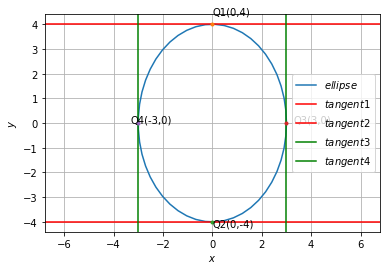
\includegraphics[width=\columnwidth]{./solutions/conics/1/16/ellipse.png}
	\caption{Figure depicting point of contact of tangents of ellipse parallel to x-axis and y-axis}
	\label{eq:solutions/1/16/fig1}
\end{figure}


\item $ABC$ is an isosceles triangle in which altitudes $BE$ and $CF$ are drawn to equal sides $AC$ and $AB$ respectively . Show that these altitudes are equal.
%
\\
\solution

General equation of conics is 
\begin{align}
    \vec{x}^T\vec{V}\vec{x}+ 2\vec{u}^T\vec{x}+f = 0
    \label{eq:solutions/1/16/eq:1}
\end{align}
Comparing with the equation given,
\begin{align}
\vec{V}=\myvec{\frac{1}{9} & 0 \\ 0 & \frac{1}{16}}\\
\vec{u}=\vec{0}\\
f=-1\\
\mydet{\vec{v}}=\mydet{\myvec{\frac{1}{9} & 0 \\ 0 & \frac{1}{16}}}>0
\end{align}
$\because \abs{\vec{V}}>0$, the given equation is of ellipse.\\
a)The tangents are parallel to the x-axis, hence, their direction and normal vectors, $\vec{m_1}$ and $\vec{n_1}$ are respectively,
\begin{align}
\vec{m_1}=\myvec{1\\0}\\
\vec{n_1}=\myvec{0\\1}
\end{align}
For an ellipse, given the normal vector $\vec{n}$, the tangent points of contact to the ellipse are given by
\begin{align}
    \vec{q}=\vec{V}^{-1}(\kappa \vec{n}-\vec{u})
    \label{eq:solutions/1/16/eq:2}
    =\vec{V}^{-1}\kappa \vec{n}
\end{align}
where
\begin{align}
    \kappa=\pm \sqrt{\frac{\vec{u^T}\vec{V}^{-1}\vec{u}-f}{\vec{n^T}\vec{V}^{-1}\vec{n}}}
    \label{eq:solutions/1/16/eq:2.0.9}\\
   =\pm \sqrt{\frac{-f}{\vec{n^T}\vec{V}^{-1}\vec{n}}}\\
    \vec{V}^{-1}=\myvec{9 & 0 \\ 0 & 16}\\
    \kappa_1=\pm \sqrt{\frac{-(-1)}{\myvec{0 & 1}\myvec{9 & 0 \\ 0 & 16} \myvec{0\\1}}}\\
 \implies \kappa_1=\pm \sqrt{\frac{1}{16}}\\
    \implies \kappa_1=\pm \frac{1}{4}      
\end{align}
From \eqref{eq:solutions/1/16/eq:2} , the point of contact $\vec{q_i}$ are,
\begin{align}
    \vec{q_1}=\myvec{9 & 0 \\ 0 & 16}\frac{1}{4}\myvec{0\\1}\\
    =\myvec{9 & 0 \\ 0 & 16}\myvec{0\\\frac{1}{4}}\\
    =\myvec{0\\4}\\
    \vec{q_2}=\myvec{9 & 0 \\ 0 & 16}\left(-\frac{1}{4}\right)\ \myvec{0\\1}\\
    =\myvec{9 & 0 \\ 0 & 16}\myvec{0\\-\frac{1}{4}}\\
    =\myvec{0\\-4}
\end{align}
b) The tangents are parallel to the y-axis, hence, their direction and normal vectors, $\vec{m_2}$ and $\vec{n_2}$ are respectively,
\begin{align}
\vec{m_2}=\myvec{0\\1}\\
\vec{n_2}=\myvec{1\\0}
\end{align}
Using equation \eqref{eq:solutions/1/16/eq:2.0.9}, the values of $\kappa$ for this case are
\begin{align}
     \kappa_2=\pm \sqrt{\frac{-(-1)}{\myvec{1 & 0}\myvec{9 & 0 \\ 0 & 16} \myvec{1\\0}}}\\
 \implies \kappa_2=\pm \sqrt{\frac{1}{9}}\\
    \implies \kappa_2=\pm \frac{1}{3} 
\end{align}
and from \eqref{eq:solutions/1/16/eq:2} , the point of contact $\vec{q_i}$ are,
\begin{align}
\vec{q_3}=\myvec{9 & 0 \\ 0 & 16}\frac{1}{3}\myvec{1\\0}\\
    =\myvec{9 & 0 \\ 0 & 16}\myvec{\frac{1}{3}\\0}\\
    =\myvec{3\\0}\\
\vec{q_4}=\myvec{9 & 0 \\ 0 & 16}\left(-\frac{1}{3}\right)\ \myvec{1\\0}\\
    =\myvec{9 & 0 \\ 0 & 16}\myvec{-\frac{1}{3}\\0}\\
    =\myvec{-3\\0}
\end{align}
 \begin{figure}[h!]
	\centering
	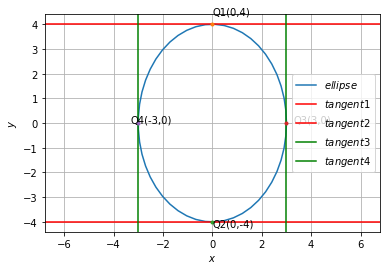
\includegraphics[width=\columnwidth]{./solutions/conics/1/16/ellipse.png}
	\caption{Figure depicting point of contact of tangents of ellipse parallel to x-axis and y-axis}
	\label{eq:solutions/1/16/fig1}
\end{figure}


\item $ABC$ is a triangle in which altitudes $BE$ and $CF$ to sides $AC$ and $AB$ are equal. Show that
%
\begin{enumerate} 
\item $\triangle  ABE \cong  \triangle  ACF $
\item  $AB = AC$, i.e., $ABC$ is an isosceles triangle.
\end{enumerate}
%
\solution

General equation of conics is 
\begin{align}
    \vec{x}^T\vec{V}\vec{x}+ 2\vec{u}^T\vec{x}+f = 0
    \label{eq:solutions/1/16/eq:1}
\end{align}
Comparing with the equation given,
\begin{align}
\vec{V}=\myvec{\frac{1}{9} & 0 \\ 0 & \frac{1}{16}}\\
\vec{u}=\vec{0}\\
f=-1\\
\mydet{\vec{v}}=\mydet{\myvec{\frac{1}{9} & 0 \\ 0 & \frac{1}{16}}}>0
\end{align}
$\because \abs{\vec{V}}>0$, the given equation is of ellipse.\\
a)The tangents are parallel to the x-axis, hence, their direction and normal vectors, $\vec{m_1}$ and $\vec{n_1}$ are respectively,
\begin{align}
\vec{m_1}=\myvec{1\\0}\\
\vec{n_1}=\myvec{0\\1}
\end{align}
For an ellipse, given the normal vector $\vec{n}$, the tangent points of contact to the ellipse are given by
\begin{align}
    \vec{q}=\vec{V}^{-1}(\kappa \vec{n}-\vec{u})
    \label{eq:solutions/1/16/eq:2}
    =\vec{V}^{-1}\kappa \vec{n}
\end{align}
where
\begin{align}
    \kappa=\pm \sqrt{\frac{\vec{u^T}\vec{V}^{-1}\vec{u}-f}{\vec{n^T}\vec{V}^{-1}\vec{n}}}
    \label{eq:solutions/1/16/eq:2.0.9}\\
   =\pm \sqrt{\frac{-f}{\vec{n^T}\vec{V}^{-1}\vec{n}}}\\
    \vec{V}^{-1}=\myvec{9 & 0 \\ 0 & 16}\\
    \kappa_1=\pm \sqrt{\frac{-(-1)}{\myvec{0 & 1}\myvec{9 & 0 \\ 0 & 16} \myvec{0\\1}}}\\
 \implies \kappa_1=\pm \sqrt{\frac{1}{16}}\\
    \implies \kappa_1=\pm \frac{1}{4}      
\end{align}
From \eqref{eq:solutions/1/16/eq:2} , the point of contact $\vec{q_i}$ are,
\begin{align}
    \vec{q_1}=\myvec{9 & 0 \\ 0 & 16}\frac{1}{4}\myvec{0\\1}\\
    =\myvec{9 & 0 \\ 0 & 16}\myvec{0\\\frac{1}{4}}\\
    =\myvec{0\\4}\\
    \vec{q_2}=\myvec{9 & 0 \\ 0 & 16}\left(-\frac{1}{4}\right)\ \myvec{0\\1}\\
    =\myvec{9 & 0 \\ 0 & 16}\myvec{0\\-\frac{1}{4}}\\
    =\myvec{0\\-4}
\end{align}
b) The tangents are parallel to the y-axis, hence, their direction and normal vectors, $\vec{m_2}$ and $\vec{n_2}$ are respectively,
\begin{align}
\vec{m_2}=\myvec{0\\1}\\
\vec{n_2}=\myvec{1\\0}
\end{align}
Using equation \eqref{eq:solutions/1/16/eq:2.0.9}, the values of $\kappa$ for this case are
\begin{align}
     \kappa_2=\pm \sqrt{\frac{-(-1)}{\myvec{1 & 0}\myvec{9 & 0 \\ 0 & 16} \myvec{1\\0}}}\\
 \implies \kappa_2=\pm \sqrt{\frac{1}{9}}\\
    \implies \kappa_2=\pm \frac{1}{3} 
\end{align}
and from \eqref{eq:solutions/1/16/eq:2} , the point of contact $\vec{q_i}$ are,
\begin{align}
\vec{q_3}=\myvec{9 & 0 \\ 0 & 16}\frac{1}{3}\myvec{1\\0}\\
    =\myvec{9 & 0 \\ 0 & 16}\myvec{\frac{1}{3}\\0}\\
    =\myvec{3\\0}\\
\vec{q_4}=\myvec{9 & 0 \\ 0 & 16}\left(-\frac{1}{3}\right)\ \myvec{1\\0}\\
    =\myvec{9 & 0 \\ 0 & 16}\myvec{-\frac{1}{3}\\0}\\
    =\myvec{-3\\0}
\end{align}
 \begin{figure}[h!]
	\centering
	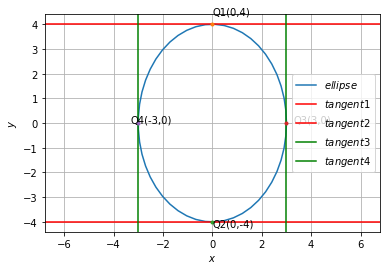
\includegraphics[width=\columnwidth]{./solutions/conics/1/16/ellipse.png}
	\caption{Figure depicting point of contact of tangents of ellipse parallel to x-axis and y-axis}
	\label{eq:solutions/1/16/fig1}
\end{figure}


\item $ABC$ and $DBC$ are two isosceles triangles on the same base $BC$. Show that $\angle ABD = \angle ACD$.
%
\solution

General equation of conics is 
\begin{align}
    \vec{x}^T\vec{V}\vec{x}+ 2\vec{u}^T\vec{x}+f = 0
    \label{eq:solutions/1/16/eq:1}
\end{align}
Comparing with the equation given,
\begin{align}
\vec{V}=\myvec{\frac{1}{9} & 0 \\ 0 & \frac{1}{16}}\\
\vec{u}=\vec{0}\\
f=-1\\
\mydet{\vec{v}}=\mydet{\myvec{\frac{1}{9} & 0 \\ 0 & \frac{1}{16}}}>0
\end{align}
$\because \abs{\vec{V}}>0$, the given equation is of ellipse.\\
a)The tangents are parallel to the x-axis, hence, their direction and normal vectors, $\vec{m_1}$ and $\vec{n_1}$ are respectively,
\begin{align}
\vec{m_1}=\myvec{1\\0}\\
\vec{n_1}=\myvec{0\\1}
\end{align}
For an ellipse, given the normal vector $\vec{n}$, the tangent points of contact to the ellipse are given by
\begin{align}
    \vec{q}=\vec{V}^{-1}(\kappa \vec{n}-\vec{u})
    \label{eq:solutions/1/16/eq:2}
    =\vec{V}^{-1}\kappa \vec{n}
\end{align}
where
\begin{align}
    \kappa=\pm \sqrt{\frac{\vec{u^T}\vec{V}^{-1}\vec{u}-f}{\vec{n^T}\vec{V}^{-1}\vec{n}}}
    \label{eq:solutions/1/16/eq:2.0.9}\\
   =\pm \sqrt{\frac{-f}{\vec{n^T}\vec{V}^{-1}\vec{n}}}\\
    \vec{V}^{-1}=\myvec{9 & 0 \\ 0 & 16}\\
    \kappa_1=\pm \sqrt{\frac{-(-1)}{\myvec{0 & 1}\myvec{9 & 0 \\ 0 & 16} \myvec{0\\1}}}\\
 \implies \kappa_1=\pm \sqrt{\frac{1}{16}}\\
    \implies \kappa_1=\pm \frac{1}{4}      
\end{align}
From \eqref{eq:solutions/1/16/eq:2} , the point of contact $\vec{q_i}$ are,
\begin{align}
    \vec{q_1}=\myvec{9 & 0 \\ 0 & 16}\frac{1}{4}\myvec{0\\1}\\
    =\myvec{9 & 0 \\ 0 & 16}\myvec{0\\\frac{1}{4}}\\
    =\myvec{0\\4}\\
    \vec{q_2}=\myvec{9 & 0 \\ 0 & 16}\left(-\frac{1}{4}\right)\ \myvec{0\\1}\\
    =\myvec{9 & 0 \\ 0 & 16}\myvec{0\\-\frac{1}{4}}\\
    =\myvec{0\\-4}
\end{align}
b) The tangents are parallel to the y-axis, hence, their direction and normal vectors, $\vec{m_2}$ and $\vec{n_2}$ are respectively,
\begin{align}
\vec{m_2}=\myvec{0\\1}\\
\vec{n_2}=\myvec{1\\0}
\end{align}
Using equation \eqref{eq:solutions/1/16/eq:2.0.9}, the values of $\kappa$ for this case are
\begin{align}
     \kappa_2=\pm \sqrt{\frac{-(-1)}{\myvec{1 & 0}\myvec{9 & 0 \\ 0 & 16} \myvec{1\\0}}}\\
 \implies \kappa_2=\pm \sqrt{\frac{1}{9}}\\
    \implies \kappa_2=\pm \frac{1}{3} 
\end{align}
and from \eqref{eq:solutions/1/16/eq:2} , the point of contact $\vec{q_i}$ are,
\begin{align}
\vec{q_3}=\myvec{9 & 0 \\ 0 & 16}\frac{1}{3}\myvec{1\\0}\\
    =\myvec{9 & 0 \\ 0 & 16}\myvec{\frac{1}{3}\\0}\\
    =\myvec{3\\0}\\
\vec{q_4}=\myvec{9 & 0 \\ 0 & 16}\left(-\frac{1}{3}\right)\ \myvec{1\\0}\\
    =\myvec{9 & 0 \\ 0 & 16}\myvec{-\frac{1}{3}\\0}\\
    =\myvec{-3\\0}
\end{align}
 \begin{figure}[h!]
	\centering
	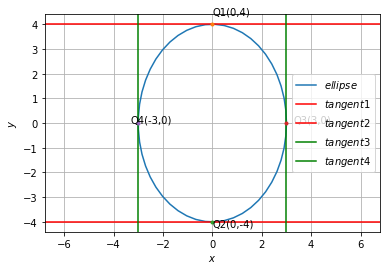
\includegraphics[width=\columnwidth]{./solutions/conics/1/16/ellipse.png}
	\caption{Figure depicting point of contact of tangents of ellipse parallel to x-axis and y-axis}
	\label{eq:solutions/1/16/fig1}
\end{figure}

\item  $\triangle  ABC$ and $\triangle  DBC$ are two isosceles triangles on the same base $BC$ and vertices $A$ and $D$ are on the same side of $BC$. If $AD$ is extended to intersect $BC$ at $P$, show that
\begin{enumerate}
\item $\triangle  ABD \cong  \triangle  ACD $
\item $\triangle  ABP \cong  \triangle  ACP $
\item $AP$ bisects $\angle  A$ as well as $\angle  D$. 
\item $AP$ is the perpendicular bisector of $BC$.
\end{enumerate}
\solution

General equation of conics is 
\begin{align}
    \vec{x}^T\vec{V}\vec{x}+ 2\vec{u}^T\vec{x}+f = 0
    \label{eq:solutions/1/16/eq:1}
\end{align}
Comparing with the equation given,
\begin{align}
\vec{V}=\myvec{\frac{1}{9} & 0 \\ 0 & \frac{1}{16}}\\
\vec{u}=\vec{0}\\
f=-1\\
\mydet{\vec{v}}=\mydet{\myvec{\frac{1}{9} & 0 \\ 0 & \frac{1}{16}}}>0
\end{align}
$\because \abs{\vec{V}}>0$, the given equation is of ellipse.\\
a)The tangents are parallel to the x-axis, hence, their direction and normal vectors, $\vec{m_1}$ and $\vec{n_1}$ are respectively,
\begin{align}
\vec{m_1}=\myvec{1\\0}\\
\vec{n_1}=\myvec{0\\1}
\end{align}
For an ellipse, given the normal vector $\vec{n}$, the tangent points of contact to the ellipse are given by
\begin{align}
    \vec{q}=\vec{V}^{-1}(\kappa \vec{n}-\vec{u})
    \label{eq:solutions/1/16/eq:2}
    =\vec{V}^{-1}\kappa \vec{n}
\end{align}
where
\begin{align}
    \kappa=\pm \sqrt{\frac{\vec{u^T}\vec{V}^{-1}\vec{u}-f}{\vec{n^T}\vec{V}^{-1}\vec{n}}}
    \label{eq:solutions/1/16/eq:2.0.9}\\
   =\pm \sqrt{\frac{-f}{\vec{n^T}\vec{V}^{-1}\vec{n}}}\\
    \vec{V}^{-1}=\myvec{9 & 0 \\ 0 & 16}\\
    \kappa_1=\pm \sqrt{\frac{-(-1)}{\myvec{0 & 1}\myvec{9 & 0 \\ 0 & 16} \myvec{0\\1}}}\\
 \implies \kappa_1=\pm \sqrt{\frac{1}{16}}\\
    \implies \kappa_1=\pm \frac{1}{4}      
\end{align}
From \eqref{eq:solutions/1/16/eq:2} , the point of contact $\vec{q_i}$ are,
\begin{align}
    \vec{q_1}=\myvec{9 & 0 \\ 0 & 16}\frac{1}{4}\myvec{0\\1}\\
    =\myvec{9 & 0 \\ 0 & 16}\myvec{0\\\frac{1}{4}}\\
    =\myvec{0\\4}\\
    \vec{q_2}=\myvec{9 & 0 \\ 0 & 16}\left(-\frac{1}{4}\right)\ \myvec{0\\1}\\
    =\myvec{9 & 0 \\ 0 & 16}\myvec{0\\-\frac{1}{4}}\\
    =\myvec{0\\-4}
\end{align}
b) The tangents are parallel to the y-axis, hence, their direction and normal vectors, $\vec{m_2}$ and $\vec{n_2}$ are respectively,
\begin{align}
\vec{m_2}=\myvec{0\\1}\\
\vec{n_2}=\myvec{1\\0}
\end{align}
Using equation \eqref{eq:solutions/1/16/eq:2.0.9}, the values of $\kappa$ for this case are
\begin{align}
     \kappa_2=\pm \sqrt{\frac{-(-1)}{\myvec{1 & 0}\myvec{9 & 0 \\ 0 & 16} \myvec{1\\0}}}\\
 \implies \kappa_2=\pm \sqrt{\frac{1}{9}}\\
    \implies \kappa_2=\pm \frac{1}{3} 
\end{align}
and from \eqref{eq:solutions/1/16/eq:2} , the point of contact $\vec{q_i}$ are,
\begin{align}
\vec{q_3}=\myvec{9 & 0 \\ 0 & 16}\frac{1}{3}\myvec{1\\0}\\
    =\myvec{9 & 0 \\ 0 & 16}\myvec{\frac{1}{3}\\0}\\
    =\myvec{3\\0}\\
\vec{q_4}=\myvec{9 & 0 \\ 0 & 16}\left(-\frac{1}{3}\right)\ \myvec{1\\0}\\
    =\myvec{9 & 0 \\ 0 & 16}\myvec{-\frac{1}{3}\\0}\\
    =\myvec{-3\\0}
\end{align}
 \begin{figure}[h!]
	\centering
	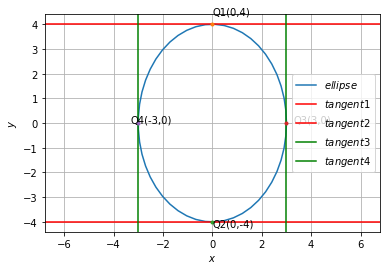
\includegraphics[width=\columnwidth]{./solutions/conics/1/16/ellipse.png}
	\caption{Figure depicting point of contact of tangents of ellipse parallel to x-axis and y-axis}
	\label{eq:solutions/1/16/fig1}
\end{figure}

\item $AD$ is an altitude of an isosceles $\triangle ABC$ in which $AB = AC$. Show that 
\begin{enumerate}
\item $AD$ bisects $BC$
\item $AD$ bisects $\angle  A$. 
\end{enumerate}
\solution

General equation of conics is 
\begin{align}
    \vec{x}^T\vec{V}\vec{x}+ 2\vec{u}^T\vec{x}+f = 0
    \label{eq:solutions/1/16/eq:1}
\end{align}
Comparing with the equation given,
\begin{align}
\vec{V}=\myvec{\frac{1}{9} & 0 \\ 0 & \frac{1}{16}}\\
\vec{u}=\vec{0}\\
f=-1\\
\mydet{\vec{v}}=\mydet{\myvec{\frac{1}{9} & 0 \\ 0 & \frac{1}{16}}}>0
\end{align}
$\because \abs{\vec{V}}>0$, the given equation is of ellipse.\\
a)The tangents are parallel to the x-axis, hence, their direction and normal vectors, $\vec{m_1}$ and $\vec{n_1}$ are respectively,
\begin{align}
\vec{m_1}=\myvec{1\\0}\\
\vec{n_1}=\myvec{0\\1}
\end{align}
For an ellipse, given the normal vector $\vec{n}$, the tangent points of contact to the ellipse are given by
\begin{align}
    \vec{q}=\vec{V}^{-1}(\kappa \vec{n}-\vec{u})
    \label{eq:solutions/1/16/eq:2}
    =\vec{V}^{-1}\kappa \vec{n}
\end{align}
where
\begin{align}
    \kappa=\pm \sqrt{\frac{\vec{u^T}\vec{V}^{-1}\vec{u}-f}{\vec{n^T}\vec{V}^{-1}\vec{n}}}
    \label{eq:solutions/1/16/eq:2.0.9}\\
   =\pm \sqrt{\frac{-f}{\vec{n^T}\vec{V}^{-1}\vec{n}}}\\
    \vec{V}^{-1}=\myvec{9 & 0 \\ 0 & 16}\\
    \kappa_1=\pm \sqrt{\frac{-(-1)}{\myvec{0 & 1}\myvec{9 & 0 \\ 0 & 16} \myvec{0\\1}}}\\
 \implies \kappa_1=\pm \sqrt{\frac{1}{16}}\\
    \implies \kappa_1=\pm \frac{1}{4}      
\end{align}
From \eqref{eq:solutions/1/16/eq:2} , the point of contact $\vec{q_i}$ are,
\begin{align}
    \vec{q_1}=\myvec{9 & 0 \\ 0 & 16}\frac{1}{4}\myvec{0\\1}\\
    =\myvec{9 & 0 \\ 0 & 16}\myvec{0\\\frac{1}{4}}\\
    =\myvec{0\\4}\\
    \vec{q_2}=\myvec{9 & 0 \\ 0 & 16}\left(-\frac{1}{4}\right)\ \myvec{0\\1}\\
    =\myvec{9 & 0 \\ 0 & 16}\myvec{0\\-\frac{1}{4}}\\
    =\myvec{0\\-4}
\end{align}
b) The tangents are parallel to the y-axis, hence, their direction and normal vectors, $\vec{m_2}$ and $\vec{n_2}$ are respectively,
\begin{align}
\vec{m_2}=\myvec{0\\1}\\
\vec{n_2}=\myvec{1\\0}
\end{align}
Using equation \eqref{eq:solutions/1/16/eq:2.0.9}, the values of $\kappa$ for this case are
\begin{align}
     \kappa_2=\pm \sqrt{\frac{-(-1)}{\myvec{1 & 0}\myvec{9 & 0 \\ 0 & 16} \myvec{1\\0}}}\\
 \implies \kappa_2=\pm \sqrt{\frac{1}{9}}\\
    \implies \kappa_2=\pm \frac{1}{3} 
\end{align}
and from \eqref{eq:solutions/1/16/eq:2} , the point of contact $\vec{q_i}$ are,
\begin{align}
\vec{q_3}=\myvec{9 & 0 \\ 0 & 16}\frac{1}{3}\myvec{1\\0}\\
    =\myvec{9 & 0 \\ 0 & 16}\myvec{\frac{1}{3}\\0}\\
    =\myvec{3\\0}\\
\vec{q_4}=\myvec{9 & 0 \\ 0 & 16}\left(-\frac{1}{3}\right)\ \myvec{1\\0}\\
    =\myvec{9 & 0 \\ 0 & 16}\myvec{-\frac{1}{3}\\0}\\
    =\myvec{-3\\0}
\end{align}
 \begin{figure}[h!]
	\centering
	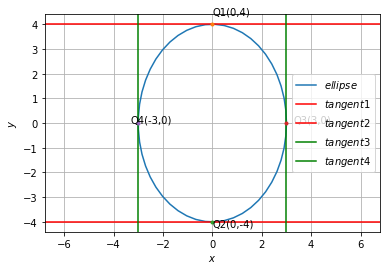
\includegraphics[width=\columnwidth]{./solutions/conics/1/16/ellipse.png}
	\caption{Figure depicting point of contact of tangents of ellipse parallel to x-axis and y-axis}
	\label{eq:solutions/1/16/fig1}
\end{figure}


\item  Two sides $AB$ and $BC$ and median $AM$ of one triangle $ABC$ are respectively equal to sides $PQ$ and $QR$ and median $PN$ of $\triangle  PQR$. Show that: 
\begin{enumerate}
\item $\triangle  ABM \cong  \triangle  PQN $
\item $\triangle  ABC \cong  \triangle  PQR$
\end{enumerate}
\solution

General equation of conics is 
\begin{align}
    \vec{x}^T\vec{V}\vec{x}+ 2\vec{u}^T\vec{x}+f = 0
    \label{eq:solutions/1/16/eq:1}
\end{align}
Comparing with the equation given,
\begin{align}
\vec{V}=\myvec{\frac{1}{9} & 0 \\ 0 & \frac{1}{16}}\\
\vec{u}=\vec{0}\\
f=-1\\
\mydet{\vec{v}}=\mydet{\myvec{\frac{1}{9} & 0 \\ 0 & \frac{1}{16}}}>0
\end{align}
$\because \abs{\vec{V}}>0$, the given equation is of ellipse.\\
a)The tangents are parallel to the x-axis, hence, their direction and normal vectors, $\vec{m_1}$ and $\vec{n_1}$ are respectively,
\begin{align}
\vec{m_1}=\myvec{1\\0}\\
\vec{n_1}=\myvec{0\\1}
\end{align}
For an ellipse, given the normal vector $\vec{n}$, the tangent points of contact to the ellipse are given by
\begin{align}
    \vec{q}=\vec{V}^{-1}(\kappa \vec{n}-\vec{u})
    \label{eq:solutions/1/16/eq:2}
    =\vec{V}^{-1}\kappa \vec{n}
\end{align}
where
\begin{align}
    \kappa=\pm \sqrt{\frac{\vec{u^T}\vec{V}^{-1}\vec{u}-f}{\vec{n^T}\vec{V}^{-1}\vec{n}}}
    \label{eq:solutions/1/16/eq:2.0.9}\\
   =\pm \sqrt{\frac{-f}{\vec{n^T}\vec{V}^{-1}\vec{n}}}\\
    \vec{V}^{-1}=\myvec{9 & 0 \\ 0 & 16}\\
    \kappa_1=\pm \sqrt{\frac{-(-1)}{\myvec{0 & 1}\myvec{9 & 0 \\ 0 & 16} \myvec{0\\1}}}\\
 \implies \kappa_1=\pm \sqrt{\frac{1}{16}}\\
    \implies \kappa_1=\pm \frac{1}{4}      
\end{align}
From \eqref{eq:solutions/1/16/eq:2} , the point of contact $\vec{q_i}$ are,
\begin{align}
    \vec{q_1}=\myvec{9 & 0 \\ 0 & 16}\frac{1}{4}\myvec{0\\1}\\
    =\myvec{9 & 0 \\ 0 & 16}\myvec{0\\\frac{1}{4}}\\
    =\myvec{0\\4}\\
    \vec{q_2}=\myvec{9 & 0 \\ 0 & 16}\left(-\frac{1}{4}\right)\ \myvec{0\\1}\\
    =\myvec{9 & 0 \\ 0 & 16}\myvec{0\\-\frac{1}{4}}\\
    =\myvec{0\\-4}
\end{align}
b) The tangents are parallel to the y-axis, hence, their direction and normal vectors, $\vec{m_2}$ and $\vec{n_2}$ are respectively,
\begin{align}
\vec{m_2}=\myvec{0\\1}\\
\vec{n_2}=\myvec{1\\0}
\end{align}
Using equation \eqref{eq:solutions/1/16/eq:2.0.9}, the values of $\kappa$ for this case are
\begin{align}
     \kappa_2=\pm \sqrt{\frac{-(-1)}{\myvec{1 & 0}\myvec{9 & 0 \\ 0 & 16} \myvec{1\\0}}}\\
 \implies \kappa_2=\pm \sqrt{\frac{1}{9}}\\
    \implies \kappa_2=\pm \frac{1}{3} 
\end{align}
and from \eqref{eq:solutions/1/16/eq:2} , the point of contact $\vec{q_i}$ are,
\begin{align}
\vec{q_3}=\myvec{9 & 0 \\ 0 & 16}\frac{1}{3}\myvec{1\\0}\\
    =\myvec{9 & 0 \\ 0 & 16}\myvec{\frac{1}{3}\\0}\\
    =\myvec{3\\0}\\
\vec{q_4}=\myvec{9 & 0 \\ 0 & 16}\left(-\frac{1}{3}\right)\ \myvec{1\\0}\\
    =\myvec{9 & 0 \\ 0 & 16}\myvec{-\frac{1}{3}\\0}\\
    =\myvec{-3\\0}
\end{align}
 \begin{figure}[h!]
	\centering
	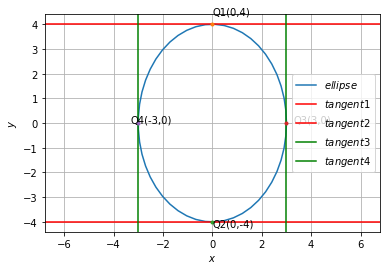
\includegraphics[width=\columnwidth]{./solutions/conics/1/16/ellipse.png}
	\caption{Figure depicting point of contact of tangents of ellipse parallel to x-axis and y-axis}
	\label{eq:solutions/1/16/fig1}
\end{figure}


%\begin{enumerate}
%
%\renewcommand{\thefigure}{\theenumi.\arabic{figure}}
\begin{figure}[!ht]
\centering
\resizebox{\columnwidth}{!}{\renewcommand{\theequation}{\theenumi}
\begin{enumerate}[label=\thesection.\arabic*.,ref=\thesection.\theenumi]
\numberwithin{equation}{enumi}
\item  Find the centre and radius of the circle 
\begin{align}
x^2+y^2+8x+10y-8 = 0
\label{eq:circ_basic}
\end{align}
\solution
\eqref{eq:circ_basic} can be expressed as 
\begin{align}
\vec{x}^T\vec{x}+ 2\myvec{4 & 5}\vec{x} -8 = 0
\end{align}
which is of the form \eqref{eq:conic_quad_form} with
\begin{align}
\label{eq:circ_basic_uf}
\vec{u} = \myvec{4\\5}, f = -8
\end{align}
From  Table \ref{table:conics}, the center and radius are given by 
\begin{align}
\vec{c} = -\vec{u} = \myvec{-4\\-5},
r = \sqrt{\norm{u}^2-f} = 7
\end{align}
\item Find the equation of a circle which passes through the points $\vec{P} = \myvec{2\\-2}$ and $\vec{Q} = \myvec{3\\4}$ and whose centre lies on the line  
%\cite{eleven}
\begin{align}
\label{eq:circ_ex1_line}
\myvec{1 & 1} \vec{x} = 2
\end{align}
\solution From \eqref{eq:conic_quad_form} and Table \ref{table:conics}, the equation of a circle can be expressed as
\begin{align}
\label{eq:circ_conic}
\vec{x}^T\vec{x}-2\vec{c}^T\vec{x}+f = 0
\end{align}
where $\vec{c}$ is the centre.
Substituting the given points in 
\eqref{eq:circ_conic} and using 
\eqref{eq:circ_ex1_line}, the following equations are obtained
\begin{align}
2\myvec{2 & -2}\vec{c} -  f &= 8
\\
2\myvec{3 & 4}\vec{c} -  f &= 25
\\
\myvec{1 & 1}\vec{c}  &= 2
\end{align}
which can be expressed as the matrix equation
\begin{align}
\myvec{
1 & 1 & 0
\\
4 & -4 & -1 
\\ 
6 & 8 & -1  
}
\myvec{\vec{c}\\f} = \myvec{2\\8\\25}
\end{align}
Row reducing the augmented matrix
\begin{align}
\myvec{
1 & 1 & 0 & 2
\\
4 & -4 & -1 & 8
\\ 
6 & 8 & -1  & 25
}
\\
\xleftrightarrow[R_3 \leftarrow R_3 -6R_1]{R_2 \leftarrow -R_2+4R_1}
\myvec{
1 & 1 & 0 & 2
\\
0 & 8 & 1 & 0
\\ 
0 & 2 & -1  & 13
}
\\
\xleftrightarrow[R_3 \leftarrow -\frac{4R_3 -R_2}{2}]{R_1 \leftarrow 8R_1-R_3}
\myvec{
8 & 0 & -1 & 16
\\
0 & 8 & 1 & 0
\\ 
0 & 0 & 5  & -52
}
\\
\xleftrightarrow[R_2 \leftarrow \frac{5R_2 -R_3}{4}]{R_1 \leftarrow \frac{5R_1+R_3}{4}}
\myvec{
10 & 0 & 0 & 7
\\
0 & 10 & 0 & 13
\\ 
0 & 0 & 5  & -52
}
\end{align}
Thus, 
\begin{align}
\vec{c} &= \frac{1}{10}\myvec{7\\13}
\\
f &=-\frac{52}{5}
\end{align}
which give the desired equation of the circle.
From Table \ref{table:conics},
%
\begin{align}
 r =  \sqrt{\norm{\vec{c}}^2-f} = \frac{1}{10}\sqrt{1258}
\end{align}
Fig. \ref{fig:CircOr}	verifies the above results.

\begin{figure}[!ht]
\centering
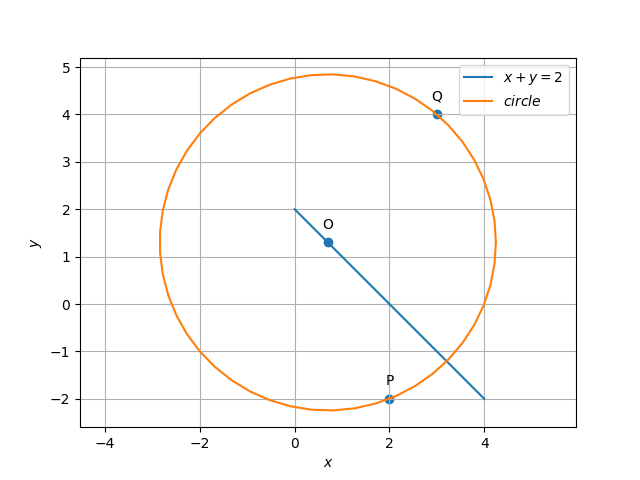
\includegraphics[width=\columnwidth]{./figs/circex/CircOr.eps}
\caption{Circle passing through $\myvec{2\\-2},\myvec{3\\4}$. Center is on line $\myvec{1 & 1}\vec{x}=2$. }
\label{fig:CircOr}	
\end{figure}

\item 
Find the points on the curve  
%\cite{twelve_one}
\begin{align}
x^2+y^2-2x-3 = 0
\label{eq:circle_tangent_prob}
\end{align}
at which the tangents are parallel to the $x$-axis.
\\
\solution \eqref{eq:circle_tangent_prob} can be expressed as
\begin{align}
\vec{x}^T\vec{x}+\myvec{-2 & 0}\vec{x}-3 &= 0
\label{eq:circle_tangent_prob_vec}
\\
\implies \vec{V} = \vec{I}, \vec{u} = \myvec{-1 \\ 0}, f = -3
\label{eq:circle_tangent_prob_uf}
\end{align}
From Table \ref{table:conics}, the centre and radius are
\begin{align}
\vec{c} = -\vec{u} = \myvec{-1 \\ 0}, r =\sqrt{\norm{\vec{u}}^2-f} = 2
\end{align}
$\because$ the tangents are parallel to the $x$-axis, their direction and normal vectors are respectively,
\begin{align}
\vec{m} = \myvec{1\\0},
\vec{n} = \myvec{0\\1}.
\end{align}
From Table \ref{table:conics},
\begin{align}
\kappa = \pm \sqrt{\frac{\vec{u}^T\vec{u}-f}{\vec{n}^T\vec{n}}} = \pm \sqrt{\frac{4}{1}} = \pm 2
\end{align}
and the desired points of contact are 
\begin{align}
\vec{q}_1, \vec{q}_2 = \myvec{1\\0}\pm 2\myvec{0\\1} =  
\myvec{1 \\  2},
\myvec{1 \\  -2}
\end{align}
%
Fig. \ref{fig:CircOr}	verifies the above results.
\begin{figure}[!ht]
\centering
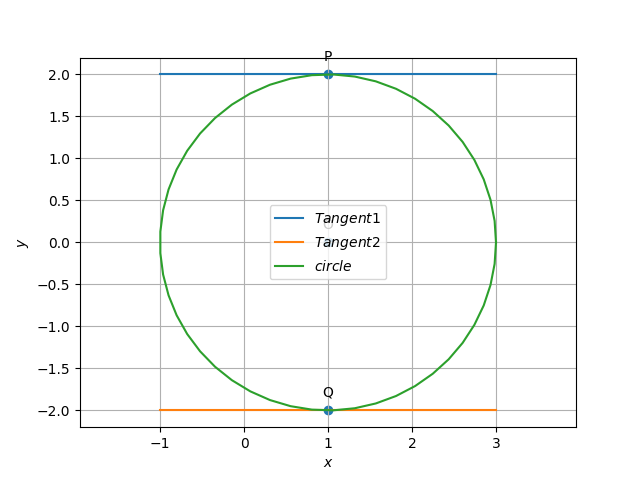
\includegraphics[width=\columnwidth]{./figs/circex/CircTangent.eps}
\caption{Tangents are parallel to the $x$-axis. }
\label{fig:CircTangent}	
\end{figure}

\end{enumerate}
}
\caption{}
\label{fig:8.5.16_circle_latex}	
\end{figure}
%
%
%\renewcommand{\thefigure}{\theenumi}
%
\item {\em Construction: }In Fig. \ref{fig:8.5.16_circle_latex} the known parameters are
%\label{}
\\
%
%\solution From the given information, 
%$\triangle ABC$ are 
\begin{align}
\vec{O} &= \myvec{0\\0} ,
\\
\vec{A} &= \myvec{r\\0} ,
\label{eq:8.5.16_constr_a}
\\
 \vec{B} &= \myvec{-r\\0} 
\label{eq:8.5.16_constr_b}
\\
\vec{C}&= r\myvec{\cos\theta\\\sin\theta}
\label{eq:8.5.16_constr_cgen}
\end{align}
%
Let 
\begin{align}
\vec{D} & = r\myvec{\cos\theta_1\\\sin\theta_1} 
\label{eq:8.5.16_constr_dgen}
\end{align}
From the given information,
\begin{align}
 \norm{\vec{D} - \vec{C}} &= r
\\
\implies \brak{\vec{D} - \vec{C}}^T\brak{\vec{D} - \vec{C}} &= r^2\\
 \label{eq:8.5.16_dist_formula}
\\
\implies  \norm{D} ^2 - 2\vec{D}^T\vec{C} +  \norm{C}^2 &=r^2 
\end{align}
In the above, 
\begin{align}
\because \norm{D} &= \norm{\vec{C}} = r,
\\
\frac{\vec{D}^T\vec{C}}{\norm{D}\norm{C}}  &= \frac{1}{2}
\\
\implies \cos \brak{\theta_1-\theta} &= 60 \degree
\label{eq:8.5.16_theta_diff}
\end{align}
using the definition of the inner product.  $\because \theta$ is known, we get $\theta_1$ from \eqref{eq:8.5.16_theta_diff}
and $\vec{D}$ from 
\eqref{eq:8.5.16_constr_dgen}. 
%
\subitem Thus,
\begin{align}
BD: \vec{x} &= \vec{B} + \lambda_1 \brak{\vec{B}-\vec{D}}
\\
AC: \vec{x} &= \vec{A} + \lambda_2 \brak{\vec{A}-\vec{C}}
\end{align}
%
which can be used to obtain $\vec{E}$.


%%
General equation of conics is 
\begin{align}
    \vec{x}^T\vec{V}\vec{x}+ 2\vec{u}^T\vec{x}+f = 0
    \label{eq:solutions/1/16/eq:1}
\end{align}
Comparing with the equation given,
\begin{align}
\vec{V}=\myvec{\frac{1}{9} & 0 \\ 0 & \frac{1}{16}}\\
\vec{u}=\vec{0}\\
f=-1\\
\mydet{\vec{v}}=\mydet{\myvec{\frac{1}{9} & 0 \\ 0 & \frac{1}{16}}}>0
\end{align}
$\because \abs{\vec{V}}>0$, the given equation is of ellipse.\\
a)The tangents are parallel to the x-axis, hence, their direction and normal vectors, $\vec{m_1}$ and $\vec{n_1}$ are respectively,
\begin{align}
\vec{m_1}=\myvec{1\\0}\\
\vec{n_1}=\myvec{0\\1}
\end{align}
For an ellipse, given the normal vector $\vec{n}$, the tangent points of contact to the ellipse are given by
\begin{align}
    \vec{q}=\vec{V}^{-1}(\kappa \vec{n}-\vec{u})
    \label{eq:solutions/1/16/eq:2}
    =\vec{V}^{-1}\kappa \vec{n}
\end{align}
where
\begin{align}
    \kappa=\pm \sqrt{\frac{\vec{u^T}\vec{V}^{-1}\vec{u}-f}{\vec{n^T}\vec{V}^{-1}\vec{n}}}
    \label{eq:solutions/1/16/eq:2.0.9}\\
   =\pm \sqrt{\frac{-f}{\vec{n^T}\vec{V}^{-1}\vec{n}}}\\
    \vec{V}^{-1}=\myvec{9 & 0 \\ 0 & 16}\\
    \kappa_1=\pm \sqrt{\frac{-(-1)}{\myvec{0 & 1}\myvec{9 & 0 \\ 0 & 16} \myvec{0\\1}}}\\
 \implies \kappa_1=\pm \sqrt{\frac{1}{16}}\\
    \implies \kappa_1=\pm \frac{1}{4}      
\end{align}
From \eqref{eq:solutions/1/16/eq:2} , the point of contact $\vec{q_i}$ are,
\begin{align}
    \vec{q_1}=\myvec{9 & 0 \\ 0 & 16}\frac{1}{4}\myvec{0\\1}\\
    =\myvec{9 & 0 \\ 0 & 16}\myvec{0\\\frac{1}{4}}\\
    =\myvec{0\\4}\\
    \vec{q_2}=\myvec{9 & 0 \\ 0 & 16}\left(-\frac{1}{4}\right)\ \myvec{0\\1}\\
    =\myvec{9 & 0 \\ 0 & 16}\myvec{0\\-\frac{1}{4}}\\
    =\myvec{0\\-4}
\end{align}
b) The tangents are parallel to the y-axis, hence, their direction and normal vectors, $\vec{m_2}$ and $\vec{n_2}$ are respectively,
\begin{align}
\vec{m_2}=\myvec{0\\1}\\
\vec{n_2}=\myvec{1\\0}
\end{align}
Using equation \eqref{eq:solutions/1/16/eq:2.0.9}, the values of $\kappa$ for this case are
\begin{align}
     \kappa_2=\pm \sqrt{\frac{-(-1)}{\myvec{1 & 0}\myvec{9 & 0 \\ 0 & 16} \myvec{1\\0}}}\\
 \implies \kappa_2=\pm \sqrt{\frac{1}{9}}\\
    \implies \kappa_2=\pm \frac{1}{3} 
\end{align}
and from \eqref{eq:solutions/1/16/eq:2} , the point of contact $\vec{q_i}$ are,
\begin{align}
\vec{q_3}=\myvec{9 & 0 \\ 0 & 16}\frac{1}{3}\myvec{1\\0}\\
    =\myvec{9 & 0 \\ 0 & 16}\myvec{\frac{1}{3}\\0}\\
    =\myvec{3\\0}\\
\vec{q_4}=\myvec{9 & 0 \\ 0 & 16}\left(-\frac{1}{3}\right)\ \myvec{1\\0}\\
    =\myvec{9 & 0 \\ 0 & 16}\myvec{-\frac{1}{3}\\0}\\
    =\myvec{-3\\0}
\end{align}
 \begin{figure}[h!]
	\centering
	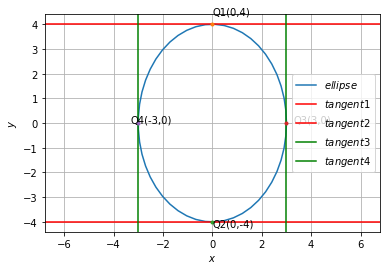
\includegraphics[width=\columnwidth]{./solutions/conics/1/16/ellipse.png}
	\caption{Figure depicting point of contact of tangents of ellipse parallel to x-axis and y-axis}
	\label{eq:solutions/1/16/fig1}
\end{figure}

%\end{enumerate}

\item  $BE$ and $CF$ are two equal altitudes of a triangle $ABC$. Using RHS congruence rule, prove that the triangle $ABC$ is isosceles.
\solution

General equation of conics is 
\begin{align}
    \vec{x}^T\vec{V}\vec{x}+ 2\vec{u}^T\vec{x}+f = 0
    \label{eq:solutions/1/16/eq:1}
\end{align}
Comparing with the equation given,
\begin{align}
\vec{V}=\myvec{\frac{1}{9} & 0 \\ 0 & \frac{1}{16}}\\
\vec{u}=\vec{0}\\
f=-1\\
\mydet{\vec{v}}=\mydet{\myvec{\frac{1}{9} & 0 \\ 0 & \frac{1}{16}}}>0
\end{align}
$\because \abs{\vec{V}}>0$, the given equation is of ellipse.\\
a)The tangents are parallel to the x-axis, hence, their direction and normal vectors, $\vec{m_1}$ and $\vec{n_1}$ are respectively,
\begin{align}
\vec{m_1}=\myvec{1\\0}\\
\vec{n_1}=\myvec{0\\1}
\end{align}
For an ellipse, given the normal vector $\vec{n}$, the tangent points of contact to the ellipse are given by
\begin{align}
    \vec{q}=\vec{V}^{-1}(\kappa \vec{n}-\vec{u})
    \label{eq:solutions/1/16/eq:2}
    =\vec{V}^{-1}\kappa \vec{n}
\end{align}
where
\begin{align}
    \kappa=\pm \sqrt{\frac{\vec{u^T}\vec{V}^{-1}\vec{u}-f}{\vec{n^T}\vec{V}^{-1}\vec{n}}}
    \label{eq:solutions/1/16/eq:2.0.9}\\
   =\pm \sqrt{\frac{-f}{\vec{n^T}\vec{V}^{-1}\vec{n}}}\\
    \vec{V}^{-1}=\myvec{9 & 0 \\ 0 & 16}\\
    \kappa_1=\pm \sqrt{\frac{-(-1)}{\myvec{0 & 1}\myvec{9 & 0 \\ 0 & 16} \myvec{0\\1}}}\\
 \implies \kappa_1=\pm \sqrt{\frac{1}{16}}\\
    \implies \kappa_1=\pm \frac{1}{4}      
\end{align}
From \eqref{eq:solutions/1/16/eq:2} , the point of contact $\vec{q_i}$ are,
\begin{align}
    \vec{q_1}=\myvec{9 & 0 \\ 0 & 16}\frac{1}{4}\myvec{0\\1}\\
    =\myvec{9 & 0 \\ 0 & 16}\myvec{0\\\frac{1}{4}}\\
    =\myvec{0\\4}\\
    \vec{q_2}=\myvec{9 & 0 \\ 0 & 16}\left(-\frac{1}{4}\right)\ \myvec{0\\1}\\
    =\myvec{9 & 0 \\ 0 & 16}\myvec{0\\-\frac{1}{4}}\\
    =\myvec{0\\-4}
\end{align}
b) The tangents are parallel to the y-axis, hence, their direction and normal vectors, $\vec{m_2}$ and $\vec{n_2}$ are respectively,
\begin{align}
\vec{m_2}=\myvec{0\\1}\\
\vec{n_2}=\myvec{1\\0}
\end{align}
Using equation \eqref{eq:solutions/1/16/eq:2.0.9}, the values of $\kappa$ for this case are
\begin{align}
     \kappa_2=\pm \sqrt{\frac{-(-1)}{\myvec{1 & 0}\myvec{9 & 0 \\ 0 & 16} \myvec{1\\0}}}\\
 \implies \kappa_2=\pm \sqrt{\frac{1}{9}}\\
    \implies \kappa_2=\pm \frac{1}{3} 
\end{align}
and from \eqref{eq:solutions/1/16/eq:2} , the point of contact $\vec{q_i}$ are,
\begin{align}
\vec{q_3}=\myvec{9 & 0 \\ 0 & 16}\frac{1}{3}\myvec{1\\0}\\
    =\myvec{9 & 0 \\ 0 & 16}\myvec{\frac{1}{3}\\0}\\
    =\myvec{3\\0}\\
\vec{q_4}=\myvec{9 & 0 \\ 0 & 16}\left(-\frac{1}{3}\right)\ \myvec{1\\0}\\
    =\myvec{9 & 0 \\ 0 & 16}\myvec{-\frac{1}{3}\\0}\\
    =\myvec{-3\\0}
\end{align}
 \begin{figure}[h!]
	\centering
	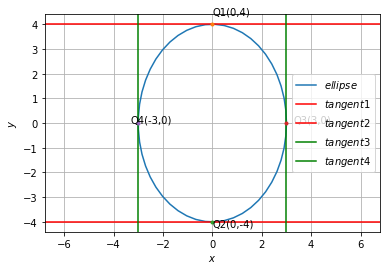
\includegraphics[width=\columnwidth]{./solutions/conics/1/16/ellipse.png}
	\caption{Figure depicting point of contact of tangents of ellipse parallel to x-axis and y-axis}
	\label{eq:solutions/1/16/fig1}
\end{figure}

\item  $ABC$ is an isosceles triangle with $AB = AC$. Draw $AP \perp BC$ to show that $\angle  B = \angle  C$.
%
\item $\triangle ABC$ is an isosceles triangle in which $AB = AC$. Side $BA$ is produced to $D$ such that $AD = AB$. Show that $\angle BCD$ is a right angle.
%
\solution

General equation of conics is 
\begin{align}
    \vec{x}^T\vec{V}\vec{x}+ 2\vec{u}^T\vec{x}+f = 0
    \label{eq:solutions/1/16/eq:1}
\end{align}
Comparing with the equation given,
\begin{align}
\vec{V}=\myvec{\frac{1}{9} & 0 \\ 0 & \frac{1}{16}}\\
\vec{u}=\vec{0}\\
f=-1\\
\mydet{\vec{v}}=\mydet{\myvec{\frac{1}{9} & 0 \\ 0 & \frac{1}{16}}}>0
\end{align}
$\because \abs{\vec{V}}>0$, the given equation is of ellipse.\\
a)The tangents are parallel to the x-axis, hence, their direction and normal vectors, $\vec{m_1}$ and $\vec{n_1}$ are respectively,
\begin{align}
\vec{m_1}=\myvec{1\\0}\\
\vec{n_1}=\myvec{0\\1}
\end{align}
For an ellipse, given the normal vector $\vec{n}$, the tangent points of contact to the ellipse are given by
\begin{align}
    \vec{q}=\vec{V}^{-1}(\kappa \vec{n}-\vec{u})
    \label{eq:solutions/1/16/eq:2}
    =\vec{V}^{-1}\kappa \vec{n}
\end{align}
where
\begin{align}
    \kappa=\pm \sqrt{\frac{\vec{u^T}\vec{V}^{-1}\vec{u}-f}{\vec{n^T}\vec{V}^{-1}\vec{n}}}
    \label{eq:solutions/1/16/eq:2.0.9}\\
   =\pm \sqrt{\frac{-f}{\vec{n^T}\vec{V}^{-1}\vec{n}}}\\
    \vec{V}^{-1}=\myvec{9 & 0 \\ 0 & 16}\\
    \kappa_1=\pm \sqrt{\frac{-(-1)}{\myvec{0 & 1}\myvec{9 & 0 \\ 0 & 16} \myvec{0\\1}}}\\
 \implies \kappa_1=\pm \sqrt{\frac{1}{16}}\\
    \implies \kappa_1=\pm \frac{1}{4}      
\end{align}
From \eqref{eq:solutions/1/16/eq:2} , the point of contact $\vec{q_i}$ are,
\begin{align}
    \vec{q_1}=\myvec{9 & 0 \\ 0 & 16}\frac{1}{4}\myvec{0\\1}\\
    =\myvec{9 & 0 \\ 0 & 16}\myvec{0\\\frac{1}{4}}\\
    =\myvec{0\\4}\\
    \vec{q_2}=\myvec{9 & 0 \\ 0 & 16}\left(-\frac{1}{4}\right)\ \myvec{0\\1}\\
    =\myvec{9 & 0 \\ 0 & 16}\myvec{0\\-\frac{1}{4}}\\
    =\myvec{0\\-4}
\end{align}
b) The tangents are parallel to the y-axis, hence, their direction and normal vectors, $\vec{m_2}$ and $\vec{n_2}$ are respectively,
\begin{align}
\vec{m_2}=\myvec{0\\1}\\
\vec{n_2}=\myvec{1\\0}
\end{align}
Using equation \eqref{eq:solutions/1/16/eq:2.0.9}, the values of $\kappa$ for this case are
\begin{align}
     \kappa_2=\pm \sqrt{\frac{-(-1)}{\myvec{1 & 0}\myvec{9 & 0 \\ 0 & 16} \myvec{1\\0}}}\\
 \implies \kappa_2=\pm \sqrt{\frac{1}{9}}\\
    \implies \kappa_2=\pm \frac{1}{3} 
\end{align}
and from \eqref{eq:solutions/1/16/eq:2} , the point of contact $\vec{q_i}$ are,
\begin{align}
\vec{q_3}=\myvec{9 & 0 \\ 0 & 16}\frac{1}{3}\myvec{1\\0}\\
    =\myvec{9 & 0 \\ 0 & 16}\myvec{\frac{1}{3}\\0}\\
    =\myvec{3\\0}\\
\vec{q_4}=\myvec{9 & 0 \\ 0 & 16}\left(-\frac{1}{3}\right)\ \myvec{1\\0}\\
    =\myvec{9 & 0 \\ 0 & 16}\myvec{-\frac{1}{3}\\0}\\
    =\myvec{-3\\0}
\end{align}
 \begin{figure}[h!]
	\centering
	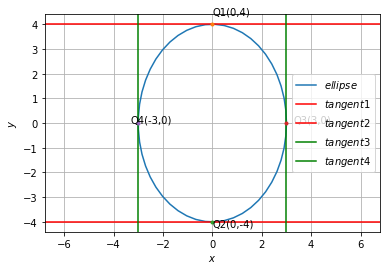
\includegraphics[width=\columnwidth]{./solutions/conics/1/16/ellipse.png}
	\caption{Figure depicting point of contact of tangents of ellipse parallel to x-axis and y-axis}
	\label{eq:solutions/1/16/fig1}
\end{figure}

\item $ABC$ is a right angled triangle in which $\angle A$ = 90$\degree$ and $AB = AC$. Find $\angle B$ and $\angle C$.
%
\item Show that in a right angled triangle, the hypotenuse is the longest side.
\item Sides AB and AC of $\triangle  ABC$ are extended to points P and Q respectively. Also, $\angle  PBC < \angle  QCB$. Show that $AC > AB$.
\solution

General equation of conics is 
\begin{align}
    \vec{x}^T\vec{V}\vec{x}+ 2\vec{u}^T\vec{x}+f = 0
    \label{eq:solutions/1/16/eq:1}
\end{align}
Comparing with the equation given,
\begin{align}
\vec{V}=\myvec{\frac{1}{9} & 0 \\ 0 & \frac{1}{16}}\\
\vec{u}=\vec{0}\\
f=-1\\
\mydet{\vec{v}}=\mydet{\myvec{\frac{1}{9} & 0 \\ 0 & \frac{1}{16}}}>0
\end{align}
$\because \abs{\vec{V}}>0$, the given equation is of ellipse.\\
a)The tangents are parallel to the x-axis, hence, their direction and normal vectors, $\vec{m_1}$ and $\vec{n_1}$ are respectively,
\begin{align}
\vec{m_1}=\myvec{1\\0}\\
\vec{n_1}=\myvec{0\\1}
\end{align}
For an ellipse, given the normal vector $\vec{n}$, the tangent points of contact to the ellipse are given by
\begin{align}
    \vec{q}=\vec{V}^{-1}(\kappa \vec{n}-\vec{u})
    \label{eq:solutions/1/16/eq:2}
    =\vec{V}^{-1}\kappa \vec{n}
\end{align}
where
\begin{align}
    \kappa=\pm \sqrt{\frac{\vec{u^T}\vec{V}^{-1}\vec{u}-f}{\vec{n^T}\vec{V}^{-1}\vec{n}}}
    \label{eq:solutions/1/16/eq:2.0.9}\\
   =\pm \sqrt{\frac{-f}{\vec{n^T}\vec{V}^{-1}\vec{n}}}\\
    \vec{V}^{-1}=\myvec{9 & 0 \\ 0 & 16}\\
    \kappa_1=\pm \sqrt{\frac{-(-1)}{\myvec{0 & 1}\myvec{9 & 0 \\ 0 & 16} \myvec{0\\1}}}\\
 \implies \kappa_1=\pm \sqrt{\frac{1}{16}}\\
    \implies \kappa_1=\pm \frac{1}{4}      
\end{align}
From \eqref{eq:solutions/1/16/eq:2} , the point of contact $\vec{q_i}$ are,
\begin{align}
    \vec{q_1}=\myvec{9 & 0 \\ 0 & 16}\frac{1}{4}\myvec{0\\1}\\
    =\myvec{9 & 0 \\ 0 & 16}\myvec{0\\\frac{1}{4}}\\
    =\myvec{0\\4}\\
    \vec{q_2}=\myvec{9 & 0 \\ 0 & 16}\left(-\frac{1}{4}\right)\ \myvec{0\\1}\\
    =\myvec{9 & 0 \\ 0 & 16}\myvec{0\\-\frac{1}{4}}\\
    =\myvec{0\\-4}
\end{align}
b) The tangents are parallel to the y-axis, hence, their direction and normal vectors, $\vec{m_2}$ and $\vec{n_2}$ are respectively,
\begin{align}
\vec{m_2}=\myvec{0\\1}\\
\vec{n_2}=\myvec{1\\0}
\end{align}
Using equation \eqref{eq:solutions/1/16/eq:2.0.9}, the values of $\kappa$ for this case are
\begin{align}
     \kappa_2=\pm \sqrt{\frac{-(-1)}{\myvec{1 & 0}\myvec{9 & 0 \\ 0 & 16} \myvec{1\\0}}}\\
 \implies \kappa_2=\pm \sqrt{\frac{1}{9}}\\
    \implies \kappa_2=\pm \frac{1}{3} 
\end{align}
and from \eqref{eq:solutions/1/16/eq:2} , the point of contact $\vec{q_i}$ are,
\begin{align}
\vec{q_3}=\myvec{9 & 0 \\ 0 & 16}\frac{1}{3}\myvec{1\\0}\\
    =\myvec{9 & 0 \\ 0 & 16}\myvec{\frac{1}{3}\\0}\\
    =\myvec{3\\0}\\
\vec{q_4}=\myvec{9 & 0 \\ 0 & 16}\left(-\frac{1}{3}\right)\ \myvec{1\\0}\\
    =\myvec{9 & 0 \\ 0 & 16}\myvec{-\frac{1}{3}\\0}\\
    =\myvec{-3\\0}
\end{align}
 \begin{figure}[h!]
	\centering
	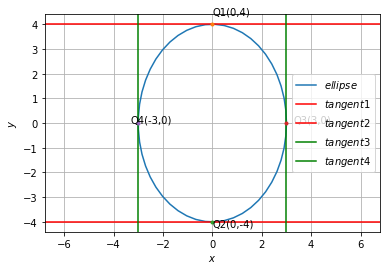
\includegraphics[width=\columnwidth]{./solutions/conics/1/16/ellipse.png}
	\caption{Figure depicting point of contact of tangents of ellipse parallel to x-axis and y-axis}
	\label{eq:solutions/1/16/fig1}
\end{figure}


\item Line segments $AD$ and $BC$ intersect at $O$ and form $\triangle OAB$ and $\triangle ODC$. $\angle  B < \angle  A$ and $\angle  C < \angle  D$. Show that $AD < BC$.

\item $AB$ and $CD$ are respectively the smallest and longest sides of a quadrilateral $ABCD$. Show that $\angle  A > \angle  C$ and $\angle  B > \angle  D$.
%
\item In $\triangle PQR,  PR > PQ$ and $PS$ bisects $\angle  QPR$. Prove that $\angle  PSR > \angle  PSQ$.
%
%\begin{enumerate}
%\renewcommand{\theequation}{\theenumi}
\begin{enumerate}[label=\thesection.\arabic*.,ref=\thesection.\theenumi]
\numberwithin{equation}{enumi}

\item The vertices of $\triangle ABC$ are taken as follows:
\label{const:table1}
\\
\solution See Table. \ref{table:table1} 
%
\begin{table}[ht!]
\centering
%%%%%%%%%%%%%%%%%%%%%%%%%%%%%%%%%%%%%%%%%%%%%%%%%%%%%%%%%%%%%%%%%%%%%%
%%                                                                  %%
%%  This is the header of a LaTeX2e file exported from Gnumeric.    %%
%%                                                                  %%
%%  This file can be compiled as it stands or included in another   %%
%%  LaTeX document. The table is based on the longtable package so  %%
%%  the longtable options (headers, footers...) can be set in the   %%
%%  preamble section below (see PRAMBLE).                           %%
%%                                                                  %%
%%  To include the file in another, the following two lines must be %%
%%  in the including file:                                          %%
%%        \def\inputGnumericTable{}                                 %%
%%  at the beginning of the file and:                               %%
%%        \input{name-of-this-file.tex}                             %%
%%  where the table is to be placed. Note also that the including   %%
%%  file must use the following packages for the table to be        %%
%%  rendered correctly:                                             %%
%%    \usepackage[latin1]{inputenc}                                 %%
%%    \usepackage{color}                                            %%
%%    \usepackage{array}                                            %%
%%    \usepackage{longtable}                                        %%
%%    \usepackage{calc}                                             %%
%%    \usepackage{multirow}                                         %%
%%    \usepackage{hhline}                                           %%
%%    \usepackage{ifthen}                                           %%
%%  optionally (for landscape tables embedded in another document): %%
%%    \usepackage{lscape}                                           %%
%%                                                                  %%
%%%%%%%%%%%%%%%%%%%%%%%%%%%%%%%%%%%%%%%%%%%%%%%%%%%%%%%%%%%%%%%%%%%%%%



%%  This section checks if we are begin input into another file or  %%
%%  the file will be compiled alone. First use a macro taken from   %%
%%  the TeXbook ex 7.7 (suggestion of Han-Wen Nienhuys).            %%
\def\ifundefined#1{\expandafter\ifx\csname#1\endcsname\relax}


%%  Check for the \def token for inputed files. If it is not        %%
%%  defined, the file will be processed as a standalone and the     %%
%%  preamble will be used.                                          %%
\ifundefined{inputGnumericTable}

%%  We must be able to close or not the document at the end.        %%
	\def\gnumericTableEnd{\end{document}}


%%%%%%%%%%%%%%%%%%%%%%%%%%%%%%%%%%%%%%%%%%%%%%%%%%%%%%%%%%%%%%%%%%%%%%
%%                                                                  %%
%%  This is the PREAMBLE. Change these values to get the right      %%
%%  paper size and other niceties.                                  %%
%%                                                                  %%
%%%%%%%%%%%%%%%%%%%%%%%%%%%%%%%%%%%%%%%%%%%%%%%%%%%%%%%%%%%%%%%%%%%%%%

	\documentclass[12pt%
			  %,landscape%
                    ]{report}
       \usepackage[latin1]{inputenc}
       \usepackage{fullpage}
       \usepackage{color}
       \usepackage{array}
       \usepackage{longtable}
       \usepackage{calc}
       \usepackage{multirow}
       \usepackage{hhline}
       \usepackage{ifthen}

	\begin{document}


%%  End of the preamble for the standalone. The next section is for %%
%%  documents which are included into other LaTeX2e files.          %%
\else

%%  We are not a stand alone document. For a regular table, we will %%
%%  have no preamble and only define the closing to mean nothing.   %%
    \def\gnumericTableEnd{}

%%  If we want landscape mode in an embedded document, comment out  %%
%%  the line above and uncomment the two below. The table will      %%
%%  begin on a new page and run in landscape mode.                  %%
%       \def\gnumericTableEnd{\end{landscape}}
%       \begin{landscape}


%%  End of the else clause for this file being \input.              %%
\fi

%%%%%%%%%%%%%%%%%%%%%%%%%%%%%%%%%%%%%%%%%%%%%%%%%%%%%%%%%%%%%%%%%%%%%%
%%                                                                  %%
%%  The rest is the gnumeric table, except for the closing          %%
%%  statement. Changes below will alter the table's appearance.     %%
%%                                                                  %%
%%%%%%%%%%%%%%%%%%%%%%%%%%%%%%%%%%%%%%%%%%%%%%%%%%%%%%%%%%%%%%%%%%%%%%

\providecommand{\gnumericmathit}[1]{#1} 
%%  Uncomment the next line if you would like your numbers to be in %%
%%  italics if they are italizised in the gnumeric table.           %%
%\renewcommand{\gnumericmathit}[1]{\mathit{#1}}
\providecommand{\gnumericPB}[1]%
{\let\gnumericTemp=\\#1\let\\=\gnumericTemp\hspace{0pt}}
 \ifundefined{gnumericTableWidthDefined}
        \newlength{\gnumericTableWidth}
        \newlength{\gnumericTableWidthComplete}
        \newlength{\gnumericMultiRowLength}
        \global\def\gnumericTableWidthDefined{}
 \fi
%% The following setting protects this code from babel shorthands.  %%
 \ifthenelse{\isundefined{\languageshorthands}}{}{\languageshorthands{english}}
%%  The default table format retains the relative column widths of  %%
%%  gnumeric. They can easily be changed to c, r or l. In that case %%
%%  you may want to comment out the next line and uncomment the one %%
%%  thereafter                                                      %%
\providecommand\gnumbox{\makebox[0pt]}
%%\providecommand\gnumbox[1][]{\makebox}

%% to adjust positions in multirow situations                       %%
\setlength{\bigstrutjot}{\jot}
\setlength{\extrarowheight}{\doublerulesep}

%%  The \setlongtables command keeps column widths the same across  %%
%%  pages. Simply comment out next line for varying column widths.  %%
\setlongtables

\setlength\gnumericTableWidth{%
	53pt+%
	53pt+%
0pt}
\def\gumericNumCols{2}
\setlength\gnumericTableWidthComplete{\gnumericTableWidth+%
         \tabcolsep*\gumericNumCols*2+\arrayrulewidth*\gumericNumCols}
\ifthenelse{\lengthtest{\gnumericTableWidthComplete > \linewidth}}%
         {\def\gnumericScale{\ratio{\linewidth-%
                        \tabcolsep*\gumericNumCols*2-%
                        \arrayrulewidth*\gumericNumCols}%
{\gnumericTableWidth}}}%
{\def\gnumericScale{1}}

%%%%%%%%%%%%%%%%%%%%%%%%%%%%%%%%%%%%%%%%%%%%%%%%%%%%%%%%%%%%%%%%%%%%%%
%%                                                                  %%
%% The following are the widths of the various columns. We are      %%
%% defining them here because then they are easier to change.       %%
%% Depending on the cell formats we may use them more than once.    %%
%%                                                                  %%
%%%%%%%%%%%%%%%%%%%%%%%%%%%%%%%%%%%%%%%%%%%%%%%%%%%%%%%%%%%%%%%%%%%%%%

\ifthenelse{\isundefined{\gnumericColA}}{\newlength{\gnumericColA}}{}\settowidth{\gnumericColA}{\begin{tabular}{@{}p{53pt*\gnumericScale}@{}}x\end{tabular}}
\ifthenelse{\isundefined{\gnumericColB}}{\newlength{\gnumericColB}}{}\settowidth{\gnumericColB}{\begin{tabular}{@{}p{53pt*\gnumericScale}@{}}x\end{tabular}}

\begin{tabular}[c]{%
	b{\gnumericColA}%
	b{\gnumericColB}%
	}

%%%%%%%%%%%%%%%%%%%%%%%%%%%%%%%%%%%%%%%%%%%%%%%%%%%%%%%%%%%%%%%%%%%%%%
%%  The longtable options. (Caption, headers... see Goosens, p.124) %%
%	\caption{The Table Caption.}             \\	%
% \hline	% Across the top of the table.
%%  The rest of these options are table rows which are placed on    %%
%%  the first, last or every page. Use \multicolumn if you want.    %%

%%  Header for the first page.                                      %%
%	\multicolumn{2}{c}{The First Header} \\ \hline 
%	\multicolumn{1}{c}{colTag}	%Column 1
%	&\multicolumn{1}{c}{colTag}	\\ \hline %Last column
%	\endfirsthead

%%  The running header definition.                                  %%
%	\hline
%	\multicolumn{2}{l}{\ldots\small\slshape continued} \\ \hline
%	\multicolumn{1}{c}{colTag}	%Column 1
%	&\multicolumn{1}{c}{colTag}	\\ \hline %Last column
%	\endhead

%%  The running footer definition.                                  %%
%	\hline
%	\multicolumn{2}{r}{\small\slshape continued\ldots} \\
%	\endfoot

%%  The ending footer definition.                                   %%
%	\multicolumn{2}{c}{That's all folks} \\ \hline 
%	\endlastfoot
%%%%%%%%%%%%%%%%%%%%%%%%%%%%%%%%%%%%%%%%%%%%%%%%%%%%%%%%%%%%%%%%%%%%%%

\hhline{|--}
	 \multicolumn{2}{|p{	\gnumericColA+%
	\gnumericColB+%
	\tabcolsep*2*1}|}%
	{\gnumericPB{\centering}\gnumbox{\textbf{Initial Input Values}}}
\\
\hhline{|-|-|}
	 \multicolumn{1}{|p{\gnumericColA}|}%
	{\gnumericPB{\centering}\gnumbox{\textbf{Parameter}}}
	&\multicolumn{1}{p{\gnumericColB}|}%
	{\gnumericPB{\centering}\gnumbox{\textbf{Value}}}
\\
\hhline{|--|}
	 \multicolumn{1}{|p{\gnumericColA}|}%
	{\gnumericPB{\centering}\gnumbox{\textbf{a}}}
	&\multicolumn{1}{p{\gnumericColB}|}%
	{\gnumericPB{\centering}\gnumbox{\textbf{4}}}
\\
\hhline{|--|}
	 \multicolumn{1}{|p{\gnumericColA}|}%
	{\gnumericPB{\centering}\gnumbox{\textbf{b}}}
	&\multicolumn{1}{p{\gnumericColB}|}%
	{\gnumericPB{\centering}\gnumbox{\textbf{4}}}
\\
\hhline{|--|}
	 \multicolumn{1}{|p{\gnumericColA}|}%
	{\gnumericPB{\centering}\gnumbox{\textbf{c}}}
	&\multicolumn{1}{p{\gnumericColB}|}%
	{\gnumericPB{\centering}\gnumbox{\textbf{4}}}
\\
\hhline{|-|-|}
\end{tabular}

\ifthenelse{\isundefined{\languageshorthands}}{}{\languageshorthands{\languagename}}
\gnumericTableEnd

\caption{To construct triangle ABC}
\label{table:table1}	
\end{table}

%\item

\item The midpoints of sides are given as
\begin{align}
\vec{D} &= \frac{\vec{B}+\vec{C}}{2}
\label{eq:pointd}
\\
\vec{E} &= \frac{\vec{A}+\vec{C}}{2}
\\
\vec{F} &= \frac{\vec{A}+\vec{B}}{2}
\end{align}
\item Also Centroid divides median in ratio 2:1.So by section formulae $\vec{O}$ is given as
\begin{align}
\vec{O} &= \frac{2\vec{D}+\vec{A}}{3}
\label{eq:centr}
\end{align}

The derived coordinates are listed in \ref{table:table2}. 
%
\begin{table}[ht!]
\centering
%%%%%%%%%%%%%%%%%%%%%%%%%%%%%%%%%%%%%%%%%%%%%%%%%%%%%%%%%%%%%%%%%%%%%%
%%                                                                  %%
%%  This is the header of a LaTeX2e file exported from Gnumeric.    %%
%%                                                                  %%
%%  This file can be compiled as it stands or included in another   %%
%%  LaTeX document. The table is based on the longtable package so  %%
%%  the longtable options (headers, footers...) can be set in the   %%
%%  preamble section below (see PRAMBLE).                           %%
%%                                                                  %%
%%  To include the file in another, the following two lines must be %%
%%  in the including file:                                          %%
%%        \def\inputGnumericTable{}                                 %%
%%  at the beginning of the file and:                               %%
%%        \input{name-of-this-file.tex}                             %%
%%  where the table is to be placed. Note also that the including   %%
%%  file must use the following packages for the table to be        %%
%%  rendered correctly:                                             %%
%%    \usepackage[latin1]{inputenc}                                 %%
%%    \usepackage{color}                                            %%
%%    \usepackage{array}                                            %%
%%    \usepackage{longtable}                                        %%
%%    \usepackage{calc}                                             %%
%%    \usepackage{multirow}                                         %%
%%    \usepackage{hhline}                                           %%
%%    \usepackage{ifthen}                                           %%
%%  optionally (for landscape tables embedded in another document): %%
%%    \usepackage{lscape}                                           %%
%%                                                                  %%
%%%%%%%%%%%%%%%%%%%%%%%%%%%%%%%%%%%%%%%%%%%%%%%%%%%%%%%%%%%%%%%%%%%%%%



%%  This section checks if we are begin input into another file or  %%
%%  the file will be compiled alone. First use a macro taken from   %%
%%  the TeXbook ex 7.7 (suggestion of Han-Wen Nienhuys).            %%
\def\ifundefined#1{\expandafter\ifx\csname#1\endcsname\relax}


%%  Check for the \def token for inputed files. If it is not        %%
%%  defined, the file will be processed as a standalone and the     %%
%%  preamble will be used.                                          %%
\ifundefined{inputGnumericTable}

%%  We must be able to close or not the document at the end.        %%
	\def\gnumericTableEnd{\end{document}}


%%%%%%%%%%%%%%%%%%%%%%%%%%%%%%%%%%%%%%%%%%%%%%%%%%%%%%%%%%%%%%%%%%%%%%
%%                                                                  %%
%%  This is the PREAMBLE. Change these values to get the right      %%
%%  paper size and other niceties.                                  %%
%%                                                                  %%
%%%%%%%%%%%%%%%%%%%%%%%%%%%%%%%%%%%%%%%%%%%%%%%%%%%%%%%%%%%%%%%%%%%%%%

	\documentclass[12pt%
			  %,landscape%
                    ]{report}
       \usepackage[latin1]{inputenc}
       \usepackage{fullpage}
       \usepackage{color}
       \usepackage{array}
       \usepackage{longtable}
       \usepackage{calc}
       \usepackage{multirow}
       \usepackage{hhline}
       \usepackage{ifthen}

	\begin{document}


%%  End of the preamble for the standalone. The next section is for %%
%%  documents which are included into other LaTeX2e files.          %%
\else

%%  We are not a stand alone document. For a regular table, we will %%
%%  have no preamble and only define the closing to mean nothing.   %%
    \def\gnumericTableEnd{}

%%  If we want landscape mode in an embedded document, comment out  %%
%%  the line above and uncomment the two below. The table will      %%
%%  begin on a new page and run in landscape mode.                  %%
%       \def\gnumericTableEnd{\end{landscape}}
%       \begin{landscape}


%%  End of the else clause for this file being \input.              %%
\fi

%%%%%%%%%%%%%%%%%%%%%%%%%%%%%%%%%%%%%%%%%%%%%%%%%%%%%%%%%%%%%%%%%%%%%%
%%                                                                  %%
%%  The rest is the gnumeric table, except for the closing          %%
%%  statement. Changes below will alter the table's appearance.     %%
%%                                                                  %%
%%%%%%%%%%%%%%%%%%%%%%%%%%%%%%%%%%%%%%%%%%%%%%%%%%%%%%%%%%%%%%%%%%%%%%

\providecommand{\gnumericmathit}[1]{#1} 
%%  Uncomment the next line if you would like your numbers to be in %%
%%  italics if they are italizised in the gnumeric table.           %%
%\renewcommand{\gnumericmathit}[1]{\mathit{#1}}
\providecommand{\gnumericPB}[1]%
{\let\gnumericTemp=\\#1\let\\=\gnumericTemp\hspace{0pt}}
 \ifundefined{gnumericTableWidthDefined}
        \newlength{\gnumericTableWidth}
        \newlength{\gnumericTableWidthComplete}
        \newlength{\gnumericMultiRowLength}
        \global\def\gnumericTableWidthDefined{}
 \fi
%% The following setting protects this code from babel shorthands.  %%
 \ifthenelse{\isundefined{\languageshorthands}}{}{\languageshorthands{english}}
%%  The default table format retains the relative column widths of  %%
%%  gnumeric. They can easily be changed to c, r or l. In that case %%
%%  you may want to comment out the next line and uncomment the one %%
%%  thereafter                                                      %%
\providecommand\gnumbox{\makebox[0pt]}
%%\providecommand\gnumbox[1][]{\makebox}

%% to adjust positions in multirow situations                       %%
\setlength{\bigstrutjot}{\jot}
\setlength{\extrarowheight}{\doublerulesep}

%%  The \setlongtables command keeps column widths the same across  %%
%%  pages. Simply comment out next line for varying column widths.  %%
\setlongtables

\setlength\gnumericTableWidth{%
	50pt+%
	75pt+%
0pt}
\def\gumericNumCols{2}
\setlength\gnumericTableWidthComplete{\gnumericTableWidth+%
         \tabcolsep*\gumericNumCols*2+\arrayrulewidth*\gumericNumCols}
\ifthenelse{\lengthtest{\gnumericTableWidthComplete > \linewidth}}%
         {\def\gnumericScale{\ratio{\linewidth-%
                        \tabcolsep*\gumericNumCols*2-%
                        \arrayrulewidth*\gumericNumCols}%
{\gnumericTableWidth}}}%
{\def\gnumericScale{1}}

%%%%%%%%%%%%%%%%%%%%%%%%%%%%%%%%%%%%%%%%%%%%%%%%%%%%%%%%%%%%%%%%%%%%%%
%%                                                                  %%
%% The following are the widths of the various columns. We are      %%
%% defining them here because then they are easier to change.       %%
%% Depending on the cell formats we may use them more than once.    %%
%%                                                                  %%
%%%%%%%%%%%%%%%%%%%%%%%%%%%%%%%%%%%%%%%%%%%%%%%%%%%%%%%%%%%%%%%%%%%%%%

\ifthenelse{\isundefined{\gnumericColA}}{\newlength{\gnumericColA}}{}\settowidth{\gnumericColA}{\begin{tabular}{@{}p{50pt*\gnumericScale}@{}}x\end{tabular}}
\ifthenelse{\isundefined{\gnumericColB}}{\newlength{\gnumericColB}}{}\settowidth{\gnumericColB}{\begin{tabular}{@{}p{75pt*\gnumericScale}@{}}x\end{tabular}}

\begin{tabular}[c]{%
	b{\gnumericColA}%
	b{\gnumericColB}%
	}

%%%%%%%%%%%%%%%%%%%%%%%%%%%%%%%%%%%%%%%%%%%%%%%%%%%%%%%%%%%%%%%%%%%%%%
%%  The longtable options. (Caption, headers... see Goosens, p.124) %%
%	\caption{The Table Caption.}             \\	%
% \hline	% Across the top of the table.
%%  The rest of these options are table rows which are placed on    %%
%%  the first, last or every page. Use \multicolumn if you want.    %%

%%  Header for the first page.                                      %%
%	\multicolumn{2}{c}{The First Header} \\ \hline 
%	\multicolumn{1}{c}{colTag}	%Column 1
%	&\multicolumn{1}{c}{colTag}	\\ \hline %Last column
%	\endfirsthead

%%  The running header definition.                                  %%
%	\hline
%	\multicolumn{2}{l}{\ldots\small\slshape continued} \\ \hline
%	\multicolumn{1}{c}{colTag}	%Column 1
%	&\multicolumn{1}{c}{colTag}	\\ \hline %Last column
%	\endhead

%%  The running footer definition.                                  %%
%	\hline
%	\multicolumn{2}{r}{\small\slshape continued\ldots} \\
%	\endfoot

%%  The ending footer definition.                                   %%
%	\multicolumn{2}{c}{That's all folks} \\ \hline 
%	\endlastfoot
%%%%%%%%%%%%%%%%%%%%%%%%%%%%%%%%%%%%%%%%%%%%%%%%%%%%%%%%%%%%%%%%%%%%%%

\hhline{|-|-}
	 \multicolumn{1}{|p{\gnumericColA}|}%
	{\gnumericPB{\raggedright}\gnumbox[l]{Vector}}
	&\multicolumn{1}{p{\gnumericColB}|}%
	{\gnumericPB{\raggedright}\gnumbox[l]{Coordinates}}
\\
\hhline{|--|}
	 \multicolumn{1}{|p{\gnumericColA}|}%
	{\gnumericPB{\centering}\gnumbox{\textbf{D}}}
	&\multicolumn{1}{p{\gnumericColB}|}%
	{\gnumericPB{\centering}\gnumbox{$\myvec{3\\1}$}}
\\
\hhline{|--|}
	 \multicolumn{1}{|p{\gnumericColA}|}%
	{\gnumericPB{\centering}\gnumbox{\textbf{E}}}
	&\multicolumn{1}{p{\gnumericColB}|}%
	{\gnumericPB{\centering}\gnumbox{$\myvec{2\\0}$}}
\\
\hhline{|--|}
	 \multicolumn{1}{|p{\gnumericColA}|}%
	{\gnumericPB{\centering}\gnumbox{\textbf{F}}}
	&\multicolumn{1}{p{\gnumericColB}|}%
	{\gnumericPB{\centering}\gnumbox{$\myvec{1\\1}$}}
\\
\hhline{|--|}
	 \multicolumn{1}{|p{\gnumericColA}|}%
	{\gnumericPB{\centering}\gnumbox{\textbf{O}}}
	&\multicolumn{1}{p{\gnumericColB}|}%
	{\gnumericPB{\centering}\gnumbox{$\myvec{3\\\frac{2}{3}}$}}
\\
\hhline{|-|-|}
\end{tabular}

\ifthenelse{\isundefined{\languageshorthands}}{}{\languageshorthands{\languagename}}
\gnumericTableEnd

\caption{Derived coordinates of triangle ABC}
\label{table:table2}	
\end{table}

\end{enumerate}

%
General equation of conics is 
\begin{align}
    \vec{x}^T\vec{V}\vec{x}+ 2\vec{u}^T\vec{x}+f = 0
    \label{eq:solutions/1/16/eq:1}
\end{align}
Comparing with the equation given,
\begin{align}
\vec{V}=\myvec{\frac{1}{9} & 0 \\ 0 & \frac{1}{16}}\\
\vec{u}=\vec{0}\\
f=-1\\
\mydet{\vec{v}}=\mydet{\myvec{\frac{1}{9} & 0 \\ 0 & \frac{1}{16}}}>0
\end{align}
$\because \abs{\vec{V}}>0$, the given equation is of ellipse.\\
a)The tangents are parallel to the x-axis, hence, their direction and normal vectors, $\vec{m_1}$ and $\vec{n_1}$ are respectively,
\begin{align}
\vec{m_1}=\myvec{1\\0}\\
\vec{n_1}=\myvec{0\\1}
\end{align}
For an ellipse, given the normal vector $\vec{n}$, the tangent points of contact to the ellipse are given by
\begin{align}
    \vec{q}=\vec{V}^{-1}(\kappa \vec{n}-\vec{u})
    \label{eq:solutions/1/16/eq:2}
    =\vec{V}^{-1}\kappa \vec{n}
\end{align}
where
\begin{align}
    \kappa=\pm \sqrt{\frac{\vec{u^T}\vec{V}^{-1}\vec{u}-f}{\vec{n^T}\vec{V}^{-1}\vec{n}}}
    \label{eq:solutions/1/16/eq:2.0.9}\\
   =\pm \sqrt{\frac{-f}{\vec{n^T}\vec{V}^{-1}\vec{n}}}\\
    \vec{V}^{-1}=\myvec{9 & 0 \\ 0 & 16}\\
    \kappa_1=\pm \sqrt{\frac{-(-1)}{\myvec{0 & 1}\myvec{9 & 0 \\ 0 & 16} \myvec{0\\1}}}\\
 \implies \kappa_1=\pm \sqrt{\frac{1}{16}}\\
    \implies \kappa_1=\pm \frac{1}{4}      
\end{align}
From \eqref{eq:solutions/1/16/eq:2} , the point of contact $\vec{q_i}$ are,
\begin{align}
    \vec{q_1}=\myvec{9 & 0 \\ 0 & 16}\frac{1}{4}\myvec{0\\1}\\
    =\myvec{9 & 0 \\ 0 & 16}\myvec{0\\\frac{1}{4}}\\
    =\myvec{0\\4}\\
    \vec{q_2}=\myvec{9 & 0 \\ 0 & 16}\left(-\frac{1}{4}\right)\ \myvec{0\\1}\\
    =\myvec{9 & 0 \\ 0 & 16}\myvec{0\\-\frac{1}{4}}\\
    =\myvec{0\\-4}
\end{align}
b) The tangents are parallel to the y-axis, hence, their direction and normal vectors, $\vec{m_2}$ and $\vec{n_2}$ are respectively,
\begin{align}
\vec{m_2}=\myvec{0\\1}\\
\vec{n_2}=\myvec{1\\0}
\end{align}
Using equation \eqref{eq:solutions/1/16/eq:2.0.9}, the values of $\kappa$ for this case are
\begin{align}
     \kappa_2=\pm \sqrt{\frac{-(-1)}{\myvec{1 & 0}\myvec{9 & 0 \\ 0 & 16} \myvec{1\\0}}}\\
 \implies \kappa_2=\pm \sqrt{\frac{1}{9}}\\
    \implies \kappa_2=\pm \frac{1}{3} 
\end{align}
and from \eqref{eq:solutions/1/16/eq:2} , the point of contact $\vec{q_i}$ are,
\begin{align}
\vec{q_3}=\myvec{9 & 0 \\ 0 & 16}\frac{1}{3}\myvec{1\\0}\\
    =\myvec{9 & 0 \\ 0 & 16}\myvec{\frac{1}{3}\\0}\\
    =\myvec{3\\0}\\
\vec{q_4}=\myvec{9 & 0 \\ 0 & 16}\left(-\frac{1}{3}\right)\ \myvec{1\\0}\\
    =\myvec{9 & 0 \\ 0 & 16}\myvec{-\frac{1}{3}\\0}\\
    =\myvec{-3\\0}
\end{align}
 \begin{figure}[h!]
	\centering
	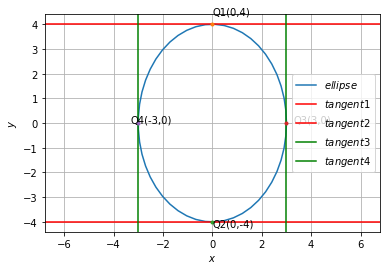
\includegraphics[width=\columnwidth]{./solutions/conics/1/16/ellipse.png}
	\caption{Figure depicting point of contact of tangents of ellipse parallel to x-axis and y-axis}
	\label{eq:solutions/1/16/fig1}
\end{figure}

%\end{enumerate}

\item Show that of all line segments drawn from a given point not on it, the perpendicular line segment is the shortest.
%
\item $ABCD$ is a trapezium with $AB  \parallel  DC$. $E$ and $F$ are points on non-parallel sides $AD$ and $BC$ respectively such that $EF$ is parallel to $AB$
. Show that
$\frac{AE}{ED}=\frac{ BF}{  FC}$ .
%\begin{enumerate}
%
%\renewcommand{\thefigure}{\theenumi.\arabic{figure}}
\begin{figure}[!ht]
\centering
\resizebox{\columnwidth}{!}{\renewcommand{\theequation}{\theenumi}
\begin{enumerate}[label=\thesection.\arabic*.,ref=\thesection.\theenumi]
\numberwithin{equation}{enumi}
\item  Find the centre and radius of the circle 
\begin{align}
x^2+y^2+8x+10y-8 = 0
\label{eq:circ_basic}
\end{align}
\solution
\eqref{eq:circ_basic} can be expressed as 
\begin{align}
\vec{x}^T\vec{x}+ 2\myvec{4 & 5}\vec{x} -8 = 0
\end{align}
which is of the form \eqref{eq:conic_quad_form} with
\begin{align}
\label{eq:circ_basic_uf}
\vec{u} = \myvec{4\\5}, f = -8
\end{align}
From  Table \ref{table:conics}, the center and radius are given by 
\begin{align}
\vec{c} = -\vec{u} = \myvec{-4\\-5},
r = \sqrt{\norm{u}^2-f} = 7
\end{align}
\item Find the equation of a circle which passes through the points $\vec{P} = \myvec{2\\-2}$ and $\vec{Q} = \myvec{3\\4}$ and whose centre lies on the line  
%\cite{eleven}
\begin{align}
\label{eq:circ_ex1_line}
\myvec{1 & 1} \vec{x} = 2
\end{align}
\solution From \eqref{eq:conic_quad_form} and Table \ref{table:conics}, the equation of a circle can be expressed as
\begin{align}
\label{eq:circ_conic}
\vec{x}^T\vec{x}-2\vec{c}^T\vec{x}+f = 0
\end{align}
where $\vec{c}$ is the centre.
Substituting the given points in 
\eqref{eq:circ_conic} and using 
\eqref{eq:circ_ex1_line}, the following equations are obtained
\begin{align}
2\myvec{2 & -2}\vec{c} -  f &= 8
\\
2\myvec{3 & 4}\vec{c} -  f &= 25
\\
\myvec{1 & 1}\vec{c}  &= 2
\end{align}
which can be expressed as the matrix equation
\begin{align}
\myvec{
1 & 1 & 0
\\
4 & -4 & -1 
\\ 
6 & 8 & -1  
}
\myvec{\vec{c}\\f} = \myvec{2\\8\\25}
\end{align}
Row reducing the augmented matrix
\begin{align}
\myvec{
1 & 1 & 0 & 2
\\
4 & -4 & -1 & 8
\\ 
6 & 8 & -1  & 25
}
\\
\xleftrightarrow[R_3 \leftarrow R_3 -6R_1]{R_2 \leftarrow -R_2+4R_1}
\myvec{
1 & 1 & 0 & 2
\\
0 & 8 & 1 & 0
\\ 
0 & 2 & -1  & 13
}
\\
\xleftrightarrow[R_3 \leftarrow -\frac{4R_3 -R_2}{2}]{R_1 \leftarrow 8R_1-R_3}
\myvec{
8 & 0 & -1 & 16
\\
0 & 8 & 1 & 0
\\ 
0 & 0 & 5  & -52
}
\\
\xleftrightarrow[R_2 \leftarrow \frac{5R_2 -R_3}{4}]{R_1 \leftarrow \frac{5R_1+R_3}{4}}
\myvec{
10 & 0 & 0 & 7
\\
0 & 10 & 0 & 13
\\ 
0 & 0 & 5  & -52
}
\end{align}
Thus, 
\begin{align}
\vec{c} &= \frac{1}{10}\myvec{7\\13}
\\
f &=-\frac{52}{5}
\end{align}
which give the desired equation of the circle.
From Table \ref{table:conics},
%
\begin{align}
 r =  \sqrt{\norm{\vec{c}}^2-f} = \frac{1}{10}\sqrt{1258}
\end{align}
Fig. \ref{fig:CircOr}	verifies the above results.

\begin{figure}[!ht]
\centering
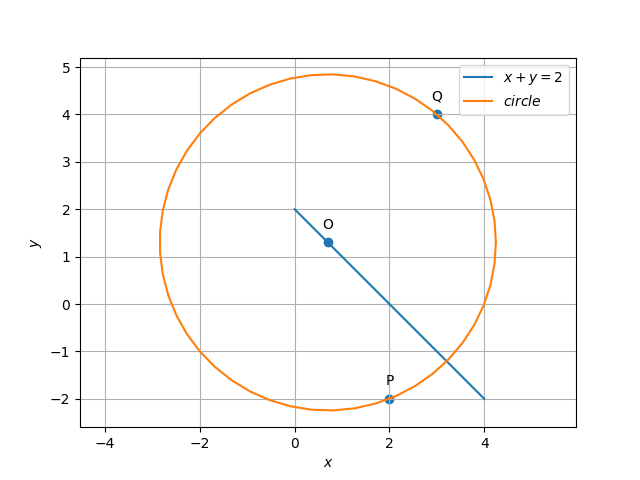
\includegraphics[width=\columnwidth]{./figs/circex/CircOr.eps}
\caption{Circle passing through $\myvec{2\\-2},\myvec{3\\4}$. Center is on line $\myvec{1 & 1}\vec{x}=2$. }
\label{fig:CircOr}	
\end{figure}

\item 
Find the points on the curve  
%\cite{twelve_one}
\begin{align}
x^2+y^2-2x-3 = 0
\label{eq:circle_tangent_prob}
\end{align}
at which the tangents are parallel to the $x$-axis.
\\
\solution \eqref{eq:circle_tangent_prob} can be expressed as
\begin{align}
\vec{x}^T\vec{x}+\myvec{-2 & 0}\vec{x}-3 &= 0
\label{eq:circle_tangent_prob_vec}
\\
\implies \vec{V} = \vec{I}, \vec{u} = \myvec{-1 \\ 0}, f = -3
\label{eq:circle_tangent_prob_uf}
\end{align}
From Table \ref{table:conics}, the centre and radius are
\begin{align}
\vec{c} = -\vec{u} = \myvec{-1 \\ 0}, r =\sqrt{\norm{\vec{u}}^2-f} = 2
\end{align}
$\because$ the tangents are parallel to the $x$-axis, their direction and normal vectors are respectively,
\begin{align}
\vec{m} = \myvec{1\\0},
\vec{n} = \myvec{0\\1}.
\end{align}
From Table \ref{table:conics},
\begin{align}
\kappa = \pm \sqrt{\frac{\vec{u}^T\vec{u}-f}{\vec{n}^T\vec{n}}} = \pm \sqrt{\frac{4}{1}} = \pm 2
\end{align}
and the desired points of contact are 
\begin{align}
\vec{q}_1, \vec{q}_2 = \myvec{1\\0}\pm 2\myvec{0\\1} =  
\myvec{1 \\  2},
\myvec{1 \\  -2}
\end{align}
%
Fig. \ref{fig:CircOr}	verifies the above results.
\begin{figure}[!ht]
\centering
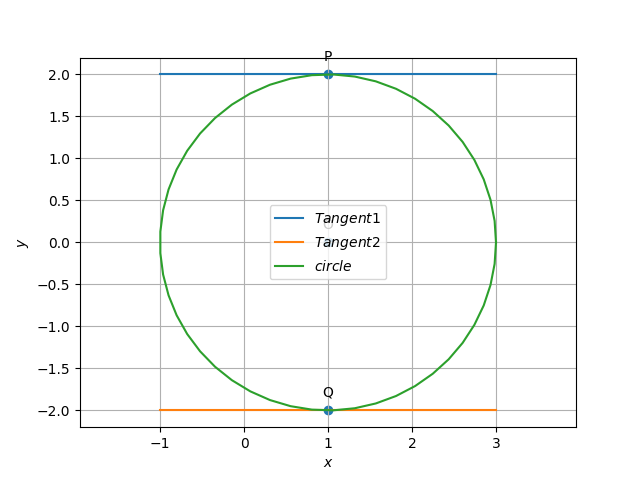
\includegraphics[width=\columnwidth]{./figs/circex/CircTangent.eps}
\caption{Tangents are parallel to the $x$-axis. }
\label{fig:CircTangent}	
\end{figure}

\end{enumerate}
}
\caption{}
\label{fig:8.5.16_circle_latex}	
\end{figure}
%
%
%\renewcommand{\thefigure}{\theenumi}
%
\item {\em Construction: }In Fig. \ref{fig:8.5.16_circle_latex} the known parameters are
%\label{}
\\
%
%\solution From the given information, 
%$\triangle ABC$ are 
\begin{align}
\vec{O} &= \myvec{0\\0} ,
\\
\vec{A} &= \myvec{r\\0} ,
\label{eq:8.5.16_constr_a}
\\
 \vec{B} &= \myvec{-r\\0} 
\label{eq:8.5.16_constr_b}
\\
\vec{C}&= r\myvec{\cos\theta\\\sin\theta}
\label{eq:8.5.16_constr_cgen}
\end{align}
%
Let 
\begin{align}
\vec{D} & = r\myvec{\cos\theta_1\\\sin\theta_1} 
\label{eq:8.5.16_constr_dgen}
\end{align}
From the given information,
\begin{align}
 \norm{\vec{D} - \vec{C}} &= r
\\
\implies \brak{\vec{D} - \vec{C}}^T\brak{\vec{D} - \vec{C}} &= r^2\\
 \label{eq:8.5.16_dist_formula}
\\
\implies  \norm{D} ^2 - 2\vec{D}^T\vec{C} +  \norm{C}^2 &=r^2 
\end{align}
In the above, 
\begin{align}
\because \norm{D} &= \norm{\vec{C}} = r,
\\
\frac{\vec{D}^T\vec{C}}{\norm{D}\norm{C}}  &= \frac{1}{2}
\\
\implies \cos \brak{\theta_1-\theta} &= 60 \degree
\label{eq:8.5.16_theta_diff}
\end{align}
using the definition of the inner product.  $\because \theta$ is known, we get $\theta_1$ from \eqref{eq:8.5.16_theta_diff}
and $\vec{D}$ from 
\eqref{eq:8.5.16_constr_dgen}. 
%
\subitem Thus,
\begin{align}
BD: \vec{x} &= \vec{B} + \lambda_1 \brak{\vec{B}-\vec{D}}
\\
AC: \vec{x} &= \vec{A} + \lambda_2 \brak{\vec{A}-\vec{C}}
\end{align}
%
which can be used to obtain $\vec{E}$.


%
General equation of conics is 
\begin{align}
    \vec{x}^T\vec{V}\vec{x}+ 2\vec{u}^T\vec{x}+f = 0
    \label{eq:solutions/1/16/eq:1}
\end{align}
Comparing with the equation given,
\begin{align}
\vec{V}=\myvec{\frac{1}{9} & 0 \\ 0 & \frac{1}{16}}\\
\vec{u}=\vec{0}\\
f=-1\\
\mydet{\vec{v}}=\mydet{\myvec{\frac{1}{9} & 0 \\ 0 & \frac{1}{16}}}>0
\end{align}
$\because \abs{\vec{V}}>0$, the given equation is of ellipse.\\
a)The tangents are parallel to the x-axis, hence, their direction and normal vectors, $\vec{m_1}$ and $\vec{n_1}$ are respectively,
\begin{align}
\vec{m_1}=\myvec{1\\0}\\
\vec{n_1}=\myvec{0\\1}
\end{align}
For an ellipse, given the normal vector $\vec{n}$, the tangent points of contact to the ellipse are given by
\begin{align}
    \vec{q}=\vec{V}^{-1}(\kappa \vec{n}-\vec{u})
    \label{eq:solutions/1/16/eq:2}
    =\vec{V}^{-1}\kappa \vec{n}
\end{align}
where
\begin{align}
    \kappa=\pm \sqrt{\frac{\vec{u^T}\vec{V}^{-1}\vec{u}-f}{\vec{n^T}\vec{V}^{-1}\vec{n}}}
    \label{eq:solutions/1/16/eq:2.0.9}\\
   =\pm \sqrt{\frac{-f}{\vec{n^T}\vec{V}^{-1}\vec{n}}}\\
    \vec{V}^{-1}=\myvec{9 & 0 \\ 0 & 16}\\
    \kappa_1=\pm \sqrt{\frac{-(-1)}{\myvec{0 & 1}\myvec{9 & 0 \\ 0 & 16} \myvec{0\\1}}}\\
 \implies \kappa_1=\pm \sqrt{\frac{1}{16}}\\
    \implies \kappa_1=\pm \frac{1}{4}      
\end{align}
From \eqref{eq:solutions/1/16/eq:2} , the point of contact $\vec{q_i}$ are,
\begin{align}
    \vec{q_1}=\myvec{9 & 0 \\ 0 & 16}\frac{1}{4}\myvec{0\\1}\\
    =\myvec{9 & 0 \\ 0 & 16}\myvec{0\\\frac{1}{4}}\\
    =\myvec{0\\4}\\
    \vec{q_2}=\myvec{9 & 0 \\ 0 & 16}\left(-\frac{1}{4}\right)\ \myvec{0\\1}\\
    =\myvec{9 & 0 \\ 0 & 16}\myvec{0\\-\frac{1}{4}}\\
    =\myvec{0\\-4}
\end{align}
b) The tangents are parallel to the y-axis, hence, their direction and normal vectors, $\vec{m_2}$ and $\vec{n_2}$ are respectively,
\begin{align}
\vec{m_2}=\myvec{0\\1}\\
\vec{n_2}=\myvec{1\\0}
\end{align}
Using equation \eqref{eq:solutions/1/16/eq:2.0.9}, the values of $\kappa$ for this case are
\begin{align}
     \kappa_2=\pm \sqrt{\frac{-(-1)}{\myvec{1 & 0}\myvec{9 & 0 \\ 0 & 16} \myvec{1\\0}}}\\
 \implies \kappa_2=\pm \sqrt{\frac{1}{9}}\\
    \implies \kappa_2=\pm \frac{1}{3} 
\end{align}
and from \eqref{eq:solutions/1/16/eq:2} , the point of contact $\vec{q_i}$ are,
\begin{align}
\vec{q_3}=\myvec{9 & 0 \\ 0 & 16}\frac{1}{3}\myvec{1\\0}\\
    =\myvec{9 & 0 \\ 0 & 16}\myvec{\frac{1}{3}\\0}\\
    =\myvec{3\\0}\\
\vec{q_4}=\myvec{9 & 0 \\ 0 & 16}\left(-\frac{1}{3}\right)\ \myvec{1\\0}\\
    =\myvec{9 & 0 \\ 0 & 16}\myvec{-\frac{1}{3}\\0}\\
    =\myvec{-3\\0}
\end{align}
 \begin{figure}[h!]
	\centering
	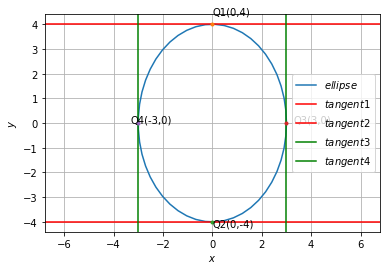
\includegraphics[width=\columnwidth]{./solutions/conics/1/16/ellipse.png}
	\caption{Figure depicting point of contact of tangents of ellipse parallel to x-axis and y-axis}
	\label{eq:solutions/1/16/fig1}
\end{figure}

%\end{enumerate}

\item $ST$ is a line joining two points on $PQ$ and $PR$ in $\triangle PQR$.  If $\frac{PS}{ SQ}=\frac{PT}{ TR}$ and $ \angle  PST = \angle  PRQ$, prove that $PQR$ is an isosceles triangle.
%
\item If $LM  \parallel  CB$ and $LN  \parallel  CD$, prove that $\frac{AM}{AB} = \frac{ AN}{AD}$.
%
\item $D$ is a point on $AB$ and $E, F$ are points on $BC$ such that $DE  \parallel  AC$ and $DF  \parallel  AE$. Prove that $\frac{BF} {FE} =\frac{BE}  {EC}$.
%
\item $O$ is a point in the interior of $\triangle ABC$. $D$ is a point on $OA$.  If $DE  \parallel  OB$ and $DF  \parallel  OC$. Show that $EF  \parallel  BC$.
%\begin{enumerate}
%
%\renewcommand{\thefigure}{\theenumi.\arabic{figure}}
\begin{figure}[!ht]
\centering
\resizebox{\columnwidth}{!}{\renewcommand{\theequation}{\theenumi}
\begin{enumerate}[label=\thesection.\arabic*.,ref=\thesection.\theenumi]
\numberwithin{equation}{enumi}
\item  Find the centre and radius of the circle 
\begin{align}
x^2+y^2+8x+10y-8 = 0
\label{eq:circ_basic}
\end{align}
\solution
\eqref{eq:circ_basic} can be expressed as 
\begin{align}
\vec{x}^T\vec{x}+ 2\myvec{4 & 5}\vec{x} -8 = 0
\end{align}
which is of the form \eqref{eq:conic_quad_form} with
\begin{align}
\label{eq:circ_basic_uf}
\vec{u} = \myvec{4\\5}, f = -8
\end{align}
From  Table \ref{table:conics}, the center and radius are given by 
\begin{align}
\vec{c} = -\vec{u} = \myvec{-4\\-5},
r = \sqrt{\norm{u}^2-f} = 7
\end{align}
\item Find the equation of a circle which passes through the points $\vec{P} = \myvec{2\\-2}$ and $\vec{Q} = \myvec{3\\4}$ and whose centre lies on the line  
%\cite{eleven}
\begin{align}
\label{eq:circ_ex1_line}
\myvec{1 & 1} \vec{x} = 2
\end{align}
\solution From \eqref{eq:conic_quad_form} and Table \ref{table:conics}, the equation of a circle can be expressed as
\begin{align}
\label{eq:circ_conic}
\vec{x}^T\vec{x}-2\vec{c}^T\vec{x}+f = 0
\end{align}
where $\vec{c}$ is the centre.
Substituting the given points in 
\eqref{eq:circ_conic} and using 
\eqref{eq:circ_ex1_line}, the following equations are obtained
\begin{align}
2\myvec{2 & -2}\vec{c} -  f &= 8
\\
2\myvec{3 & 4}\vec{c} -  f &= 25
\\
\myvec{1 & 1}\vec{c}  &= 2
\end{align}
which can be expressed as the matrix equation
\begin{align}
\myvec{
1 & 1 & 0
\\
4 & -4 & -1 
\\ 
6 & 8 & -1  
}
\myvec{\vec{c}\\f} = \myvec{2\\8\\25}
\end{align}
Row reducing the augmented matrix
\begin{align}
\myvec{
1 & 1 & 0 & 2
\\
4 & -4 & -1 & 8
\\ 
6 & 8 & -1  & 25
}
\\
\xleftrightarrow[R_3 \leftarrow R_3 -6R_1]{R_2 \leftarrow -R_2+4R_1}
\myvec{
1 & 1 & 0 & 2
\\
0 & 8 & 1 & 0
\\ 
0 & 2 & -1  & 13
}
\\
\xleftrightarrow[R_3 \leftarrow -\frac{4R_3 -R_2}{2}]{R_1 \leftarrow 8R_1-R_3}
\myvec{
8 & 0 & -1 & 16
\\
0 & 8 & 1 & 0
\\ 
0 & 0 & 5  & -52
}
\\
\xleftrightarrow[R_2 \leftarrow \frac{5R_2 -R_3}{4}]{R_1 \leftarrow \frac{5R_1+R_3}{4}}
\myvec{
10 & 0 & 0 & 7
\\
0 & 10 & 0 & 13
\\ 
0 & 0 & 5  & -52
}
\end{align}
Thus, 
\begin{align}
\vec{c} &= \frac{1}{10}\myvec{7\\13}
\\
f &=-\frac{52}{5}
\end{align}
which give the desired equation of the circle.
From Table \ref{table:conics},
%
\begin{align}
 r =  \sqrt{\norm{\vec{c}}^2-f} = \frac{1}{10}\sqrt{1258}
\end{align}
Fig. \ref{fig:CircOr}	verifies the above results.

\begin{figure}[!ht]
\centering
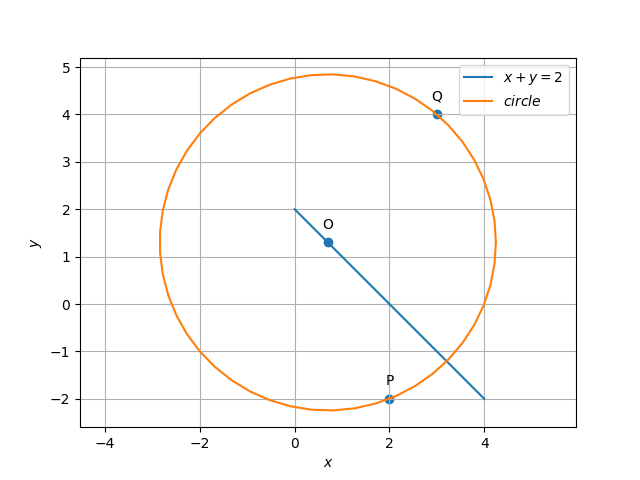
\includegraphics[width=\columnwidth]{./figs/circex/CircOr.eps}
\caption{Circle passing through $\myvec{2\\-2},\myvec{3\\4}$. Center is on line $\myvec{1 & 1}\vec{x}=2$. }
\label{fig:CircOr}	
\end{figure}

\item 
Find the points on the curve  
%\cite{twelve_one}
\begin{align}
x^2+y^2-2x-3 = 0
\label{eq:circle_tangent_prob}
\end{align}
at which the tangents are parallel to the $x$-axis.
\\
\solution \eqref{eq:circle_tangent_prob} can be expressed as
\begin{align}
\vec{x}^T\vec{x}+\myvec{-2 & 0}\vec{x}-3 &= 0
\label{eq:circle_tangent_prob_vec}
\\
\implies \vec{V} = \vec{I}, \vec{u} = \myvec{-1 \\ 0}, f = -3
\label{eq:circle_tangent_prob_uf}
\end{align}
From Table \ref{table:conics}, the centre and radius are
\begin{align}
\vec{c} = -\vec{u} = \myvec{-1 \\ 0}, r =\sqrt{\norm{\vec{u}}^2-f} = 2
\end{align}
$\because$ the tangents are parallel to the $x$-axis, their direction and normal vectors are respectively,
\begin{align}
\vec{m} = \myvec{1\\0},
\vec{n} = \myvec{0\\1}.
\end{align}
From Table \ref{table:conics},
\begin{align}
\kappa = \pm \sqrt{\frac{\vec{u}^T\vec{u}-f}{\vec{n}^T\vec{n}}} = \pm \sqrt{\frac{4}{1}} = \pm 2
\end{align}
and the desired points of contact are 
\begin{align}
\vec{q}_1, \vec{q}_2 = \myvec{1\\0}\pm 2\myvec{0\\1} =  
\myvec{1 \\  2},
\myvec{1 \\  -2}
\end{align}
%
Fig. \ref{fig:CircOr}	verifies the above results.
\begin{figure}[!ht]
\centering
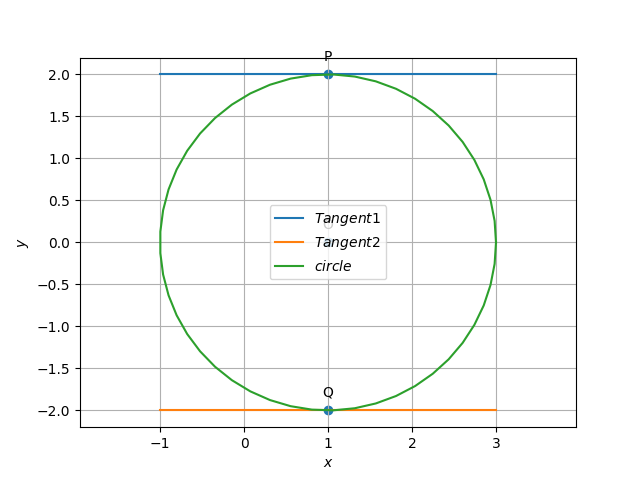
\includegraphics[width=\columnwidth]{./figs/circex/CircTangent.eps}
\caption{Tangents are parallel to the $x$-axis. }
\label{fig:CircTangent}	
\end{figure}

\end{enumerate}
}
\caption{}
\label{fig:8.5.16_circle_latex}	
\end{figure}
%
%
%\renewcommand{\thefigure}{\theenumi}
%
\item {\em Construction: }In Fig. \ref{fig:8.5.16_circle_latex} the known parameters are
%\label{}
\\
%
%\solution From the given information, 
%$\triangle ABC$ are 
\begin{align}
\vec{O} &= \myvec{0\\0} ,
\\
\vec{A} &= \myvec{r\\0} ,
\label{eq:8.5.16_constr_a}
\\
 \vec{B} &= \myvec{-r\\0} 
\label{eq:8.5.16_constr_b}
\\
\vec{C}&= r\myvec{\cos\theta\\\sin\theta}
\label{eq:8.5.16_constr_cgen}
\end{align}
%
Let 
\begin{align}
\vec{D} & = r\myvec{\cos\theta_1\\\sin\theta_1} 
\label{eq:8.5.16_constr_dgen}
\end{align}
From the given information,
\begin{align}
 \norm{\vec{D} - \vec{C}} &= r
\\
\implies \brak{\vec{D} - \vec{C}}^T\brak{\vec{D} - \vec{C}} &= r^2\\
 \label{eq:8.5.16_dist_formula}
\\
\implies  \norm{D} ^2 - 2\vec{D}^T\vec{C} +  \norm{C}^2 &=r^2 
\end{align}
In the above, 
\begin{align}
\because \norm{D} &= \norm{\vec{C}} = r,
\\
\frac{\vec{D}^T\vec{C}}{\norm{D}\norm{C}}  &= \frac{1}{2}
\\
\implies \cos \brak{\theta_1-\theta} &= 60 \degree
\label{eq:8.5.16_theta_diff}
\end{align}
using the definition of the inner product.  $\because \theta$ is known, we get $\theta_1$ from \eqref{eq:8.5.16_theta_diff}
and $\vec{D}$ from 
\eqref{eq:8.5.16_constr_dgen}. 
%
\subitem Thus,
\begin{align}
BD: \vec{x} &= \vec{B} + \lambda_1 \brak{\vec{B}-\vec{D}}
\\
AC: \vec{x} &= \vec{A} + \lambda_2 \brak{\vec{A}-\vec{C}}
\end{align}
%
which can be used to obtain $\vec{E}$.


%
General equation of conics is 
\begin{align}
    \vec{x}^T\vec{V}\vec{x}+ 2\vec{u}^T\vec{x}+f = 0
    \label{eq:solutions/1/16/eq:1}
\end{align}
Comparing with the equation given,
\begin{align}
\vec{V}=\myvec{\frac{1}{9} & 0 \\ 0 & \frac{1}{16}}\\
\vec{u}=\vec{0}\\
f=-1\\
\mydet{\vec{v}}=\mydet{\myvec{\frac{1}{9} & 0 \\ 0 & \frac{1}{16}}}>0
\end{align}
$\because \abs{\vec{V}}>0$, the given equation is of ellipse.\\
a)The tangents are parallel to the x-axis, hence, their direction and normal vectors, $\vec{m_1}$ and $\vec{n_1}$ are respectively,
\begin{align}
\vec{m_1}=\myvec{1\\0}\\
\vec{n_1}=\myvec{0\\1}
\end{align}
For an ellipse, given the normal vector $\vec{n}$, the tangent points of contact to the ellipse are given by
\begin{align}
    \vec{q}=\vec{V}^{-1}(\kappa \vec{n}-\vec{u})
    \label{eq:solutions/1/16/eq:2}
    =\vec{V}^{-1}\kappa \vec{n}
\end{align}
where
\begin{align}
    \kappa=\pm \sqrt{\frac{\vec{u^T}\vec{V}^{-1}\vec{u}-f}{\vec{n^T}\vec{V}^{-1}\vec{n}}}
    \label{eq:solutions/1/16/eq:2.0.9}\\
   =\pm \sqrt{\frac{-f}{\vec{n^T}\vec{V}^{-1}\vec{n}}}\\
    \vec{V}^{-1}=\myvec{9 & 0 \\ 0 & 16}\\
    \kappa_1=\pm \sqrt{\frac{-(-1)}{\myvec{0 & 1}\myvec{9 & 0 \\ 0 & 16} \myvec{0\\1}}}\\
 \implies \kappa_1=\pm \sqrt{\frac{1}{16}}\\
    \implies \kappa_1=\pm \frac{1}{4}      
\end{align}
From \eqref{eq:solutions/1/16/eq:2} , the point of contact $\vec{q_i}$ are,
\begin{align}
    \vec{q_1}=\myvec{9 & 0 \\ 0 & 16}\frac{1}{4}\myvec{0\\1}\\
    =\myvec{9 & 0 \\ 0 & 16}\myvec{0\\\frac{1}{4}}\\
    =\myvec{0\\4}\\
    \vec{q_2}=\myvec{9 & 0 \\ 0 & 16}\left(-\frac{1}{4}\right)\ \myvec{0\\1}\\
    =\myvec{9 & 0 \\ 0 & 16}\myvec{0\\-\frac{1}{4}}\\
    =\myvec{0\\-4}
\end{align}
b) The tangents are parallel to the y-axis, hence, their direction and normal vectors, $\vec{m_2}$ and $\vec{n_2}$ are respectively,
\begin{align}
\vec{m_2}=\myvec{0\\1}\\
\vec{n_2}=\myvec{1\\0}
\end{align}
Using equation \eqref{eq:solutions/1/16/eq:2.0.9}, the values of $\kappa$ for this case are
\begin{align}
     \kappa_2=\pm \sqrt{\frac{-(-1)}{\myvec{1 & 0}\myvec{9 & 0 \\ 0 & 16} \myvec{1\\0}}}\\
 \implies \kappa_2=\pm \sqrt{\frac{1}{9}}\\
    \implies \kappa_2=\pm \frac{1}{3} 
\end{align}
and from \eqref{eq:solutions/1/16/eq:2} , the point of contact $\vec{q_i}$ are,
\begin{align}
\vec{q_3}=\myvec{9 & 0 \\ 0 & 16}\frac{1}{3}\myvec{1\\0}\\
    =\myvec{9 & 0 \\ 0 & 16}\myvec{\frac{1}{3}\\0}\\
    =\myvec{3\\0}\\
\vec{q_4}=\myvec{9 & 0 \\ 0 & 16}\left(-\frac{1}{3}\right)\ \myvec{1\\0}\\
    =\myvec{9 & 0 \\ 0 & 16}\myvec{-\frac{1}{3}\\0}\\
    =\myvec{-3\\0}
\end{align}
 \begin{figure}[h!]
	\centering
	\includegraphics[width=\columnwidth]{./solutions/conics/1/16/ellipse.png}
	\caption{Figure depicting point of contact of tangents of ellipse parallel to x-axis and y-axis}
	\label{eq:solutions/1/16/fig1}
\end{figure}

%\end{enumerate}

\item $O$ is a point in the interior of $\triangle PQR$.  $A, B and C$ are points on $OP, OQ$ and $OR$ respectively such that $AB  \parallel  PQ$ and $AC  \parallel  PR$. Show that $BC  \parallel  QR$.
%
\item $ABCD$ is a trapezium in which $AB  \parallel  DC$ and its diagonals intersect each other at the point $O$. Show
that
$\frac{AO}{ BO}=\frac{CO}{  DO}$
%
\item The diagonals of a quadrilateral $ABCD$ intersect each other at the point $O$ such that $\frac{AO}{ BO}=\frac{CO}{  DO}$.   Show that $ABCD$ is a trapezium.
%
\item $PQ \parallel RS$ and $PS$ intersects $QR$ at $O$.  Show that $\triangle OPQ \sim \triangle ORS$.
 \item $CM$ and $RN$ are respectively the medians of $ \triangle  ABC$ and $ \triangle  PQR$. If $ \triangle  ABC  \sim   \triangle  PQR$, prove that 
\begin{enumerate}
\item  $ \triangle  AMC  \sim   \triangle  PNR$ 
\item  $\frac{CM}{RN}=\frac{ AB}{  PQ}$
\item $ \triangle  CMB  \sim   \triangle  RNQ$
%
\end{enumerate}
\item Diagonals $AC$ and $BD$ of a trapezium $ABCD$ with $AB  \parallel  DC$ intersect each other at the point $O$. Using a similarity criterion for two triangles, show that
$\frac{OA}{OC} =  \frac{OB}  {OD}$
%
\item In $\triangle PQR$, $QP$ is extended to $T$ and $S$ is a point on $QR$ such that $ \frac{QR}{QS}=\frac{ QT}{  PR}$. If $\angle PRQ = \angle PQS$, show that 
 that  $\triangle  PQS  \sim   \triangle  TQR$.
\item $S$ and $T$ are points on sides $PR$ and $QR$ of $\triangle PQR$ such that $\angle P = \angle 
 RTS$. Show that $\triangle RPQ \sim \triangle RTS$.
\item  In $\triangle ABC$, $D$ and $E$ are points on the sides $AB$ and $AC$ respectively.  If  $\triangle  ABE \cong   \triangle  ACD$, show that  $\triangle  ADE  \sim   \triangle  ABC$.
\item   Altitudes $AD$ and CE of  $\triangle  ABC$ intersect each other at the point $P$. Show that:
%
\begin{enumerate}
\item   $\triangle  AEP  \sim   \triangle  CDP $
\item   $\triangle  ABD  \sim   \triangle  CBE $
\item   $\triangle  AEP  \sim   \triangle  ADB$
 \item  $\triangle  PDC  \sim   \triangle  BEC$
\end{enumerate}
%
\item  $E$ is a point on the side $AD$ produced of a parallelogram $ABCD$ and $BE$ intersects $CD$ at $F$. Show that  $\triangle  ABE  \sim   \triangle  CFB$.
\item  $ABC$ and $AMP$ are two right triangles, right angled at $B$ and $M$ respectively. $M$ lies on $AC$ and $AB$ is extended to meet $P$. Prove that: 
\begin{enumerate}
\item   $\triangle  ABC  \sim   \triangle  AMP$
\item  $\frac{CA}{PA} = \frac{BC}{  MP}$
\end{enumerate}
%
\item  $CD$ and $GH$ are respectively the bisectors of  $\angle  ACB$ and  $\angle  EGF$ such that $D$ and $H$ lie on sides $AB$ and $FE$ of  $\triangle  ABC$ and  $\triangle  EFG$ respectively. If  $\triangle  ABC  \sim   \triangle  FEG$, show that:
\item  $\frac{CD}{GH} = \frac{ AC}{  FG}$
\item  $ \triangle  DCB  \sim   \triangle  HGE$
 \item  $ \triangle  DCA  \sim   \triangle  HGF$
\item  $E$ is a point on side $CB$ produced of an isosceles $\triangle ABC$ with $AB = AC$. If $AD  \perp  BC$ and $EF  \perp  AC$, prove that  $\triangle  ABD  \sim   \triangle  ECF$.
\item  Sides $AB$ and $BC$ and median $AD$ of a $\triangle ABC$ are respectively proportional to sides  $PQ$  and $QR$ and median $PM$ of  $\triangle PQR$. Show that  $\triangle  ABC  \sim  \triangle PQR$ .
\item  $D$ is a point on the side $BC$ of a $\triangle ABC$ such that  $\angle  ADC =  \angle  BAC$. Show that $CA^2 = CB.CD$.
\item  Sides $AB$ and $AC$ and median $AD$ of a $\triangle ABC$ are respectively proportional to sides $PQ$ and $PR$ and median $PM$ of another $\triangle PQR$. Show that  $\triangle  ABC  \sim   \triangle PQR$ .%
\item  If $AD$ and $PM$ are medians of $\triangle s ABC$ and $PQR$, respectively where  $\triangle  ABC  \sim   \triangle PQR$ , prove that
$\frac{AB}{ PQ} = \frac{AD}{  PM}$
\item The line segment $XY$ is parallel to side $AC$ of  $\triangle  ABC$ and it divides the triangle into two parts of equal areas. Find the ratio
$\frac{AX}{ AB}$
% 
\item  Diagonals of a trapezium $ABCD$ with $AB  \parallel  DC$ intersect each other at the point $O$. If $AB = 2 CD$, find the ratio of the areas of $\triangle s AOB$ and $COD$.
\item  $ABC$ and $DBC$ are two triangles on the same base $BC$. If $AD$ intersects $BC$ at $O$, show that
$\frac{ar (ABC)}{ ar (DBC)}=\frac{AO}{  DO}$.
\item  If the areas of two similar triangles are equal, prove that they are congruent.
\item  $D, E$ and $F$ are respectively the mid-points of sides $AB$, $BC$ and $CA$ of  $\triangle  ABC$. Find the ratio of the areas of  $\triangle  DEF$ and  $\triangle  ABC$.
\item  Prove that the ratio of the areas of two similar triangles is equal to the square of the ratio of their corresponding medians.
\item  Prove that the area of an equilateral triangle described on one side of a square is equal to half the area of the equilateral triangle described on one of its diagonals.
\item $ABC$ and $BDE$ are two equilateral triangles such that $D$ is the mid-point of $BC$. Find the ratio of the areas of triangles $ABC$ and $BDE$.
\item The sides of two similar triangles are in the ratio 4 : 9. Find the ratio the area of  these triangles are in the ratio
\item In $\triangle ABC, \angle  ACB = 90\degree$ and $CD  \perp  AB$. Prove that 
$\frac{BC^2}{AC^2} = \frac{BD}{ AD}$.
\item In $\triangle ABC$,  if $AD  \perp  BC$, prove that $AB^2+ CD^2 = BD^2 + AC^2$.
\item $BL$ and $CM$ are medians of a $\triangle ABC$ right angled at $A$. Prove that $4 (BL^2 + CM^2
) = 5 BC^2$ .
\item $O$ is any point inside a rectangle $ABCD$. Prove that $OB^2+OD^2 = OA^2+OC^2$.
\item  $PQR$ is a triangle right angled at $P$ and $M$ is a point on $QR$ such that $PM  \perp  QR$. Show that $PM^2= QM . MR$.
\item  $ABD$ is a triangle right angled at $A$ and $AC \perp  BD$. Show that
\begin{enumerate}
\item  $AB^2 = BC . BD$
\item  $AC^2 = BC . DC$
\item  $AD^2  = BD . CD$
\end{enumerate}
\item  $ABC$ is an isosceles triangle right angled at $C$. Prove that $AB^2= 2 AC^2$.
 \item  $ABC$ is an isosceles triangle with $AC = BC$. If $AB^2=2 AC^2$, prove that $ABC$ is a right triangle.
\item  $ABC$ is an equilateral triangle of side $2a$. Find each of its altitudes. 
\item  Prove that the sum of the squares of the sides of a rhombus is equal to the sum of the squares of its diagonals.
\item  $O$ is a point in the interior of a $\triangle ABC, OD  \perp  BC, OE  \perp  AC and OF  \perp  AB$. Show that
%
\begin{enumerate}
\item  $OA^2 + OB^2 + BD^2 – OD2 – OE2– OF2 = AF^2 + BD^2 + CE^2$.
\item  $AF^2 + BD^2 +CE^2 = AE^2 + CD^2 + BF^2$.
\end{enumerate}
\item  $D$ and $E$ are points on the sides $CA$ and $CB$ respectively of a $\triangle ABC$ right angled at $C$. Prove that $AE^2+ BD^2 = AB^2 + DE^2$.
\item  The perpendicular from $A$ on side $BC$ of a  $\triangle  ABC$ intersects $BC$ at $D$ such that $DB = 3 CD$. Prove that $2 AB^2= 2 AC^2 + BC^2$ .
\item  In an equilateral $\triangle ABC$, $D$ is a point on side $BC$ such that $BD = \frac{1}{3} BC$.  Prove that $9 AD^2= 7 AB^2$.
\item  In an equilateral triangle, prove that three times the square of one side is equal to four times the square of one of its altitudes.
\item  $PS$ is the bisector of  $\angle  QPR$ of  $\triangle PQR$ . Prove that
$\frac{QS}{SR} = \frac{PQ}{PR}$
\item $D$ is a point on hypotenuse $AC$ of  $\triangle  ABC$, such that $BD  \perp  AC, DM  \perp  BC$ and $DN  \perp  AB$. Prove that :
\begin{enumerate}
\item  DM2 = DN . MC  
 \item  DN2 = DM . AN
\end{enumerate}

\item  $ABC$ is a triangle in which  $\angle  ABC > 90\degree$ and $AD  \perp  CB$ produced. Prove that
$ AC^2= AB^2 + BC^2 + 2 BC . BD$.
\item $ABC$ is a triangle in which  $\angle  ABC < 90\degree$ and $AD  \perp  BC$. Prove that $AC^2= AB^2 + BC^2 – 2 BC . BD$.
\item $AD$ is a median of a $\triangle ABC$ and $AM  \perp  BC$. Prove that :
\begin{enumerate}
\item  $AC^2 = AD^2 + BC . DM +
\brak{\frac{BC}{ 2}}^2$
\\
\solution

General equation of conics is 
\begin{align}
    \vec{x}^T\vec{V}\vec{x}+ 2\vec{u}^T\vec{x}+f = 0
    \label{eq:solutions/1/16/eq:1}
\end{align}
Comparing with the equation given,
\begin{align}
\vec{V}=\myvec{\frac{1}{9} & 0 \\ 0 & \frac{1}{16}}\\
\vec{u}=\vec{0}\\
f=-1\\
\mydet{\vec{v}}=\mydet{\myvec{\frac{1}{9} & 0 \\ 0 & \frac{1}{16}}}>0
\end{align}
$\because \abs{\vec{V}}>0$, the given equation is of ellipse.\\
a)The tangents are parallel to the x-axis, hence, their direction and normal vectors, $\vec{m_1}$ and $\vec{n_1}$ are respectively,
\begin{align}
\vec{m_1}=\myvec{1\\0}\\
\vec{n_1}=\myvec{0\\1}
\end{align}
For an ellipse, given the normal vector $\vec{n}$, the tangent points of contact to the ellipse are given by
\begin{align}
    \vec{q}=\vec{V}^{-1}(\kappa \vec{n}-\vec{u})
    \label{eq:solutions/1/16/eq:2}
    =\vec{V}^{-1}\kappa \vec{n}
\end{align}
where
\begin{align}
    \kappa=\pm \sqrt{\frac{\vec{u^T}\vec{V}^{-1}\vec{u}-f}{\vec{n^T}\vec{V}^{-1}\vec{n}}}
    \label{eq:solutions/1/16/eq:2.0.9}\\
   =\pm \sqrt{\frac{-f}{\vec{n^T}\vec{V}^{-1}\vec{n}}}\\
    \vec{V}^{-1}=\myvec{9 & 0 \\ 0 & 16}\\
    \kappa_1=\pm \sqrt{\frac{-(-1)}{\myvec{0 & 1}\myvec{9 & 0 \\ 0 & 16} \myvec{0\\1}}}\\
 \implies \kappa_1=\pm \sqrt{\frac{1}{16}}\\
    \implies \kappa_1=\pm \frac{1}{4}      
\end{align}
From \eqref{eq:solutions/1/16/eq:2} , the point of contact $\vec{q_i}$ are,
\begin{align}
    \vec{q_1}=\myvec{9 & 0 \\ 0 & 16}\frac{1}{4}\myvec{0\\1}\\
    =\myvec{9 & 0 \\ 0 & 16}\myvec{0\\\frac{1}{4}}\\
    =\myvec{0\\4}\\
    \vec{q_2}=\myvec{9 & 0 \\ 0 & 16}\left(-\frac{1}{4}\right)\ \myvec{0\\1}\\
    =\myvec{9 & 0 \\ 0 & 16}\myvec{0\\-\frac{1}{4}}\\
    =\myvec{0\\-4}
\end{align}
b) The tangents are parallel to the y-axis, hence, their direction and normal vectors, $\vec{m_2}$ and $\vec{n_2}$ are respectively,
\begin{align}
\vec{m_2}=\myvec{0\\1}\\
\vec{n_2}=\myvec{1\\0}
\end{align}
Using equation \eqref{eq:solutions/1/16/eq:2.0.9}, the values of $\kappa$ for this case are
\begin{align}
     \kappa_2=\pm \sqrt{\frac{-(-1)}{\myvec{1 & 0}\myvec{9 & 0 \\ 0 & 16} \myvec{1\\0}}}\\
 \implies \kappa_2=\pm \sqrt{\frac{1}{9}}\\
    \implies \kappa_2=\pm \frac{1}{3} 
\end{align}
and from \eqref{eq:solutions/1/16/eq:2} , the point of contact $\vec{q_i}$ are,
\begin{align}
\vec{q_3}=\myvec{9 & 0 \\ 0 & 16}\frac{1}{3}\myvec{1\\0}\\
    =\myvec{9 & 0 \\ 0 & 16}\myvec{\frac{1}{3}\\0}\\
    =\myvec{3\\0}\\
\vec{q_4}=\myvec{9 & 0 \\ 0 & 16}\left(-\frac{1}{3}\right)\ \myvec{1\\0}\\
    =\myvec{9 & 0 \\ 0 & 16}\myvec{-\frac{1}{3}\\0}\\
    =\myvec{-3\\0}
\end{align}
 \begin{figure}[h!]
	\centering
	\includegraphics[width=\columnwidth]{./solutions/conics/1/16/ellipse.png}
	\caption{Figure depicting point of contact of tangents of ellipse parallel to x-axis and y-axis}
	\label{eq:solutions/1/16/fig1}
\end{figure}

\item  $AB^2 = AD^2 – BC . DM + \brak{\frac{BC}{ 2}}^
2 $
\\
\solution
%
General equation of conics is 
\begin{align}
    \vec{x}^T\vec{V}\vec{x}+ 2\vec{u}^T\vec{x}+f = 0
    \label{eq:solutions/1/16/eq:1}
\end{align}
Comparing with the equation given,
\begin{align}
\vec{V}=\myvec{\frac{1}{9} & 0 \\ 0 & \frac{1}{16}}\\
\vec{u}=\vec{0}\\
f=-1\\
\mydet{\vec{v}}=\mydet{\myvec{\frac{1}{9} & 0 \\ 0 & \frac{1}{16}}}>0
\end{align}
$\because \abs{\vec{V}}>0$, the given equation is of ellipse.\\
a)The tangents are parallel to the x-axis, hence, their direction and normal vectors, $\vec{m_1}$ and $\vec{n_1}$ are respectively,
\begin{align}
\vec{m_1}=\myvec{1\\0}\\
\vec{n_1}=\myvec{0\\1}
\end{align}
For an ellipse, given the normal vector $\vec{n}$, the tangent points of contact to the ellipse are given by
\begin{align}
    \vec{q}=\vec{V}^{-1}(\kappa \vec{n}-\vec{u})
    \label{eq:solutions/1/16/eq:2}
    =\vec{V}^{-1}\kappa \vec{n}
\end{align}
where
\begin{align}
    \kappa=\pm \sqrt{\frac{\vec{u^T}\vec{V}^{-1}\vec{u}-f}{\vec{n^T}\vec{V}^{-1}\vec{n}}}
    \label{eq:solutions/1/16/eq:2.0.9}\\
   =\pm \sqrt{\frac{-f}{\vec{n^T}\vec{V}^{-1}\vec{n}}}\\
    \vec{V}^{-1}=\myvec{9 & 0 \\ 0 & 16}\\
    \kappa_1=\pm \sqrt{\frac{-(-1)}{\myvec{0 & 1}\myvec{9 & 0 \\ 0 & 16} \myvec{0\\1}}}\\
 \implies \kappa_1=\pm \sqrt{\frac{1}{16}}\\
    \implies \kappa_1=\pm \frac{1}{4}      
\end{align}
From \eqref{eq:solutions/1/16/eq:2} , the point of contact $\vec{q_i}$ are,
\begin{align}
    \vec{q_1}=\myvec{9 & 0 \\ 0 & 16}\frac{1}{4}\myvec{0\\1}\\
    =\myvec{9 & 0 \\ 0 & 16}\myvec{0\\\frac{1}{4}}\\
    =\myvec{0\\4}\\
    \vec{q_2}=\myvec{9 & 0 \\ 0 & 16}\left(-\frac{1}{4}\right)\ \myvec{0\\1}\\
    =\myvec{9 & 0 \\ 0 & 16}\myvec{0\\-\frac{1}{4}}\\
    =\myvec{0\\-4}
\end{align}
b) The tangents are parallel to the y-axis, hence, their direction and normal vectors, $\vec{m_2}$ and $\vec{n_2}$ are respectively,
\begin{align}
\vec{m_2}=\myvec{0\\1}\\
\vec{n_2}=\myvec{1\\0}
\end{align}
Using equation \eqref{eq:solutions/1/16/eq:2.0.9}, the values of $\kappa$ for this case are
\begin{align}
     \kappa_2=\pm \sqrt{\frac{-(-1)}{\myvec{1 & 0}\myvec{9 & 0 \\ 0 & 16} \myvec{1\\0}}}\\
 \implies \kappa_2=\pm \sqrt{\frac{1}{9}}\\
    \implies \kappa_2=\pm \frac{1}{3} 
\end{align}
and from \eqref{eq:solutions/1/16/eq:2} , the point of contact $\vec{q_i}$ are,
\begin{align}
\vec{q_3}=\myvec{9 & 0 \\ 0 & 16}\frac{1}{3}\myvec{1\\0}\\
    =\myvec{9 & 0 \\ 0 & 16}\myvec{\frac{1}{3}\\0}\\
    =\myvec{3\\0}\\
\vec{q_4}=\myvec{9 & 0 \\ 0 & 16}\left(-\frac{1}{3}\right)\ \myvec{1\\0}\\
    =\myvec{9 & 0 \\ 0 & 16}\myvec{-\frac{1}{3}\\0}\\
    =\myvec{-3\\0}
\end{align}
 \begin{figure}[h!]
	\centering
	\includegraphics[width=\columnwidth]{./solutions/conics/1/16/ellipse.png}
	\caption{Figure depicting point of contact of tangents of ellipse parallel to x-axis and y-axis}
	\label{eq:solutions/1/16/fig1}
\end{figure}

\item  $AC^2 + AB^2 = 2 AD^2 + \frac{1}{ 2} BC^2$
\end{enumerate}
\item Prove that the sum of the squares of the diagonals of parallelogram is equal to the sum of the squares of its sides.
\\
\solution

General equation of conics is 
\begin{align}
    \vec{x}^T\vec{V}\vec{x}+ 2\vec{u}^T\vec{x}+f = 0
    \label{eq:solutions/1/16/eq:1}
\end{align}
Comparing with the equation given,
\begin{align}
\vec{V}=\myvec{\frac{1}{9} & 0 \\ 0 & \frac{1}{16}}\\
\vec{u}=\vec{0}\\
f=-1\\
\mydet{\vec{v}}=\mydet{\myvec{\frac{1}{9} & 0 \\ 0 & \frac{1}{16}}}>0
\end{align}
$\because \abs{\vec{V}}>0$, the given equation is of ellipse.\\
a)The tangents are parallel to the x-axis, hence, their direction and normal vectors, $\vec{m_1}$ and $\vec{n_1}$ are respectively,
\begin{align}
\vec{m_1}=\myvec{1\\0}\\
\vec{n_1}=\myvec{0\\1}
\end{align}
For an ellipse, given the normal vector $\vec{n}$, the tangent points of contact to the ellipse are given by
\begin{align}
    \vec{q}=\vec{V}^{-1}(\kappa \vec{n}-\vec{u})
    \label{eq:solutions/1/16/eq:2}
    =\vec{V}^{-1}\kappa \vec{n}
\end{align}
where
\begin{align}
    \kappa=\pm \sqrt{\frac{\vec{u^T}\vec{V}^{-1}\vec{u}-f}{\vec{n^T}\vec{V}^{-1}\vec{n}}}
    \label{eq:solutions/1/16/eq:2.0.9}\\
   =\pm \sqrt{\frac{-f}{\vec{n^T}\vec{V}^{-1}\vec{n}}}\\
    \vec{V}^{-1}=\myvec{9 & 0 \\ 0 & 16}\\
    \kappa_1=\pm \sqrt{\frac{-(-1)}{\myvec{0 & 1}\myvec{9 & 0 \\ 0 & 16} \myvec{0\\1}}}\\
 \implies \kappa_1=\pm \sqrt{\frac{1}{16}}\\
    \implies \kappa_1=\pm \frac{1}{4}      
\end{align}
From \eqref{eq:solutions/1/16/eq:2} , the point of contact $\vec{q_i}$ are,
\begin{align}
    \vec{q_1}=\myvec{9 & 0 \\ 0 & 16}\frac{1}{4}\myvec{0\\1}\\
    =\myvec{9 & 0 \\ 0 & 16}\myvec{0\\\frac{1}{4}}\\
    =\myvec{0\\4}\\
    \vec{q_2}=\myvec{9 & 0 \\ 0 & 16}\left(-\frac{1}{4}\right)\ \myvec{0\\1}\\
    =\myvec{9 & 0 \\ 0 & 16}\myvec{0\\-\frac{1}{4}}\\
    =\myvec{0\\-4}
\end{align}
b) The tangents are parallel to the y-axis, hence, their direction and normal vectors, $\vec{m_2}$ and $\vec{n_2}$ are respectively,
\begin{align}
\vec{m_2}=\myvec{0\\1}\\
\vec{n_2}=\myvec{1\\0}
\end{align}
Using equation \eqref{eq:solutions/1/16/eq:2.0.9}, the values of $\kappa$ for this case are
\begin{align}
     \kappa_2=\pm \sqrt{\frac{-(-1)}{\myvec{1 & 0}\myvec{9 & 0 \\ 0 & 16} \myvec{1\\0}}}\\
 \implies \kappa_2=\pm \sqrt{\frac{1}{9}}\\
    \implies \kappa_2=\pm \frac{1}{3} 
\end{align}
and from \eqref{eq:solutions/1/16/eq:2} , the point of contact $\vec{q_i}$ are,
\begin{align}
\vec{q_3}=\myvec{9 & 0 \\ 0 & 16}\frac{1}{3}\myvec{1\\0}\\
    =\myvec{9 & 0 \\ 0 & 16}\myvec{\frac{1}{3}\\0}\\
    =\myvec{3\\0}\\
\vec{q_4}=\myvec{9 & 0 \\ 0 & 16}\left(-\frac{1}{3}\right)\ \myvec{1\\0}\\
    =\myvec{9 & 0 \\ 0 & 16}\myvec{-\frac{1}{3}\\0}\\
    =\myvec{-3\\0}
\end{align}
 \begin{figure}[h!]
	\centering
	\includegraphics[width=\columnwidth]{./solutions/conics/1/16/ellipse.png}
	\caption{Figure depicting point of contact of tangents of ellipse parallel to x-axis and y-axis}
	\label{eq:solutions/1/16/fig1}
\end{figure}

\item   $D$ is a point on side $BC$ of  $\triangle  ABC$ such that
$\frac{BD}{CD} \frac{AB}{AC}  $.  Prove that $AD$ is the bisector of  $\angle  BAC$.
\end{enumerate}


